\documentclass[letterpaper,12pt]{article}

\usepackage{fullpage} % Package to use full page
\usepackage{parskip} % Package to tweak paragraph skipping
\usepackage{tikz} % Package for drawing
\usepackage{mathtools}
\usepackage[unicode]{hyperref}
\usepackage{amsfonts}
\usepackage{fancyhdr}
\usepackage{times}
\usepackage{changepage}
\usepackage{amssymb}
\usepackage{amsthm}
\usepackage{amsmath}
\usepackage[spanish,es-nodecimaldot]{babel}
\usepackage{graphicx}
\usepackage{subcaption}
\usepackage{float}
\usepackage[export]{adjustbox}
\usepackage{xcolor}
\usepackage{verbatim}

\hypersetup{
    colorlinks,
    linkcolor={blue!80!black},
    citecolor={blue!50!black},
    urlcolor={blue!80!black}
}
\theoremstyle{plain}
\newtheorem{theorem}{Theorem}

\usepackage{authblk} % Paquete para manejar autores y afiliaciones
\renewcommand\Authand{ y } % Cambiar "and" por "y"

\title{Trabajo práctico 2: Reconstrucción de Imágenes Tomográficas: Método Directo} % Título del documento

%\author[1]{Ignacio Lembo Ferrari \thanks{Correo electrónico: ignacio.lembo@ib.edu.ar}}
\author[1]{Ignacio Lembo Ferrari}
\affil[1]{Instituto Balseiro}
%\affil[2]{Departamento de Física, Universidad de Ejemplo}

\date{\vspace{-4ex}}

\begin{document}

\maketitle

\section{Reconstrucción de un fantoma Shepp-Logan}

\subsection{Generación del fantoma}

Utilizando el programa $\verb|CTSim|$ se generó un fantoma Shepp-Logan. Posteriormente, se rasterizó el fantoma obtenido (ver Fig. \ref{fig:SL_rast}) para observar los niveles de gris y se ecualizó el histograma de dicha imagen con $\verb|ImageJ|$ para ampliar su rango dinámico. El fantoma rasterizado y ecualizado se muestra en la Fig. \ref{fig:SL_EQ}.  

\begin{figure}[H]
   \centering
        \begin{subfigure}[h]{0.49\linewidth}
           \centering
           
\includegraphics[width=0.8\textwidth]{Figuras/SL_rasterizado.png}
           \caption{Fantoma rasterizado.} 
           \label{fig:SL_rast}
        \end{subfigure}
        \begin{subfigure}[h]{0.49\linewidth}
           \centering
           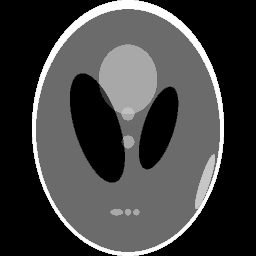
\includegraphics[width=0.8\textwidth]{Figuras/SL_rasterizado_EQ.png}
           \caption{Fantoma rasterizado y ecualizado.}
           \label{fig:SL_EQ}
        \end{subfigure}
   \caption{Fantoma de shepp-Logan rasterizado (a) y luego ecualizado (b).}
   \label{fig:SL}
\end{figure}

\subsection{Proyecciones del fantoma}

Se generaron proyecciones del fantoma Shepp-Logan utilizando los valores default del programa $\verb|CTSim|$. Estos valores son 367 detectores, 320 ángulos de proyección y 2 muestras por detector. De esta manera, se obtiene el sinograma que se muestra en la Fig. \ref{fig:SL_sinogram}, donde el eje horizontal representa los detectores y el eje vertical el ángulo de proyección.

\begin{figure}[H]
   \centering
         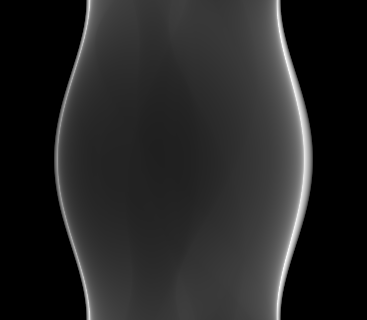
\includegraphics[width=0.5\textwidth]{Figuras/SL_sinogram.png}
   \caption{Sinograma del fantoma Shepp-Logan generado (Fig.\ref{fig:SL}).}
   \label{fig:SL_sinogram}
\end{figure}

\subsection{Error de reconstrucción del fanotoma}

El error de reconstrucción se calcula como la diferencia cuadratica media entre la imagen original y la imagen reconstruida de dimensiones $N\times M$, es decir
\begin{equation}
      \text{Error} = \sqrt{\frac{1}{NM}\sum_{x,y}(g(x,y) - f(x,y))^2}
\end{equation}
donde $g(x,y)$ es la imagen original y $f(x,y)$ es la imagen reconstruida. Se reconstruyó el fantoma Shepp-Logan utilizando retroproyección filtrada con filtro rampa a partir del sinograma de la Fig. \ref{fig:SL_sinogram}. El error de reconstrucción obtenido fue de $0.746177$. La imagen original, la reconstrucción y la diferencia entre ambas se muestran en la Fig. \ref{fig:sustraction}.

\begin{figure}[H]
   \centering
        \begin{subfigure}[h]{0.32\linewidth}
           \centering
           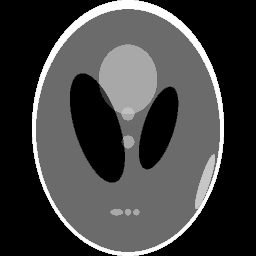
\includegraphics[width=\textwidth]{Figuras/SL_rasterizado_EQ.png}
           \caption{imagen original.} 
           \label{fig:original}
        \end{subfigure}
        \begin{subfigure}[h]{0.32\linewidth}
           \centering
           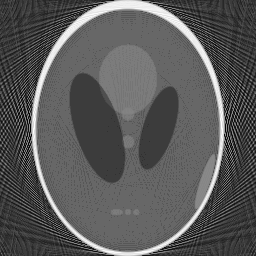
\includegraphics[width=\textwidth]{Figuras/SL_rec_lineal_EQ.png}
           \caption{Retroproyección filtrada.}
           \label{fig:reconstruccion}
        \end{subfigure}
        \begin{subfigure}[h]{0.32\linewidth}
         \centering
         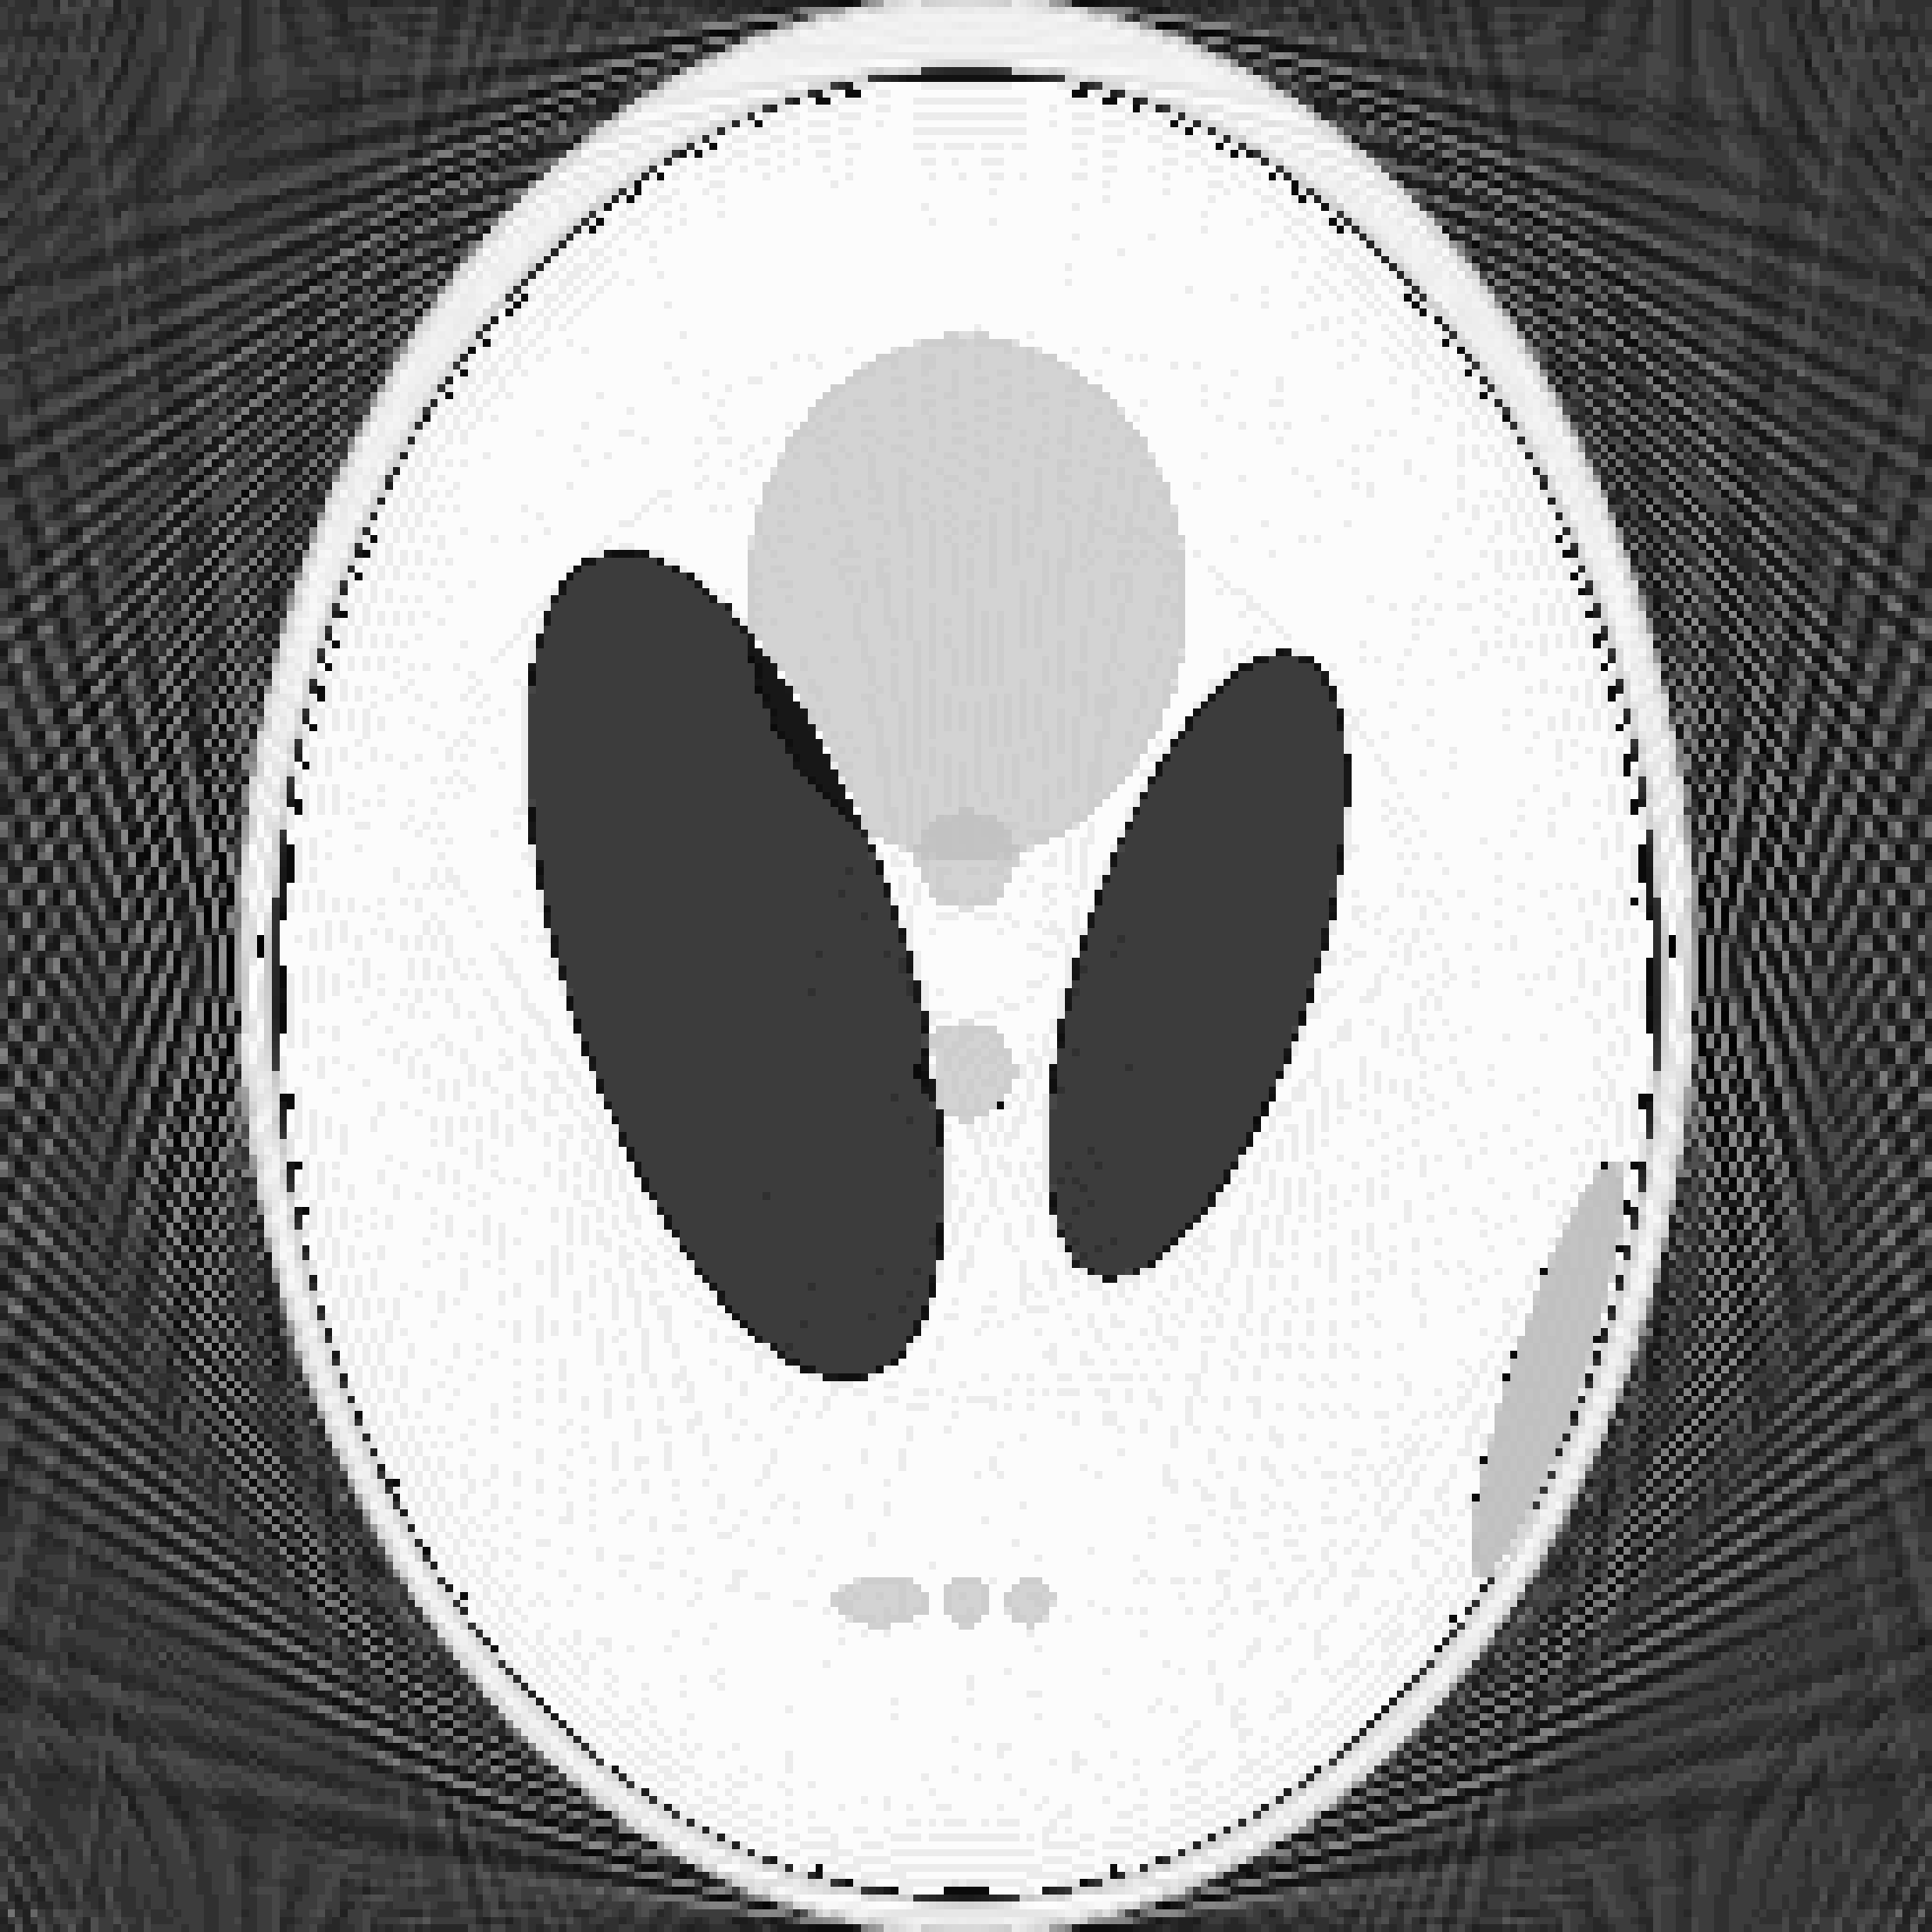
\includegraphics[width=\textwidth]{Figuras/sustraction.png}
         \caption{Diferencia entre (b) y (a).}
         \label{fig:resta}
      \end{subfigure}
   \caption{Fantoma de Shepp-Logan original (a), reconstrucción por retroproyección con filtro rampa a partir del sinograma de la Fig. \ref{fig:SL_sinogram} (b) y diferencia entre la imagen reconstruida y la original (c).}
   \label{fig:sustraction}
\end{figure}

\section{Error de reconstrucción en función de parámetros}

Se estudió el error de reconstrucción como función del número de detectores, y número de proyecciones (parámetros de adquisión) y del tipo de filtros (parámetro de reconstrucción). Para esto, se generaron fantomas de Shepp-Logan en $\verb|python|$ utilizando de base el programa \\$\verb|radon-skimage.py|$ provisto. En primer lugar, se varió el numero de detectores entre 25 y 1000 en intervalos de a 25 con 320 proyecciones y filtro rampa como se muestra en la Fig \ref{fig:err_det}. Se varío el número de proyecciones entre 20 y 800 en intervalos de 20 con 367 detectores y filtro rampa como se muestra en la Fig \ref{fig:err_proy}. Por último, se varió el tipo de filtro entre rampa, Hamming, Hanning y coseno con 367 detectores y 320 proyecciones como se muestra en la Fig \ref{fig:err_filtro}.

\begin{figure}[H]
   \centering
        \begin{subfigure}[h]{0.32\linewidth}
           \centering
           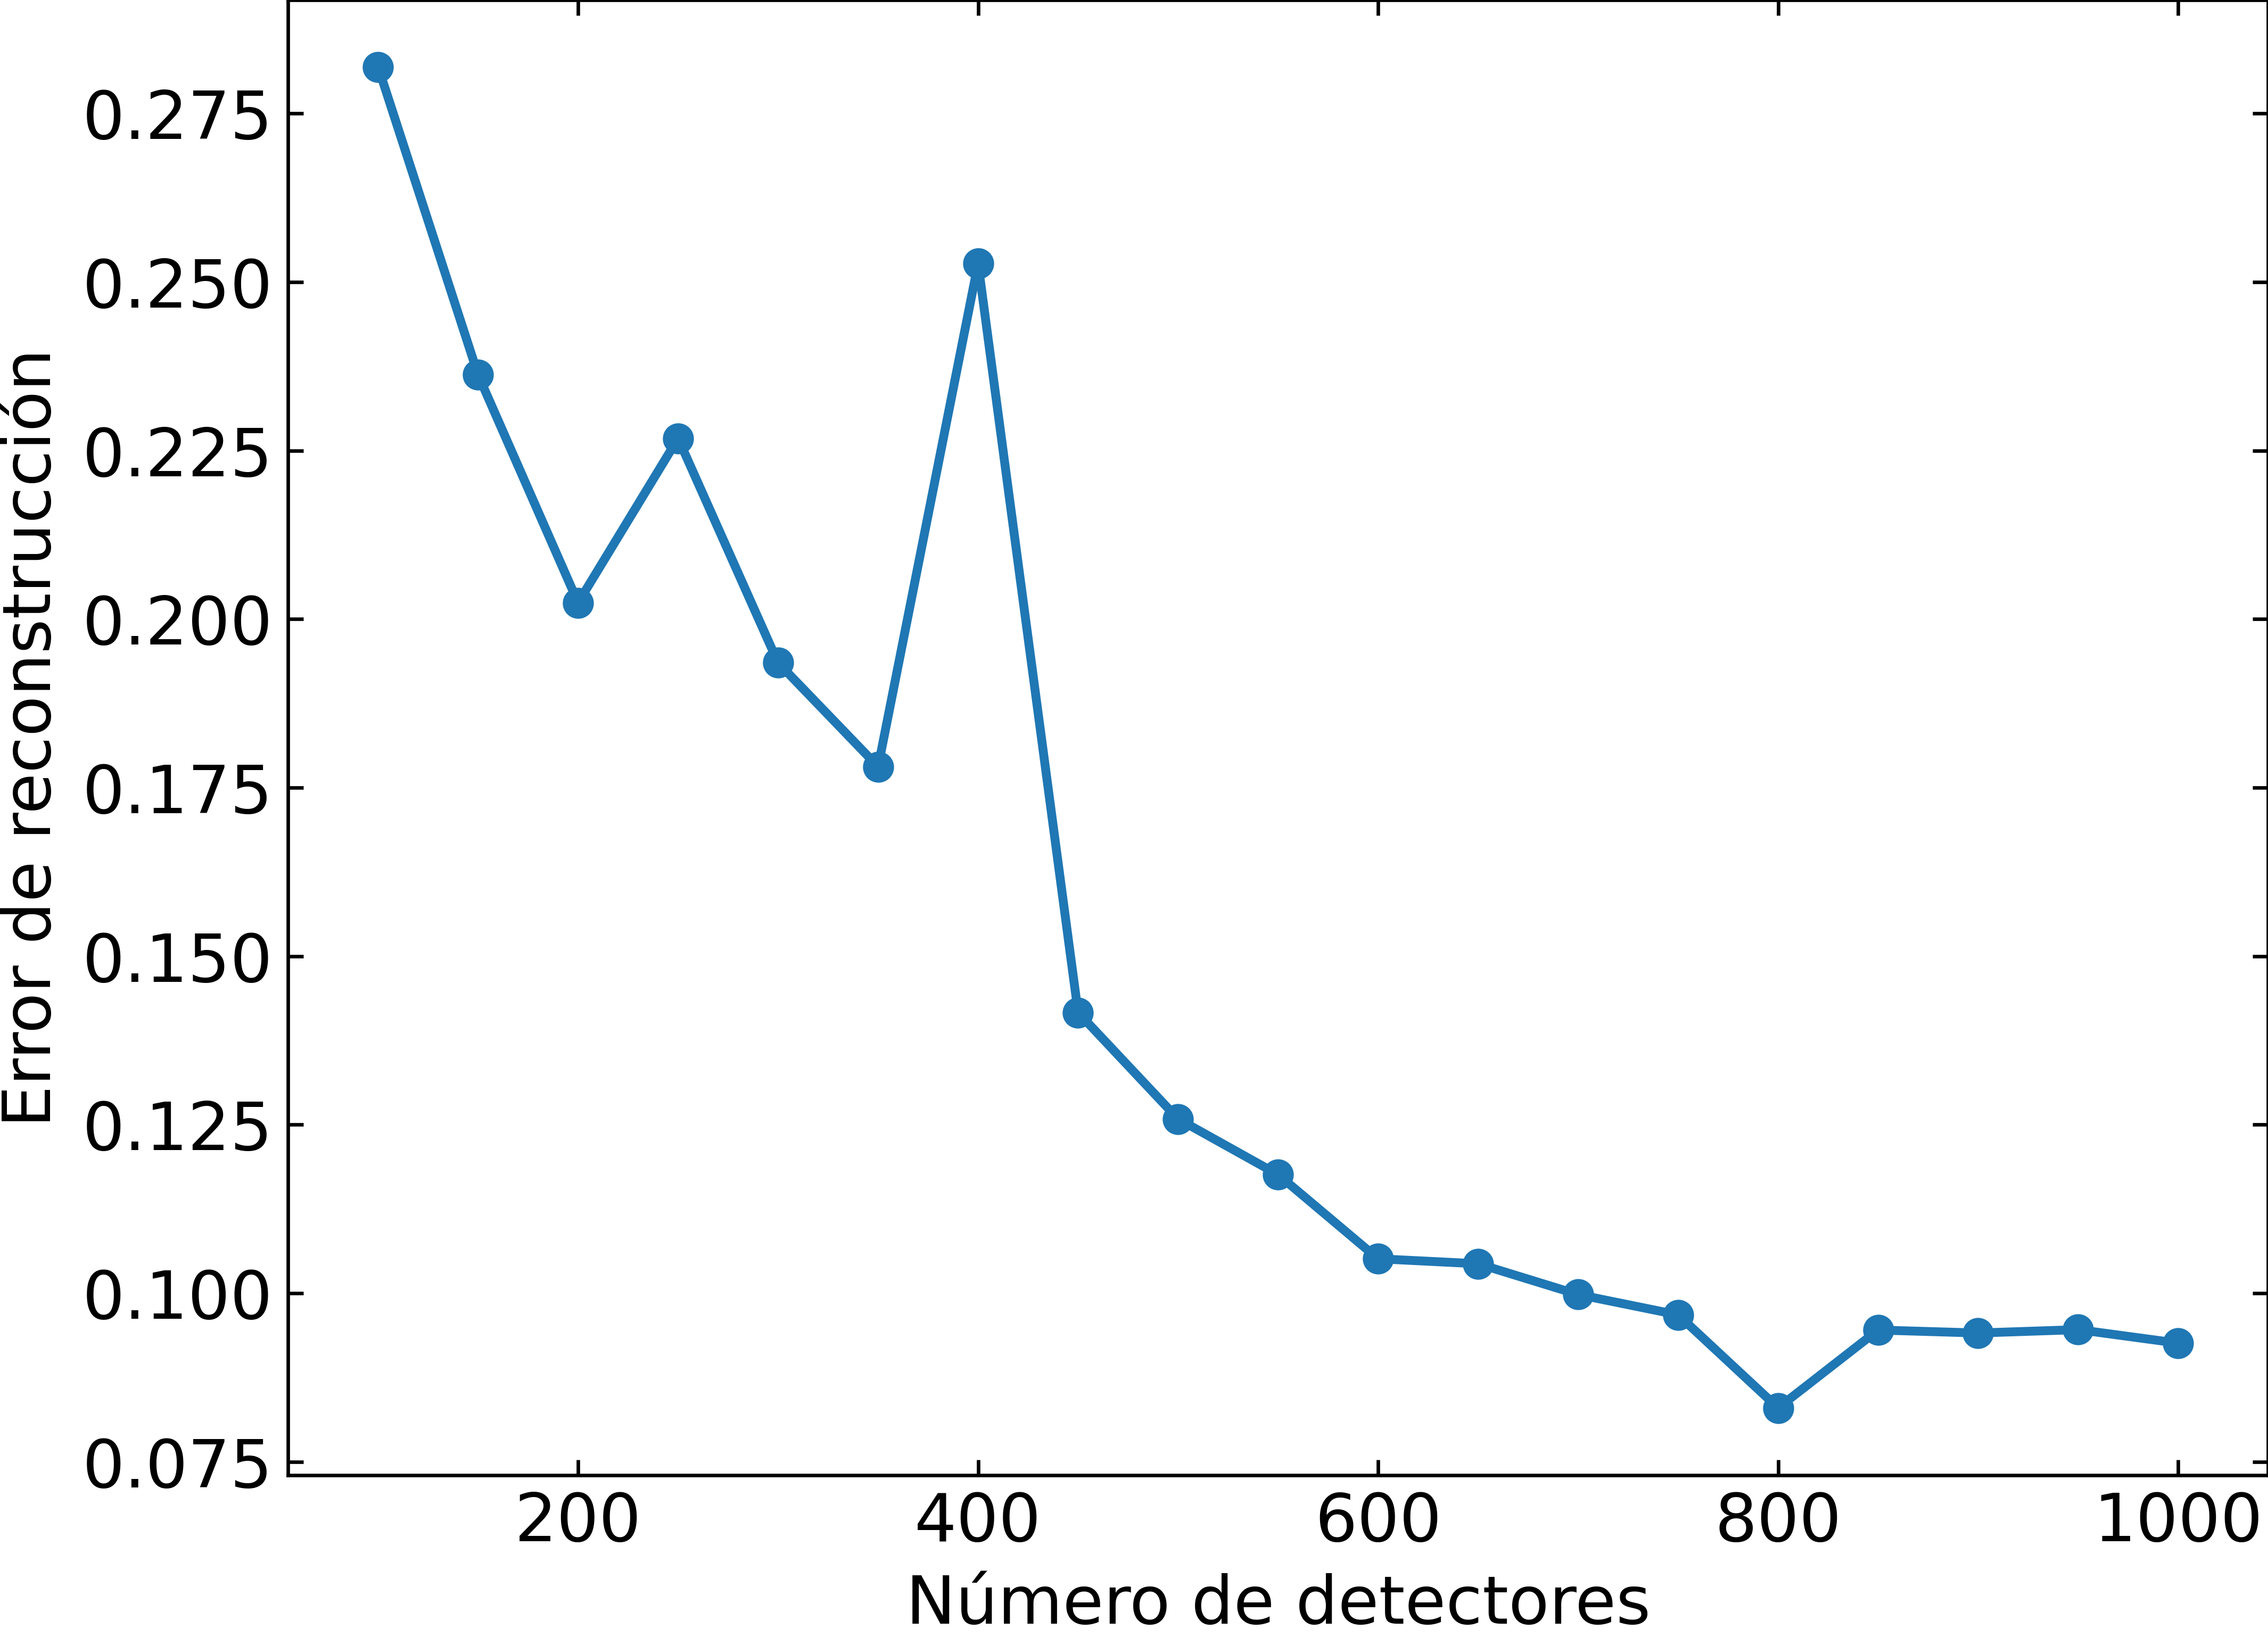
\includegraphics[width=\textwidth]{Figuras/error_vs_detectores.png}
           \caption{} 
           \label{fig:err_det}
        \end{subfigure}
        \begin{subfigure}[h]{0.32\linewidth}
           \centering
           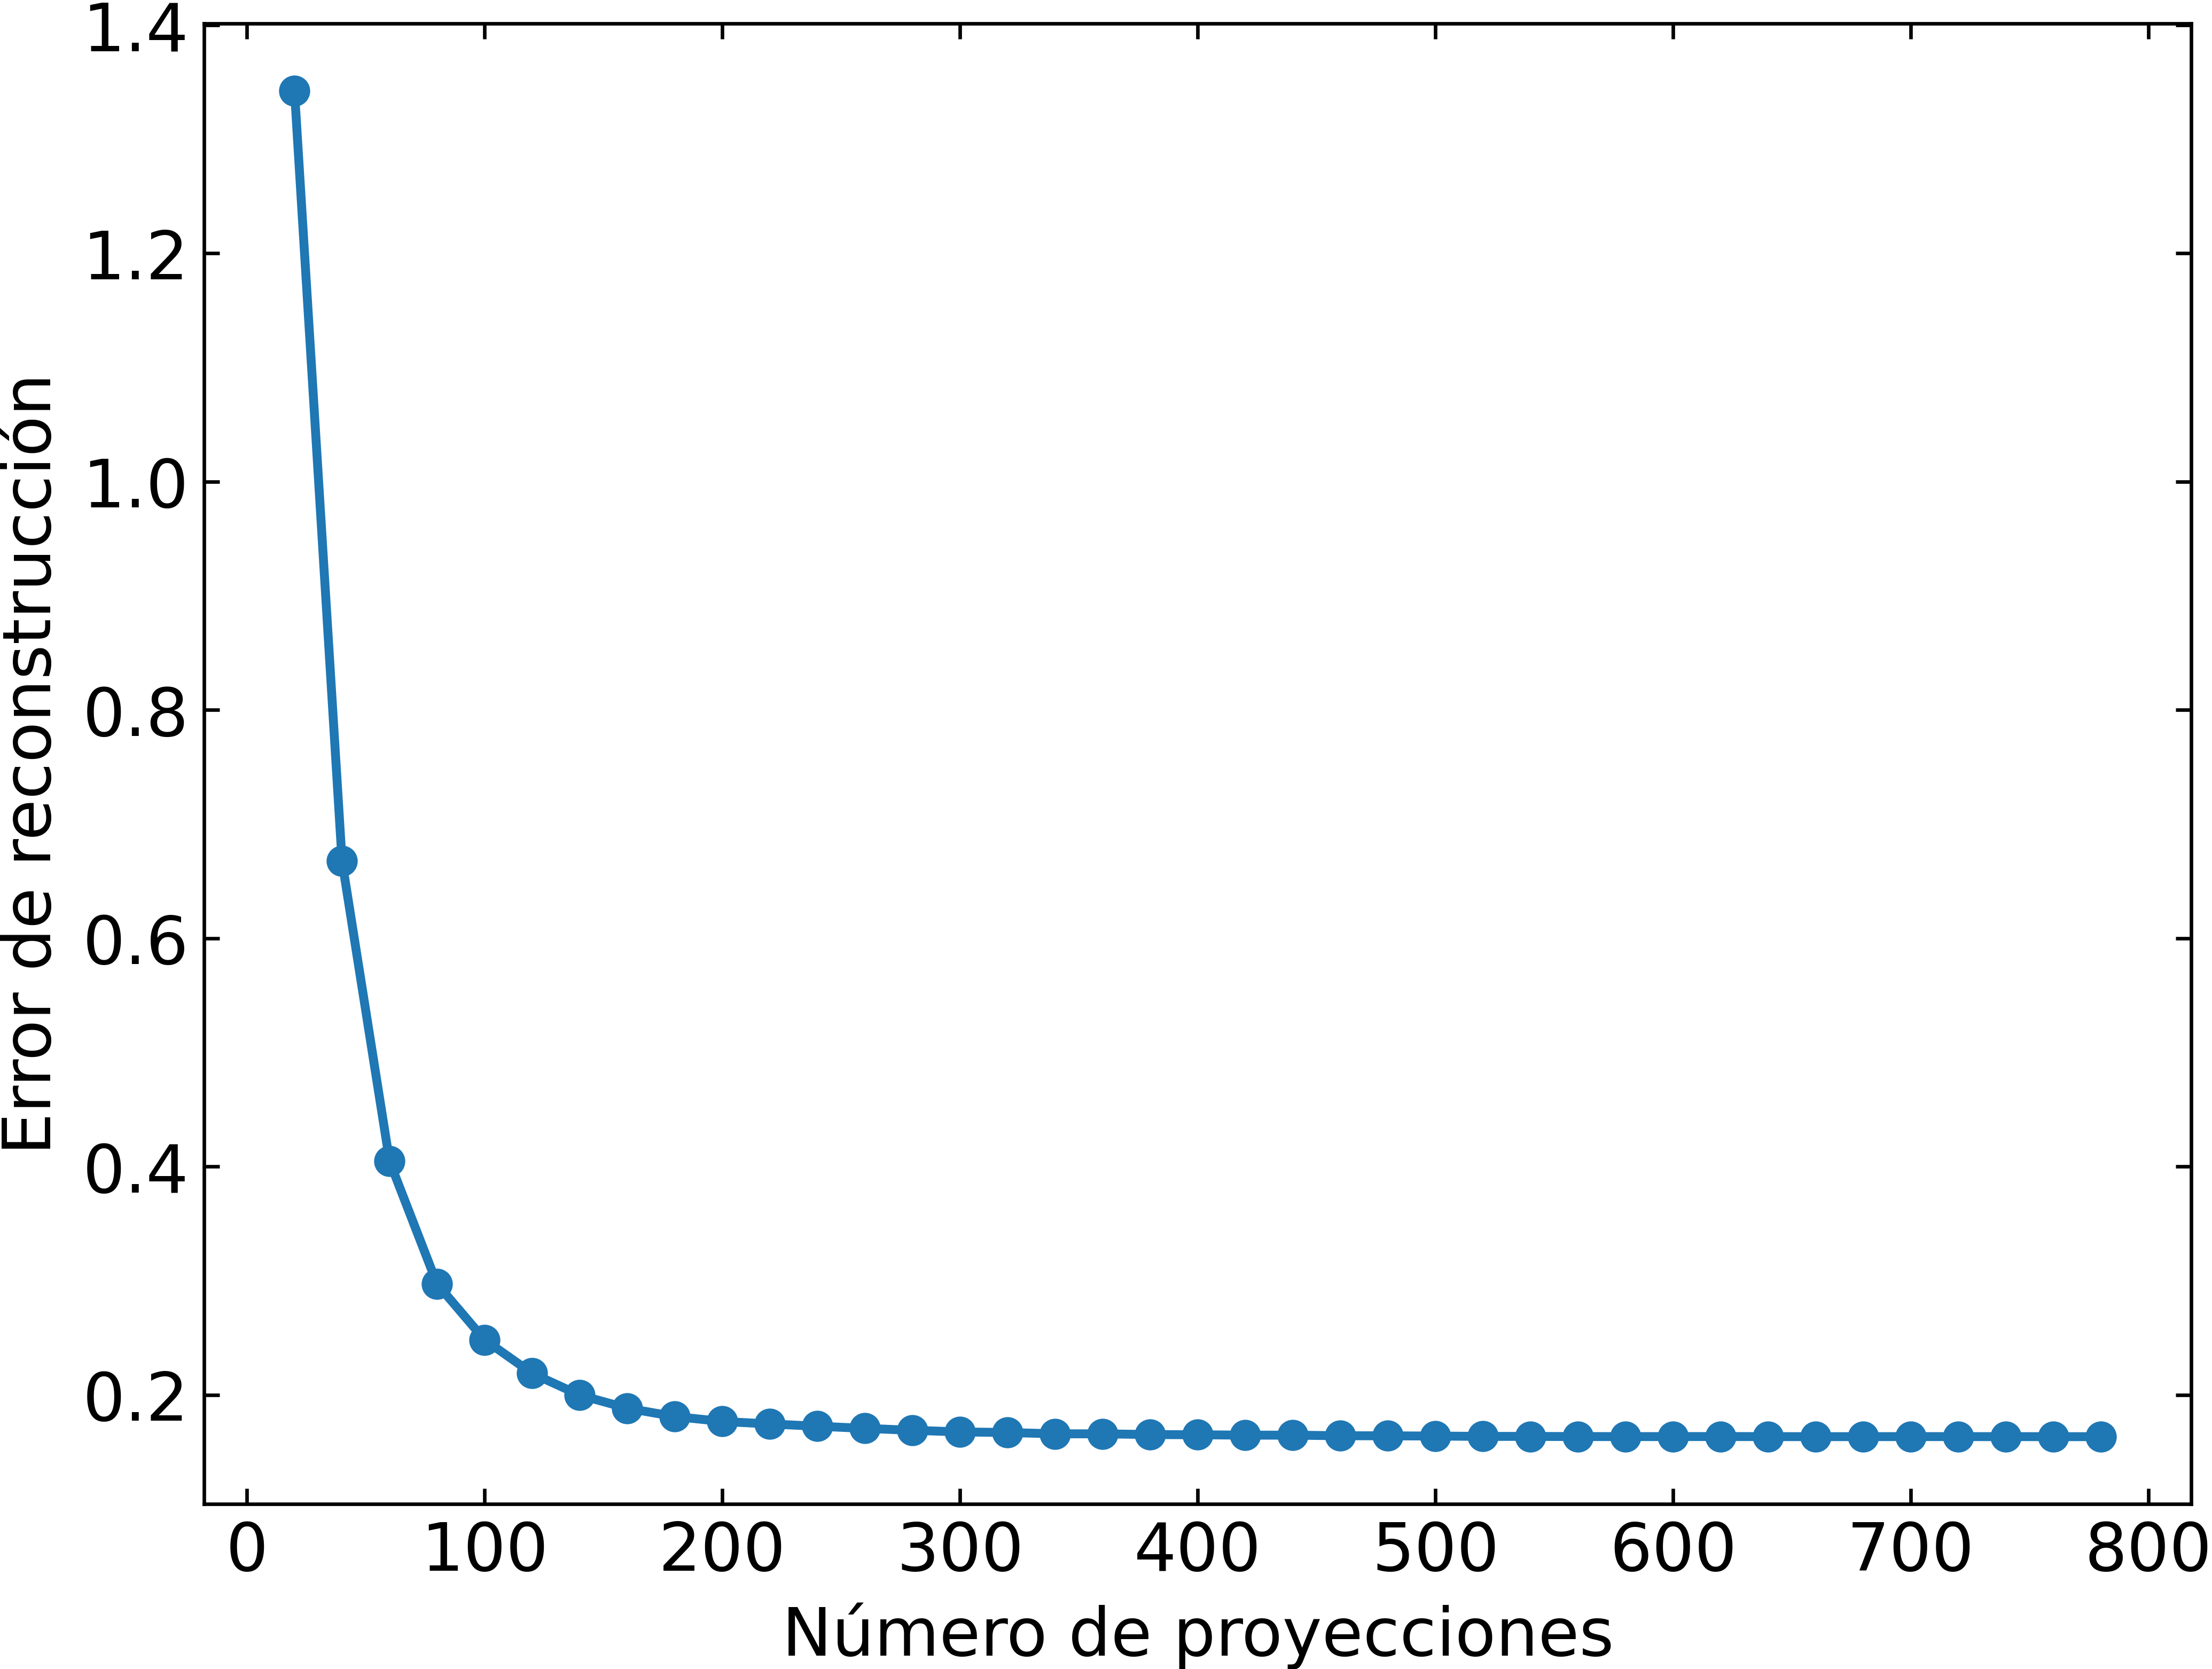
\includegraphics[width=\textwidth]{Figuras/error_vs_proyecciones.png}
           \caption{}
           \label{fig:err_proy}
        \end{subfigure}
        \begin{subfigure}[h]{0.32\linewidth}
         \centering
         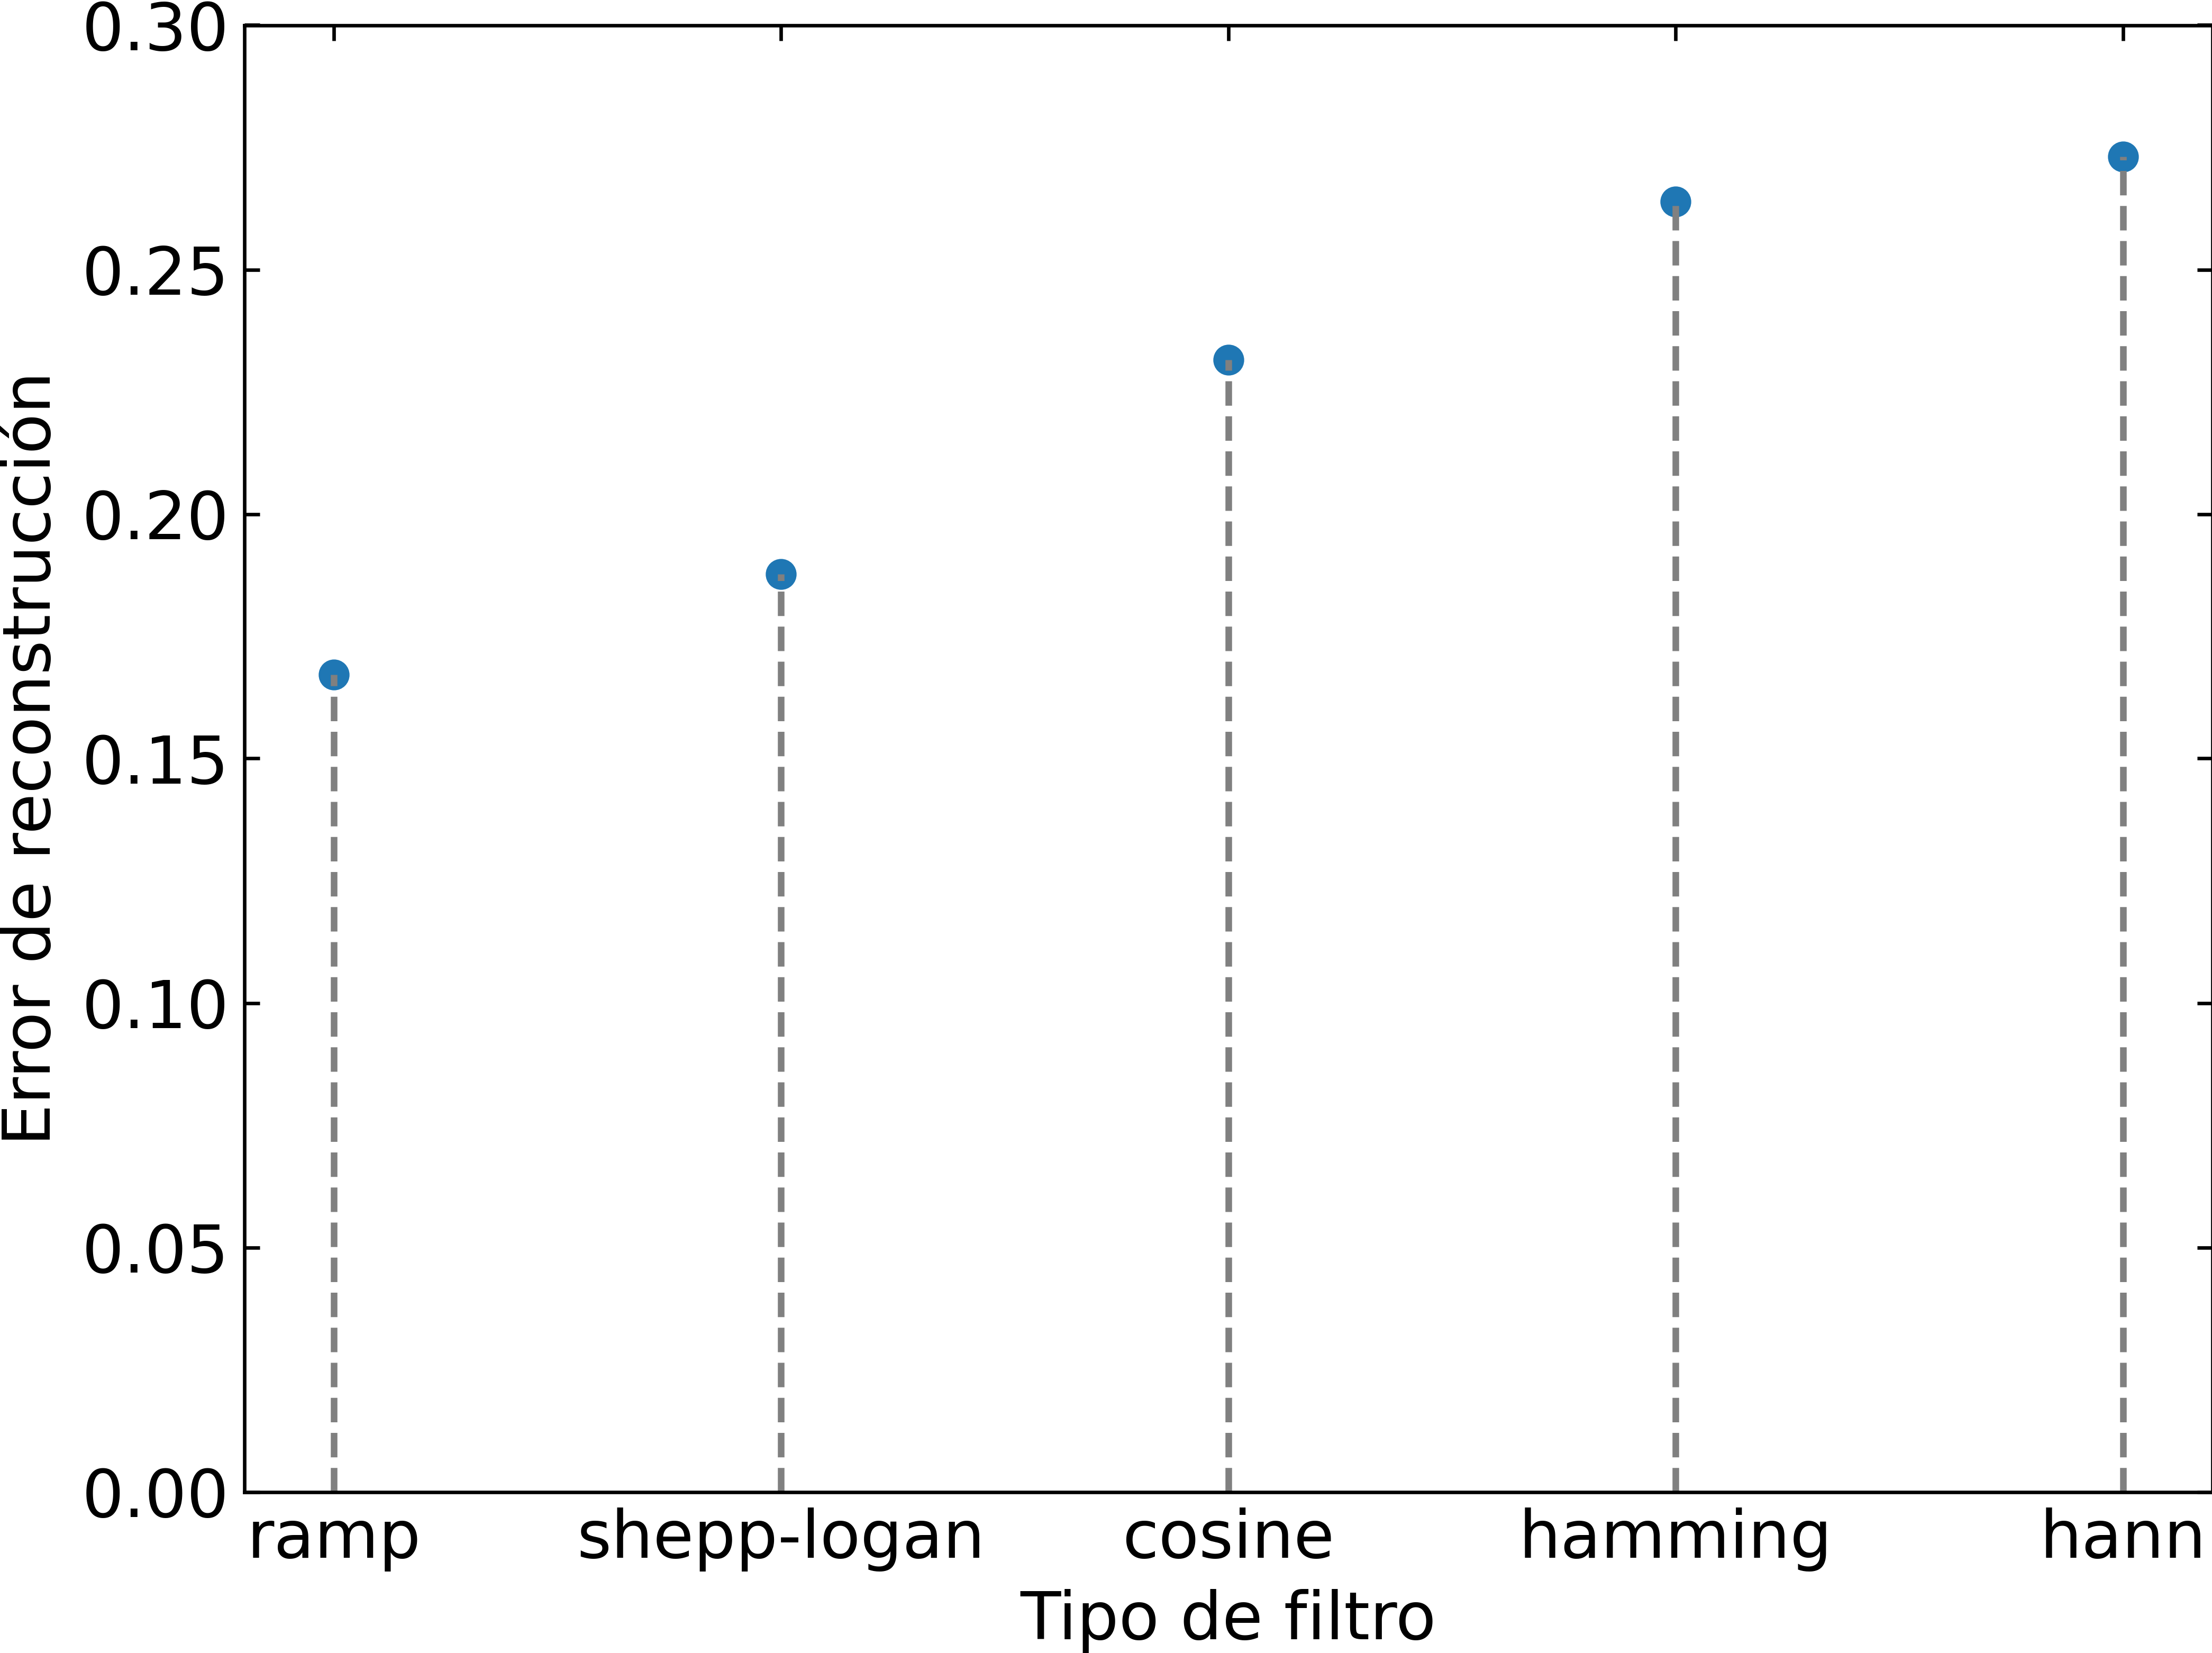
\includegraphics[width=\textwidth]{Figuras/error_vs_filters.png}
         \caption{}
         \label{fig:err_filtro}
      \end{subfigure}
   \caption{Errores de reconstrucción en función del número de detectores (a), número de proyecciones (b) y tipo de filtro (c).}
   \label{fig:err_vs_param}
\end{figure}

En general, se observa que al aumentar el número de detectores y proyecciones, el error de reconstrucción disminuye. Además, se observa que el filtro que mejor reconstrucción produce es el filtro rampa y que mayor error de reconstrucción da es el Hahn.

Para entender mejor que sucede con el error de reconstrucción en función del número de detectores y proyecciones, se generaron imágenes de reconstrucción con 25, 100, 200, 400 y 1000 detectores y 20, 100, 200, 400 y 800 proyecciones. Los resultados se muestran en la Fig. . Se observa que a medida que se aumenta el número de detectores y proyecciones, la reconstrucción se asemeja más al fantoma original y se producen menos artefactos.

\section{Sinograma de Shepp-Logan con ruido}

Se agregó ruido gaussiano al sinograma obtenido del fantoma Shepp-Logan con 367 detectores y 320 proyecciones (ver Fig. \ref{fig:SL_sinogram}) utilizando $\verb|python|$ en base al programa $\verb|radon-skimage.py|$ con ruido gaussiano con desvío igual al $10\%$ del valor máximo del sinograma. Posteriormente, se reconstruyó dicha imagen con retroproyección filtrada utilizando los filtros rampa, Hamming, Hanning y coseno. En la Fig. \ref{fig:noise_vs_filters} se muestran los resultados obtenidos. 

\begin{figure}[H]
   \centering
      \begin{subfigure}[h]{0.32\linewidth}
         \centering
         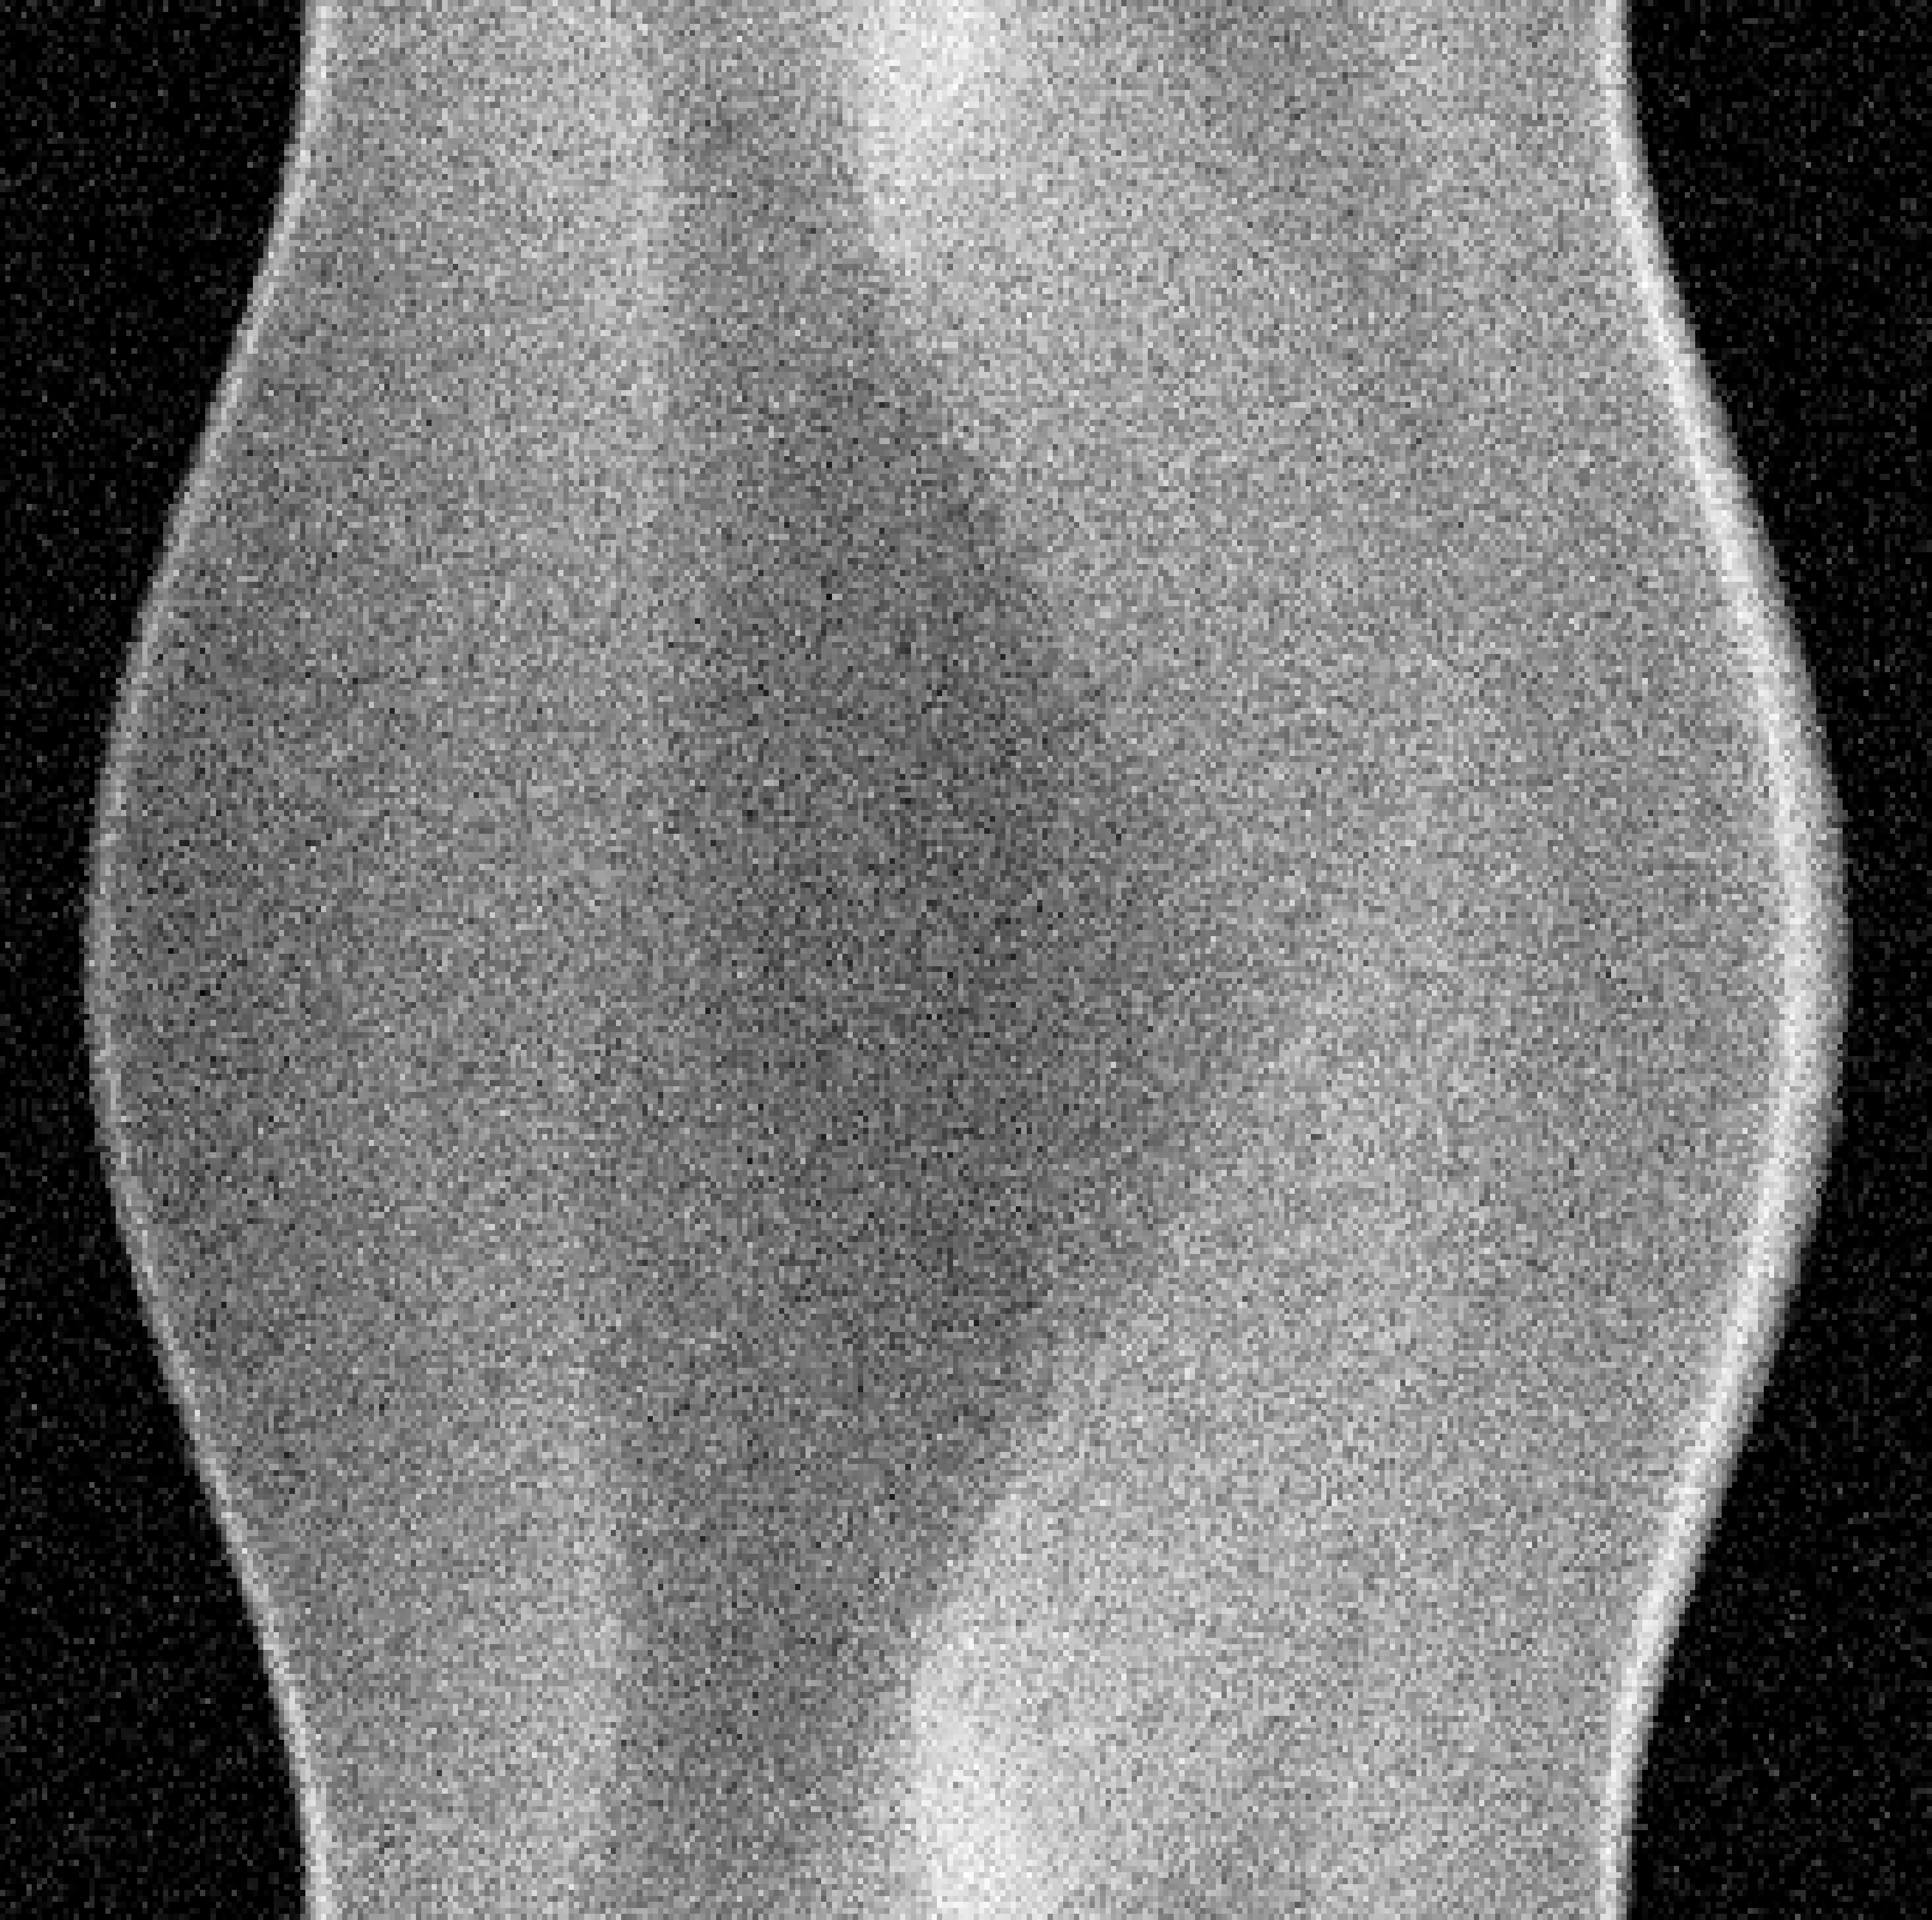
\includegraphics[width=\textwidth]{Figuras/sinograma_0.1.png}
         \caption{Sinograma con ruido.} 
         \label{fig:sinogram_0.1}
      \end{subfigure}
        \begin{subfigure}[h]{0.32\linewidth}
           \centering
           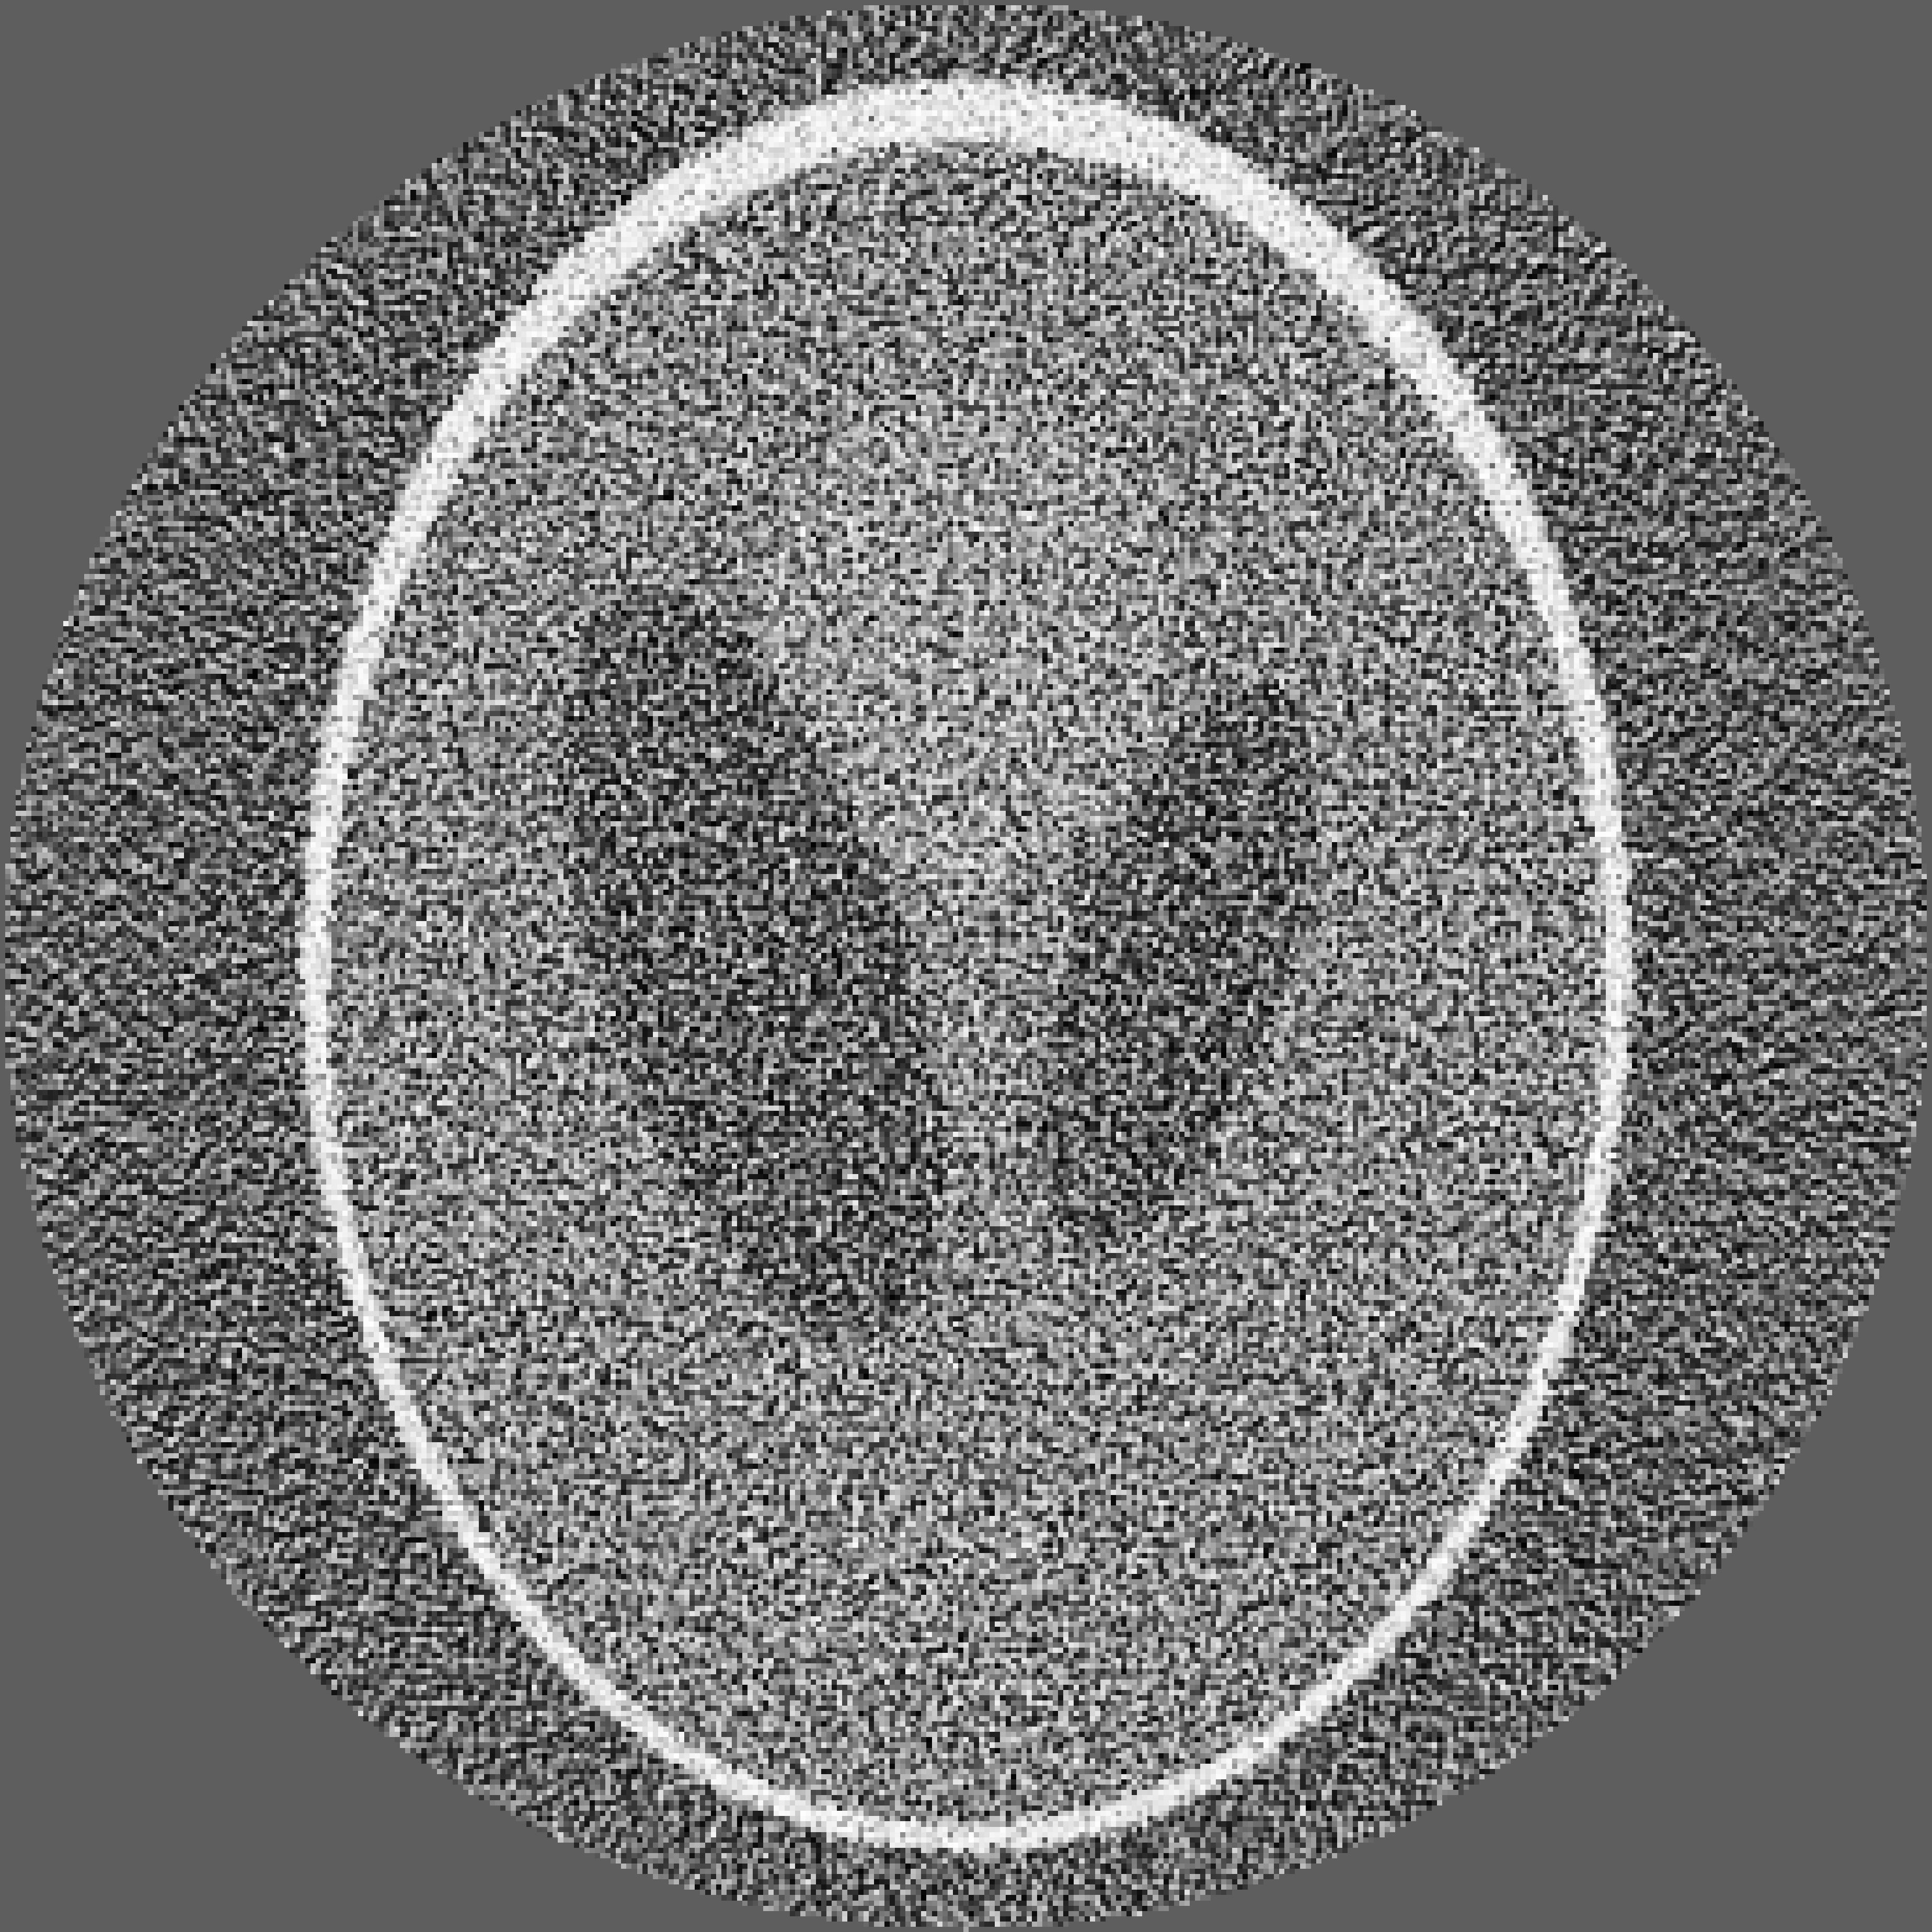
\includegraphics[width=\textwidth]{Figuras/reconstruction_ramp_EQ.png}
           \caption{Filtro rampa.} 
           \label{fig:noise_ramp}
        \end{subfigure}
        \begin{subfigure}[h]{0.32\linewidth}
           \centering
           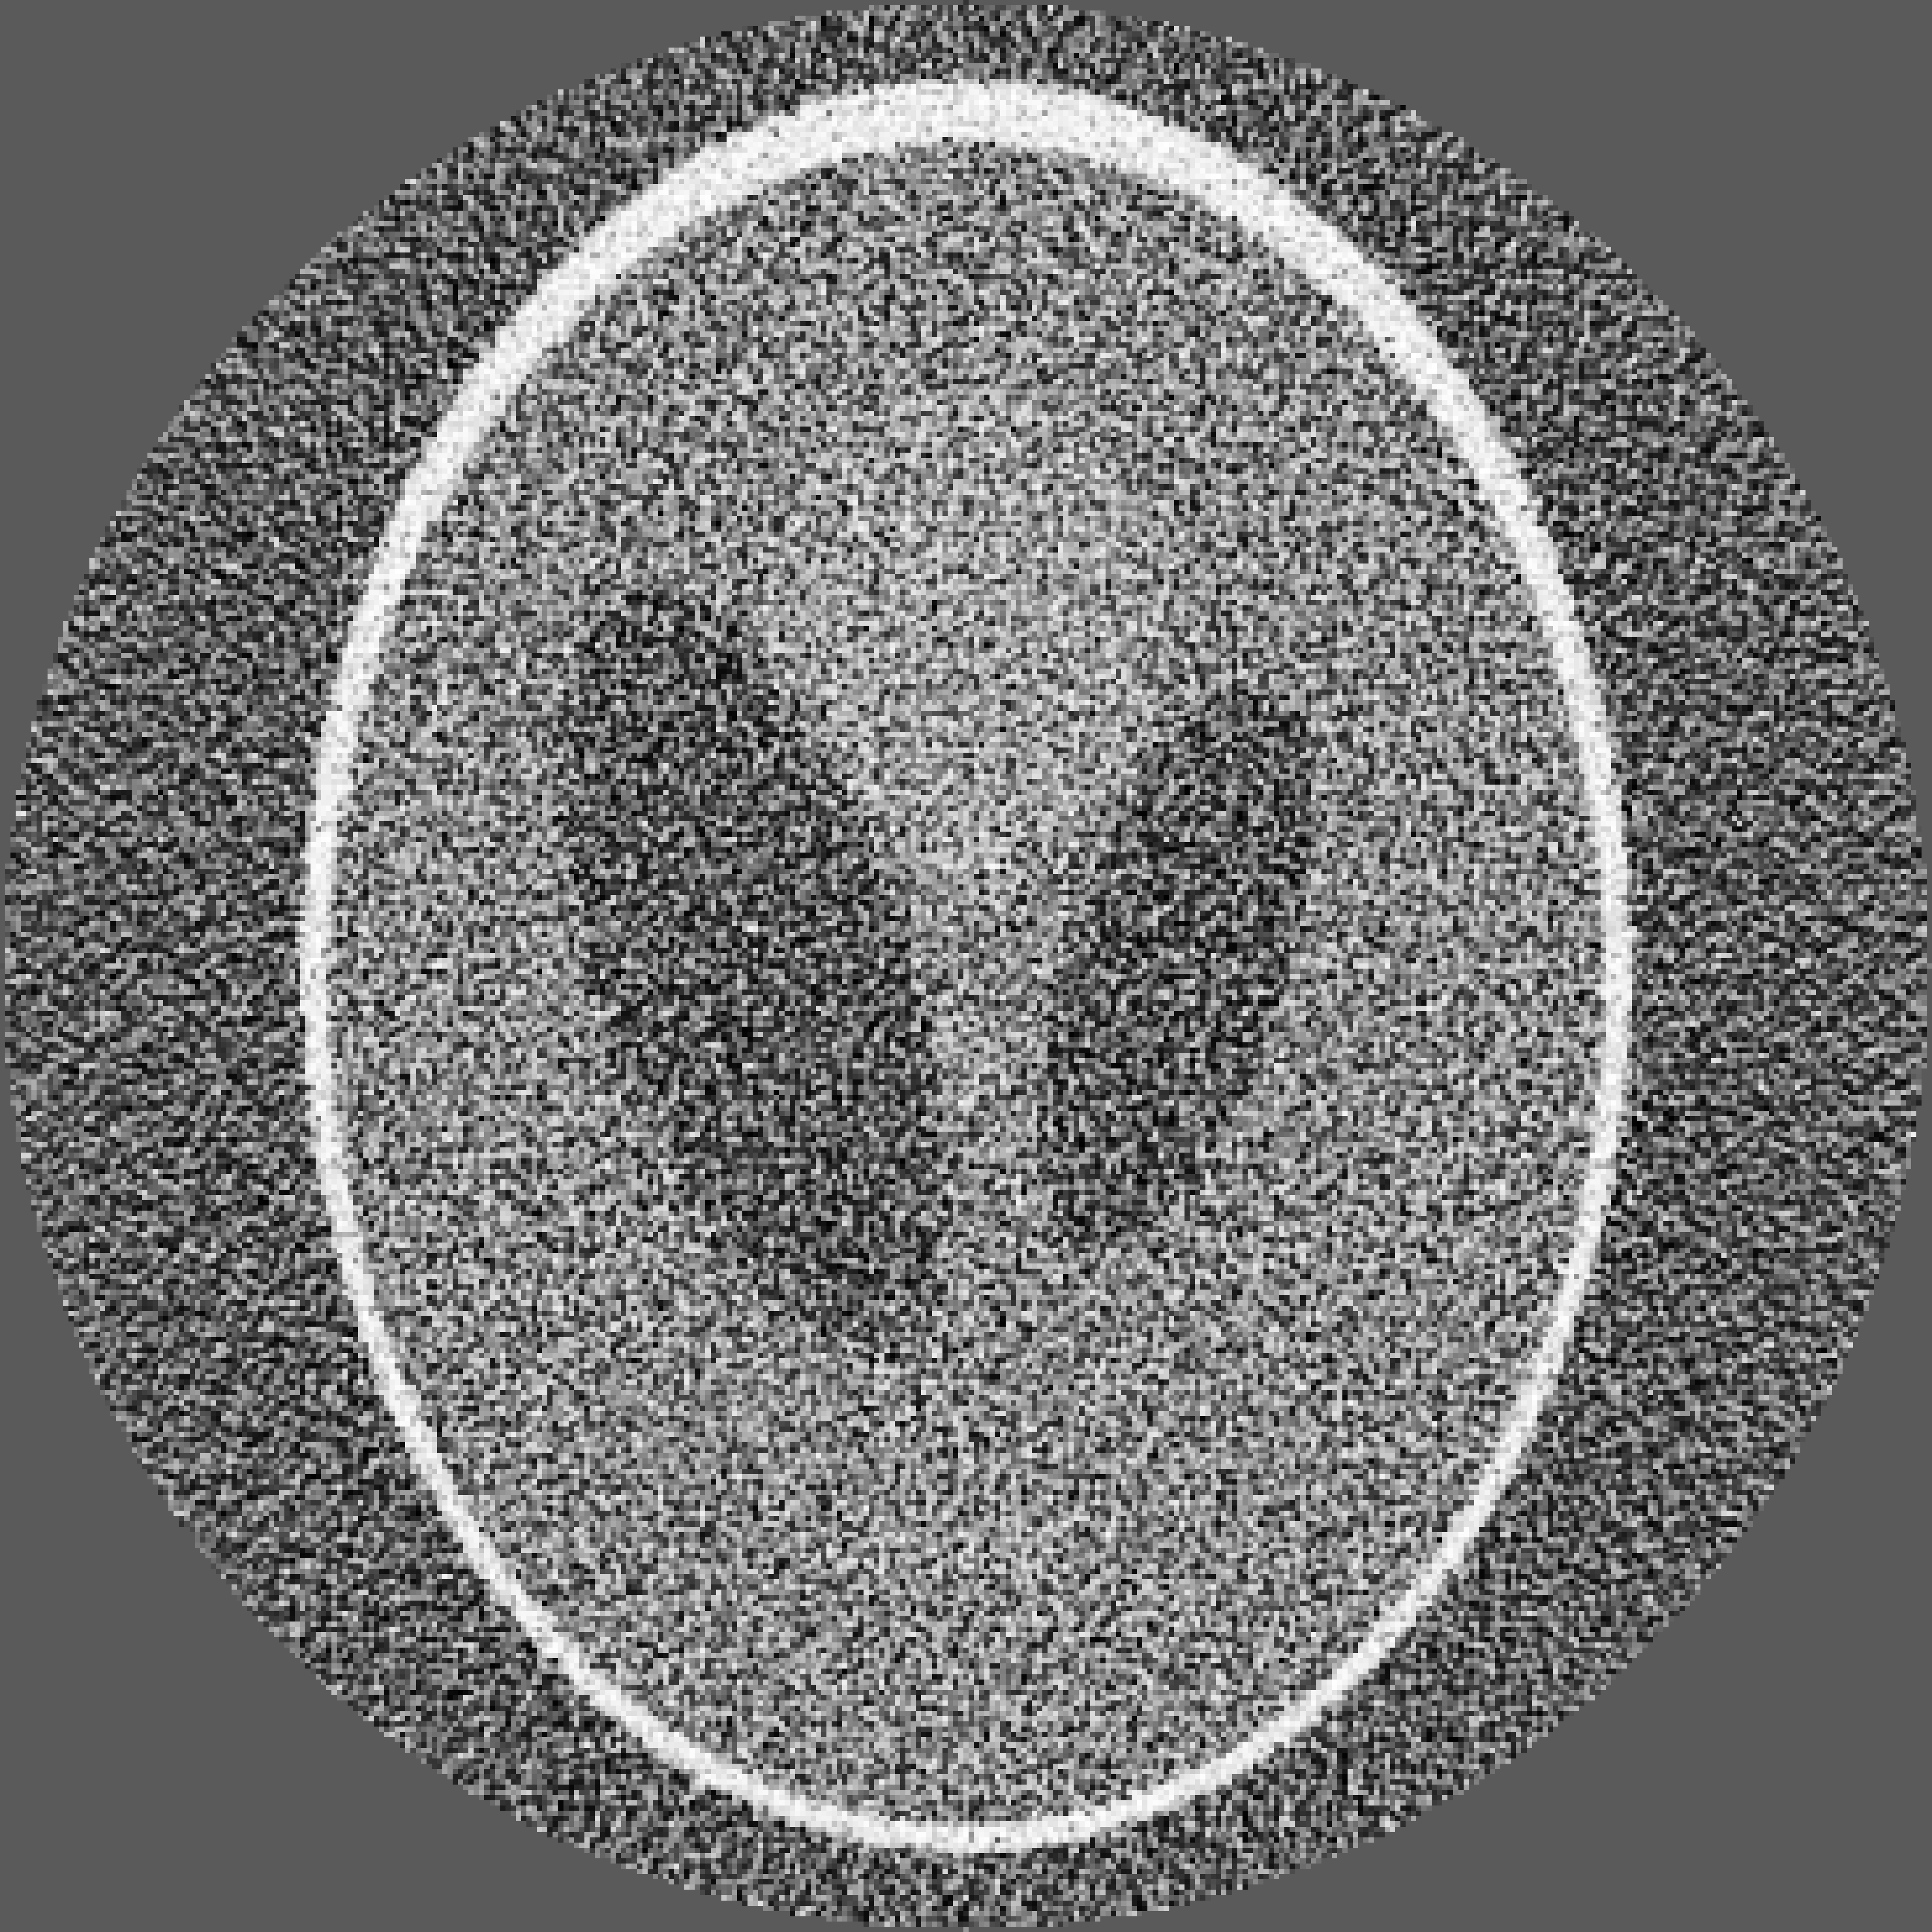
\includegraphics[width=\textwidth]{Figuras/reconstruction_shepp-logan_EQ.png}
           \caption{Filtro Shepp-Logan.}
           \label{fig:noise_shepp}
        \end{subfigure}
        \begin{subfigure}[h]{0.32\linewidth}
            \centering
            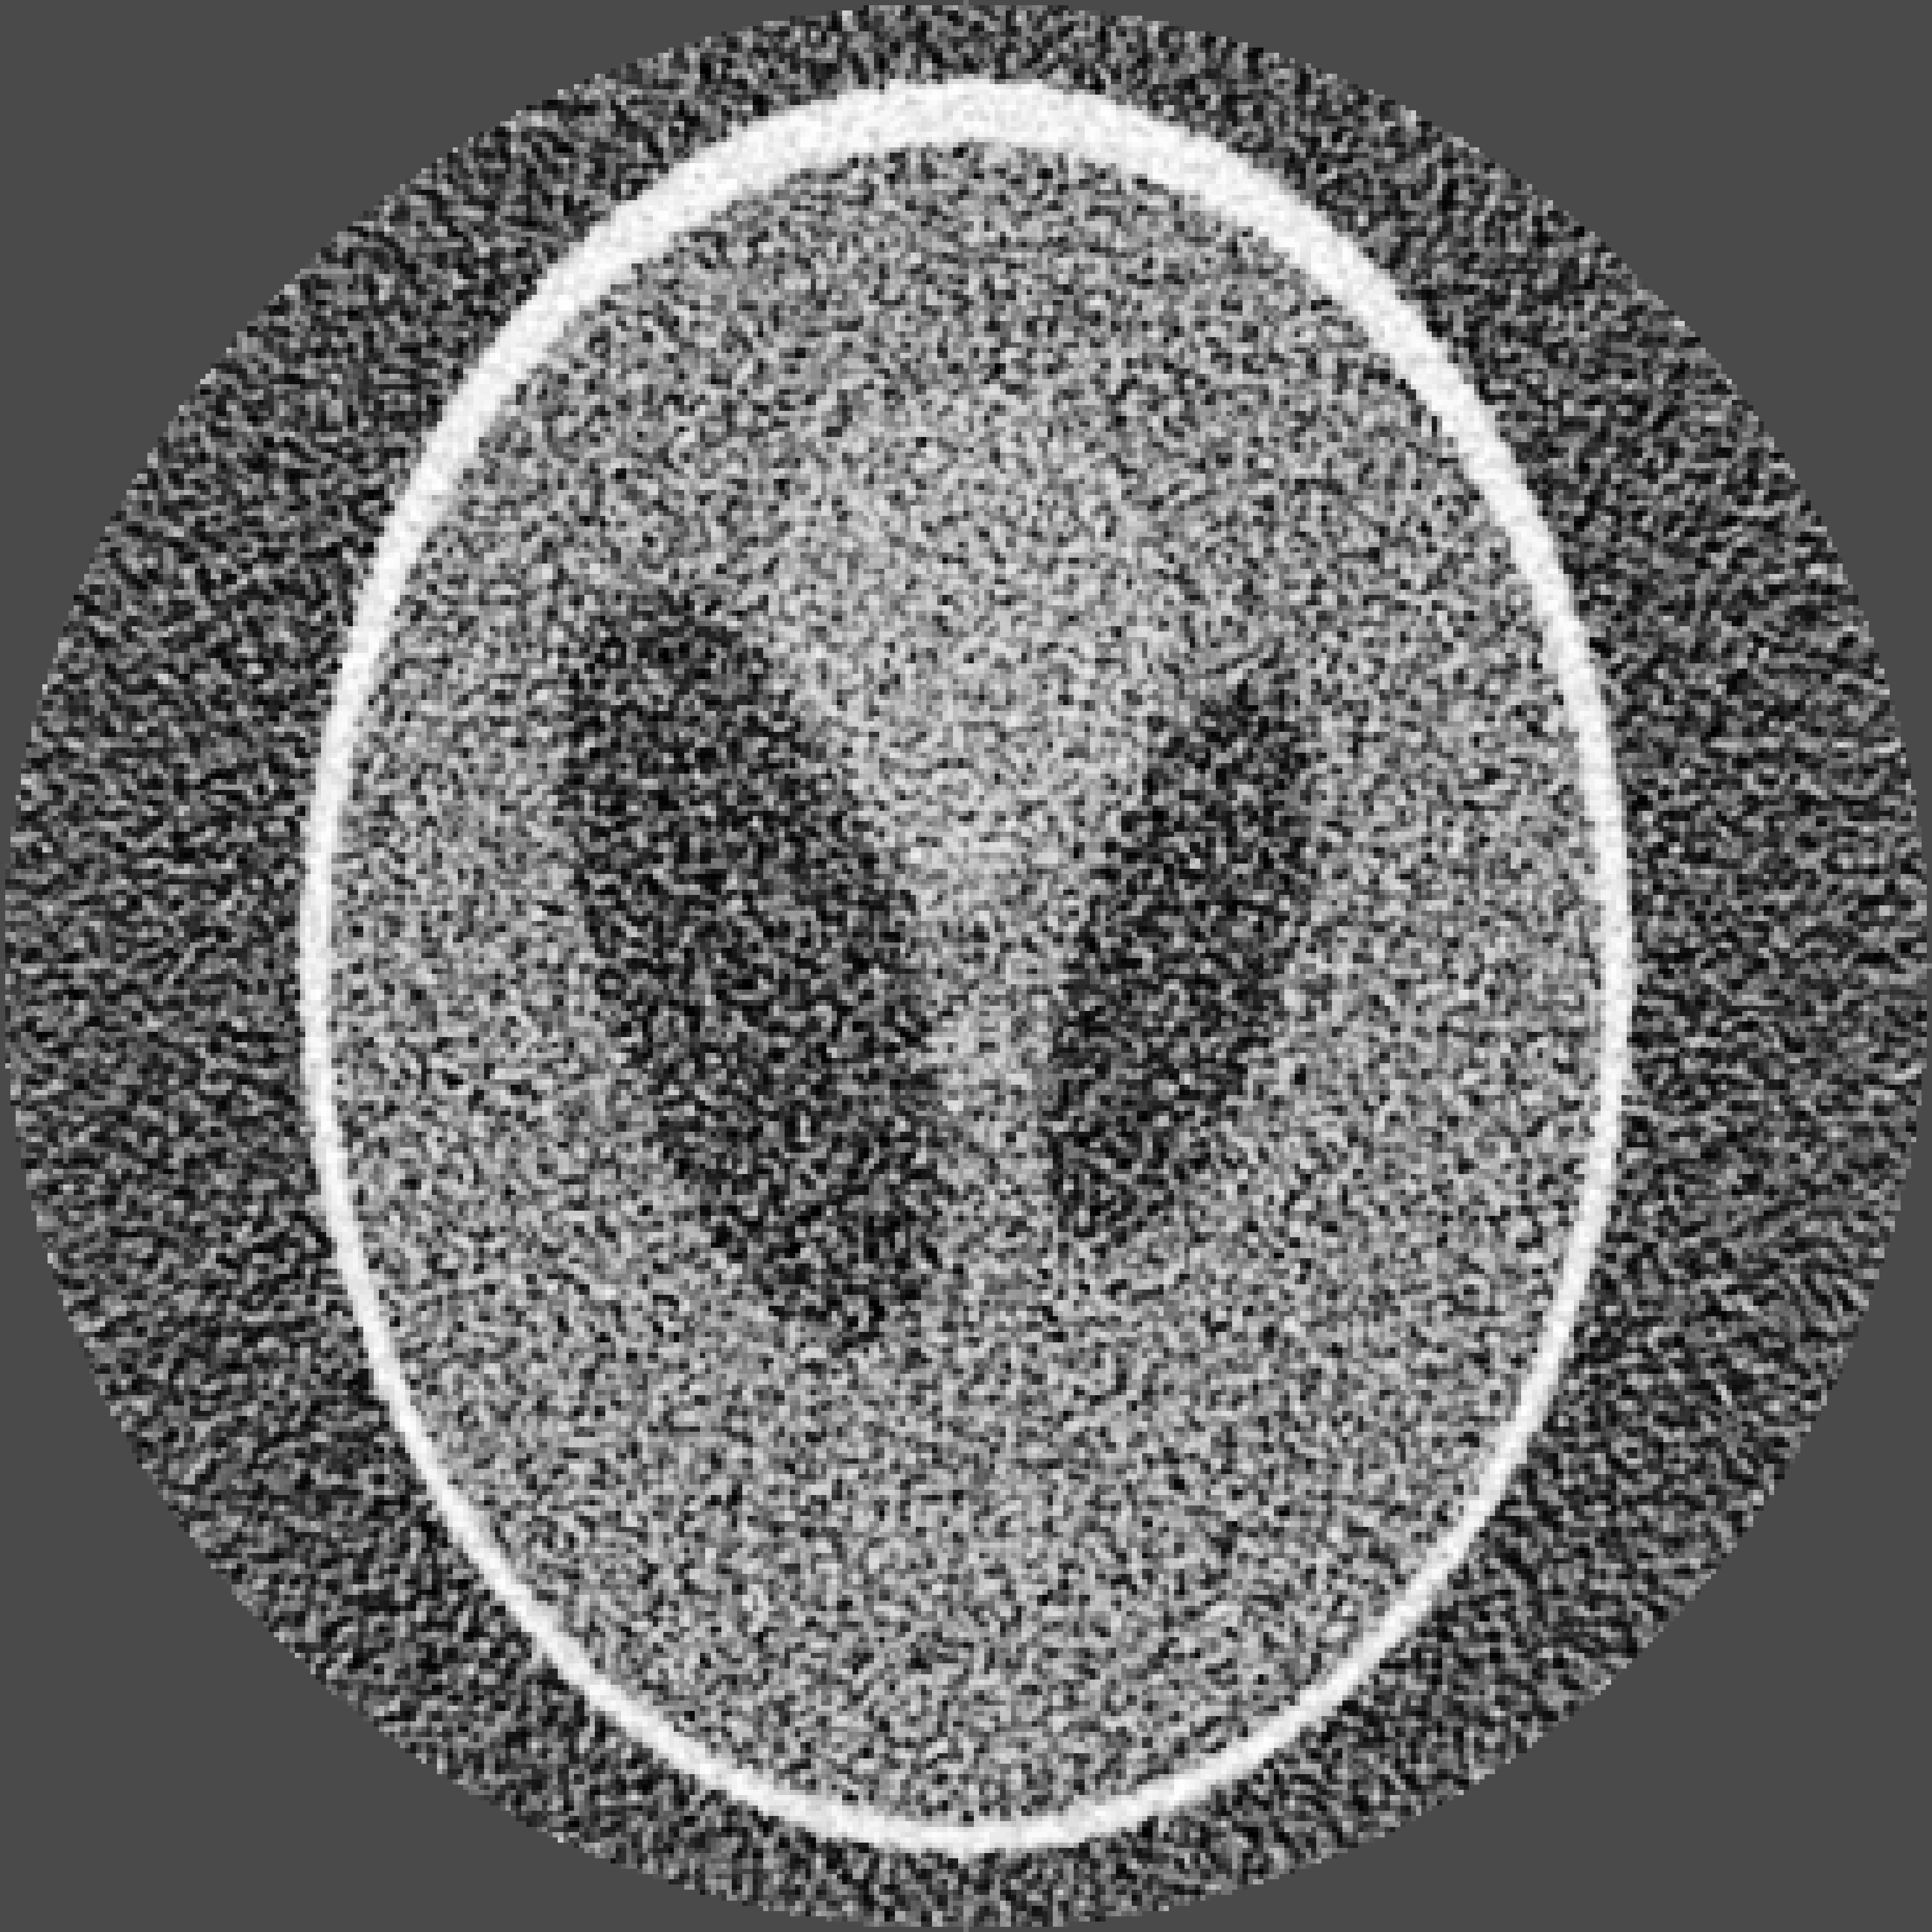
\includegraphics[width=\textwidth]{Figuras/reconstruction_cosine_EQ.png}
            \caption{Filtro coseno.}
         \label{fig:noise_coseno}
       \end{subfigure}
         \begin{subfigure}[h]{0.32\linewidth}
            \centering
            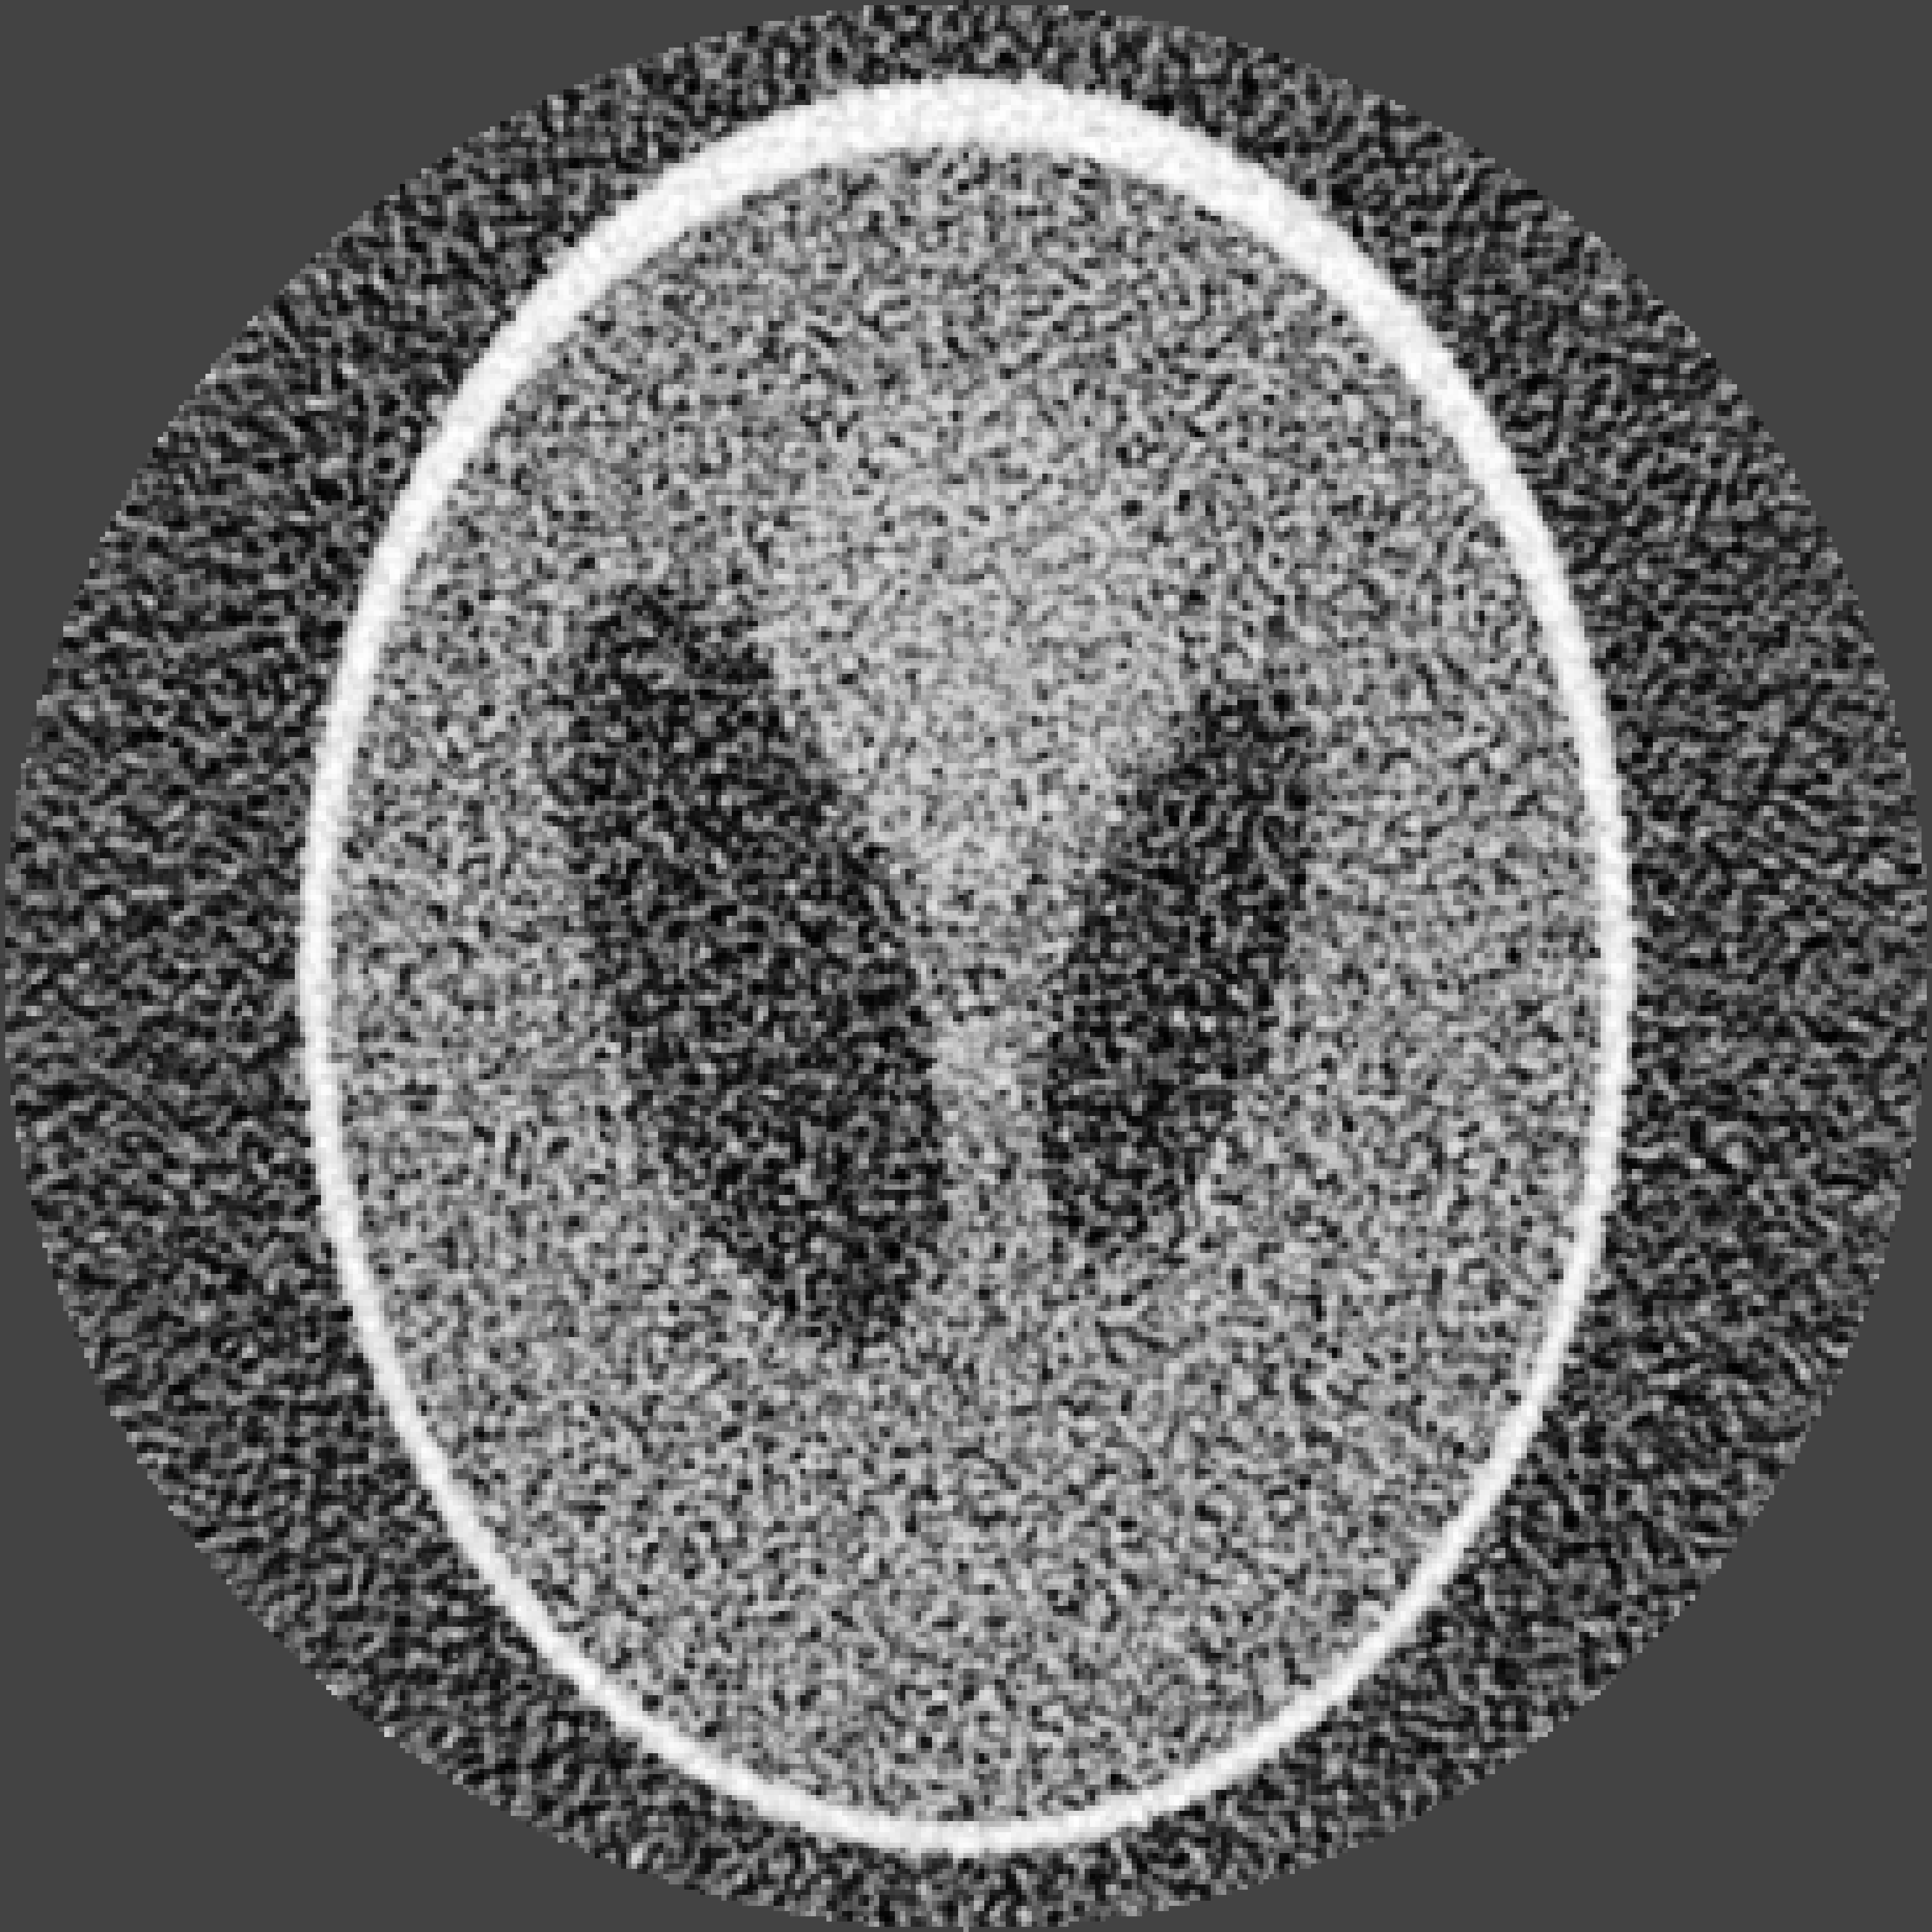
\includegraphics[width=\textwidth]{Figuras/reconstruction_hamming_EQ.png}
            \caption{Filtro Hamming.}
            \label{fig:noise_hamming}
         \end{subfigure}
         \begin{subfigure}[h]{0.32\linewidth}
            \centering
            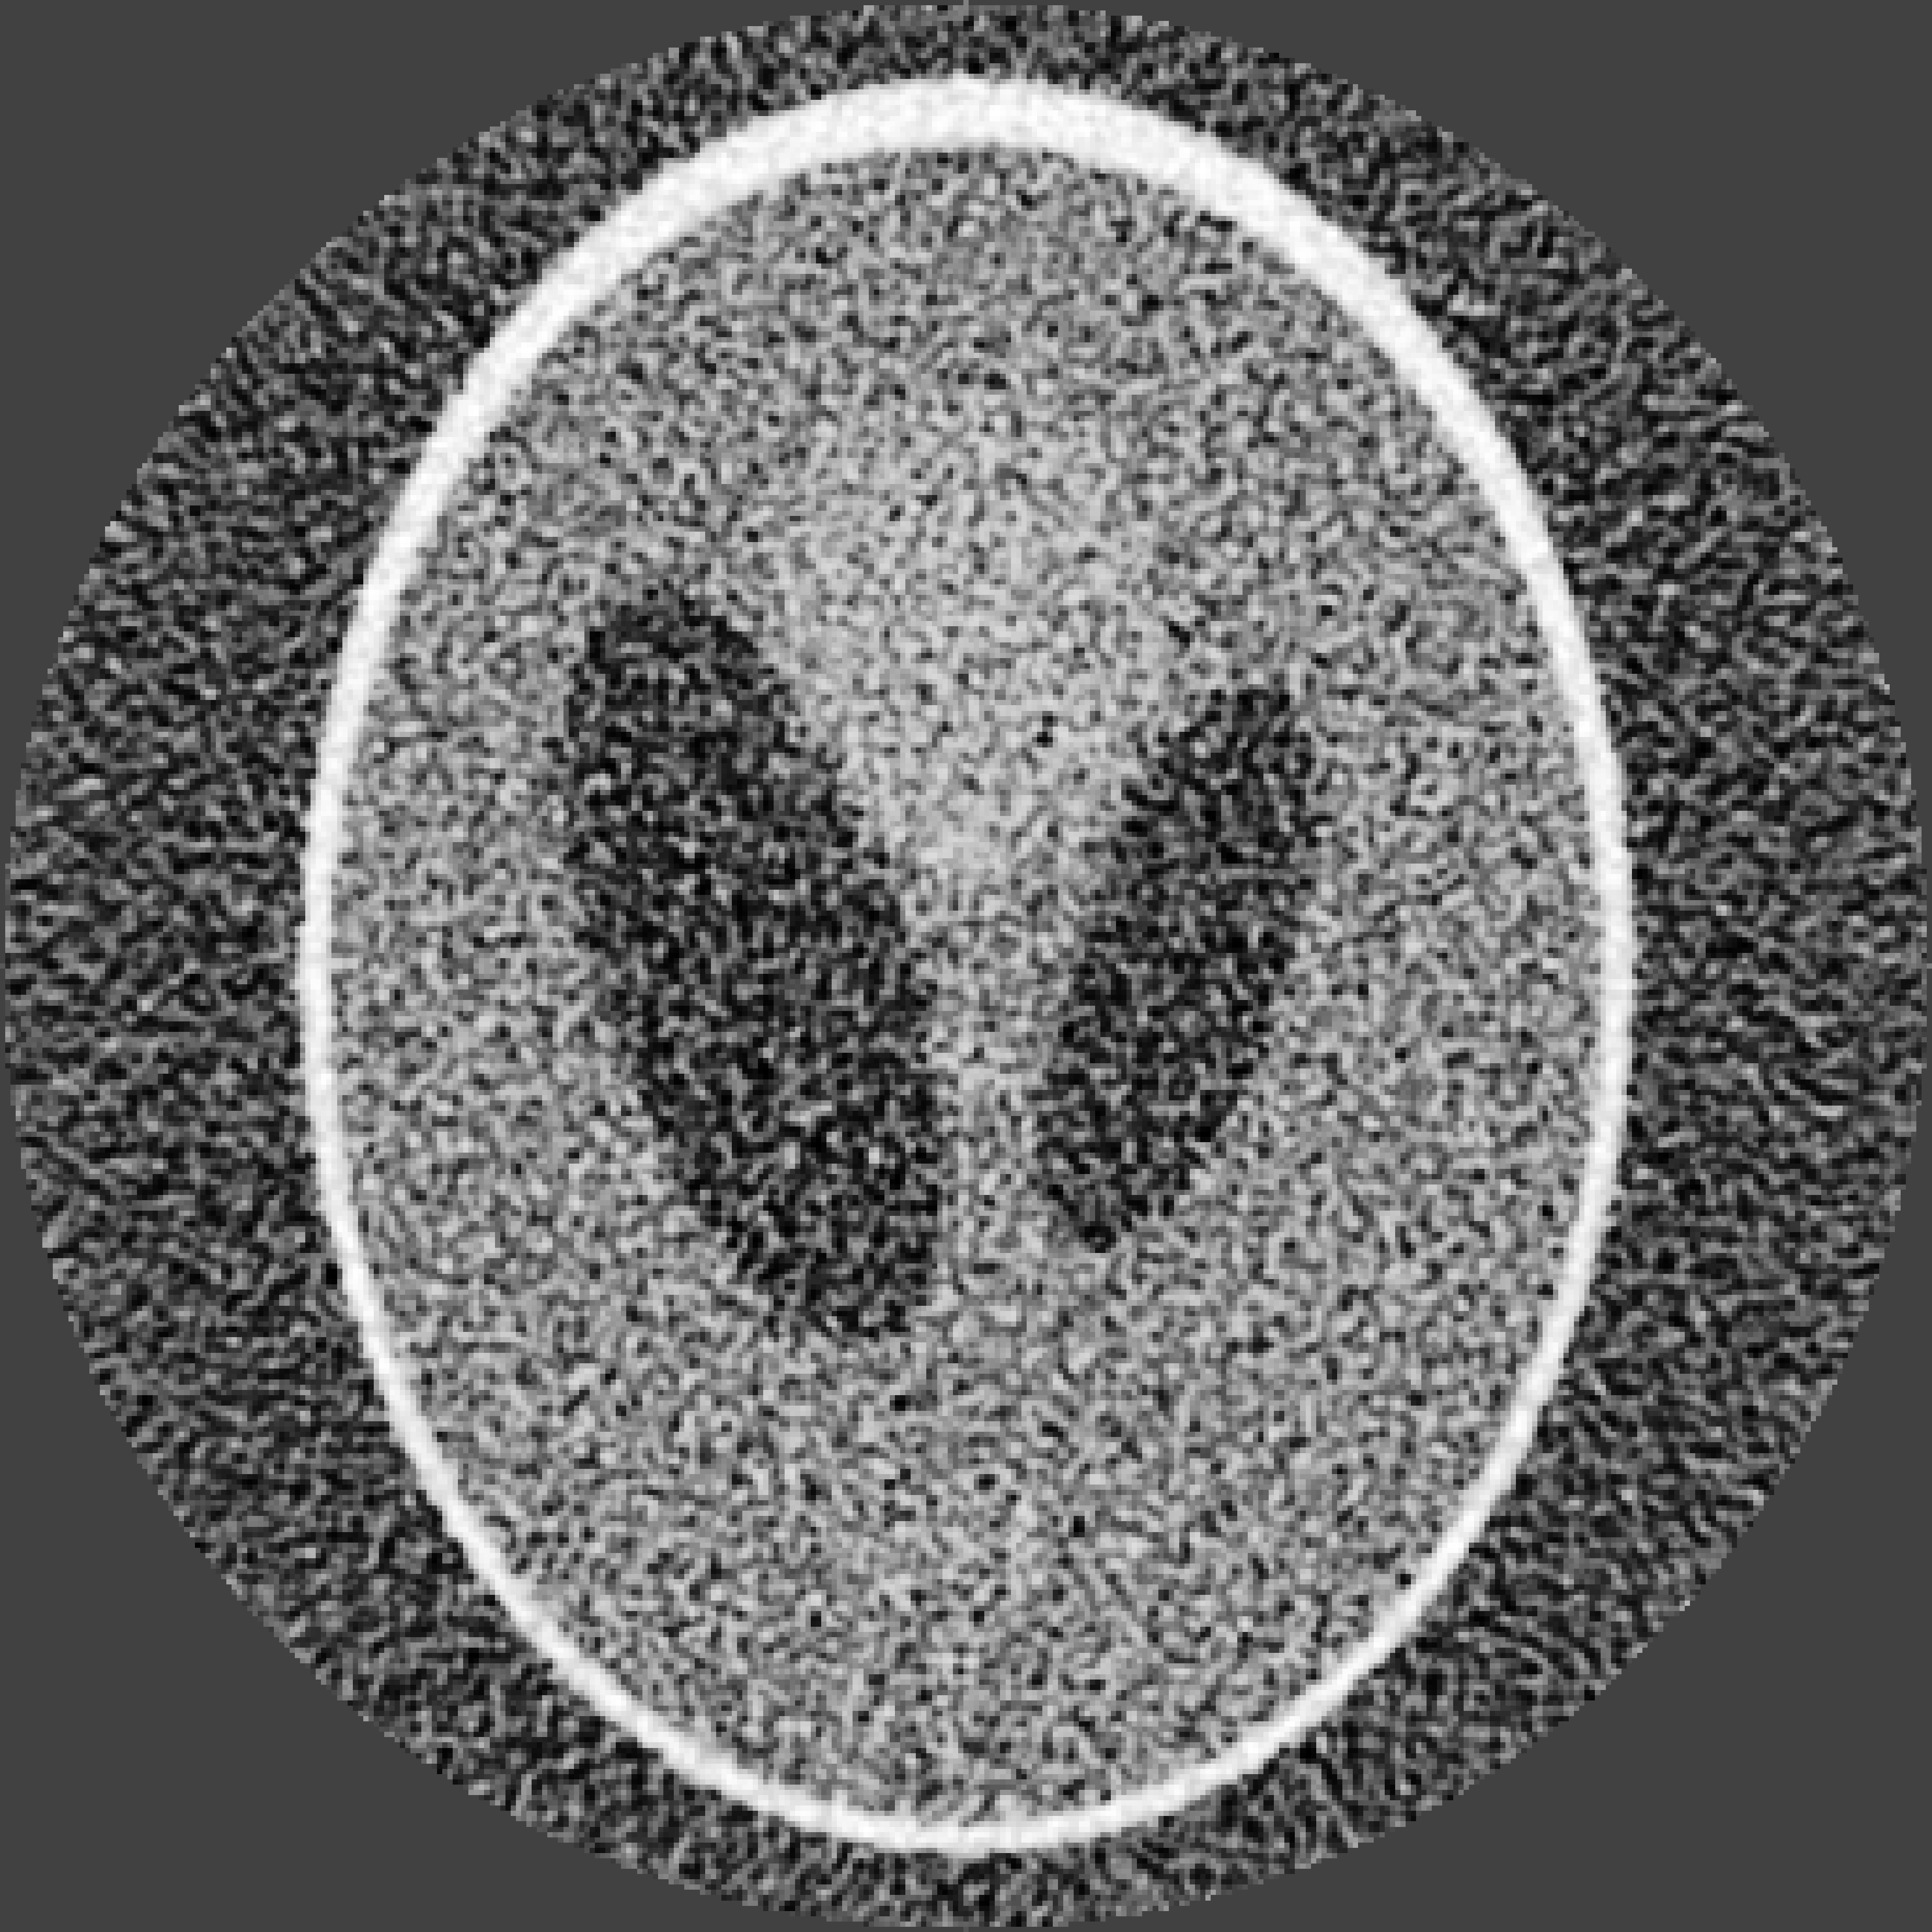
\includegraphics[width=\textwidth]{Figuras/reconstruction_hann_EQ.png}
            \caption{Filtro Hahn.}
            \label{fig:noise_hahn}
      \end{subfigure}
   \caption{Retroproyección filtrada del sinograma con ruido (a), número de proyecciones (b) y tipo de filtro (c)}
   \label{fig:noise_vs_filters}
\end{figure}

\begin{figure}[H]
   \centering
         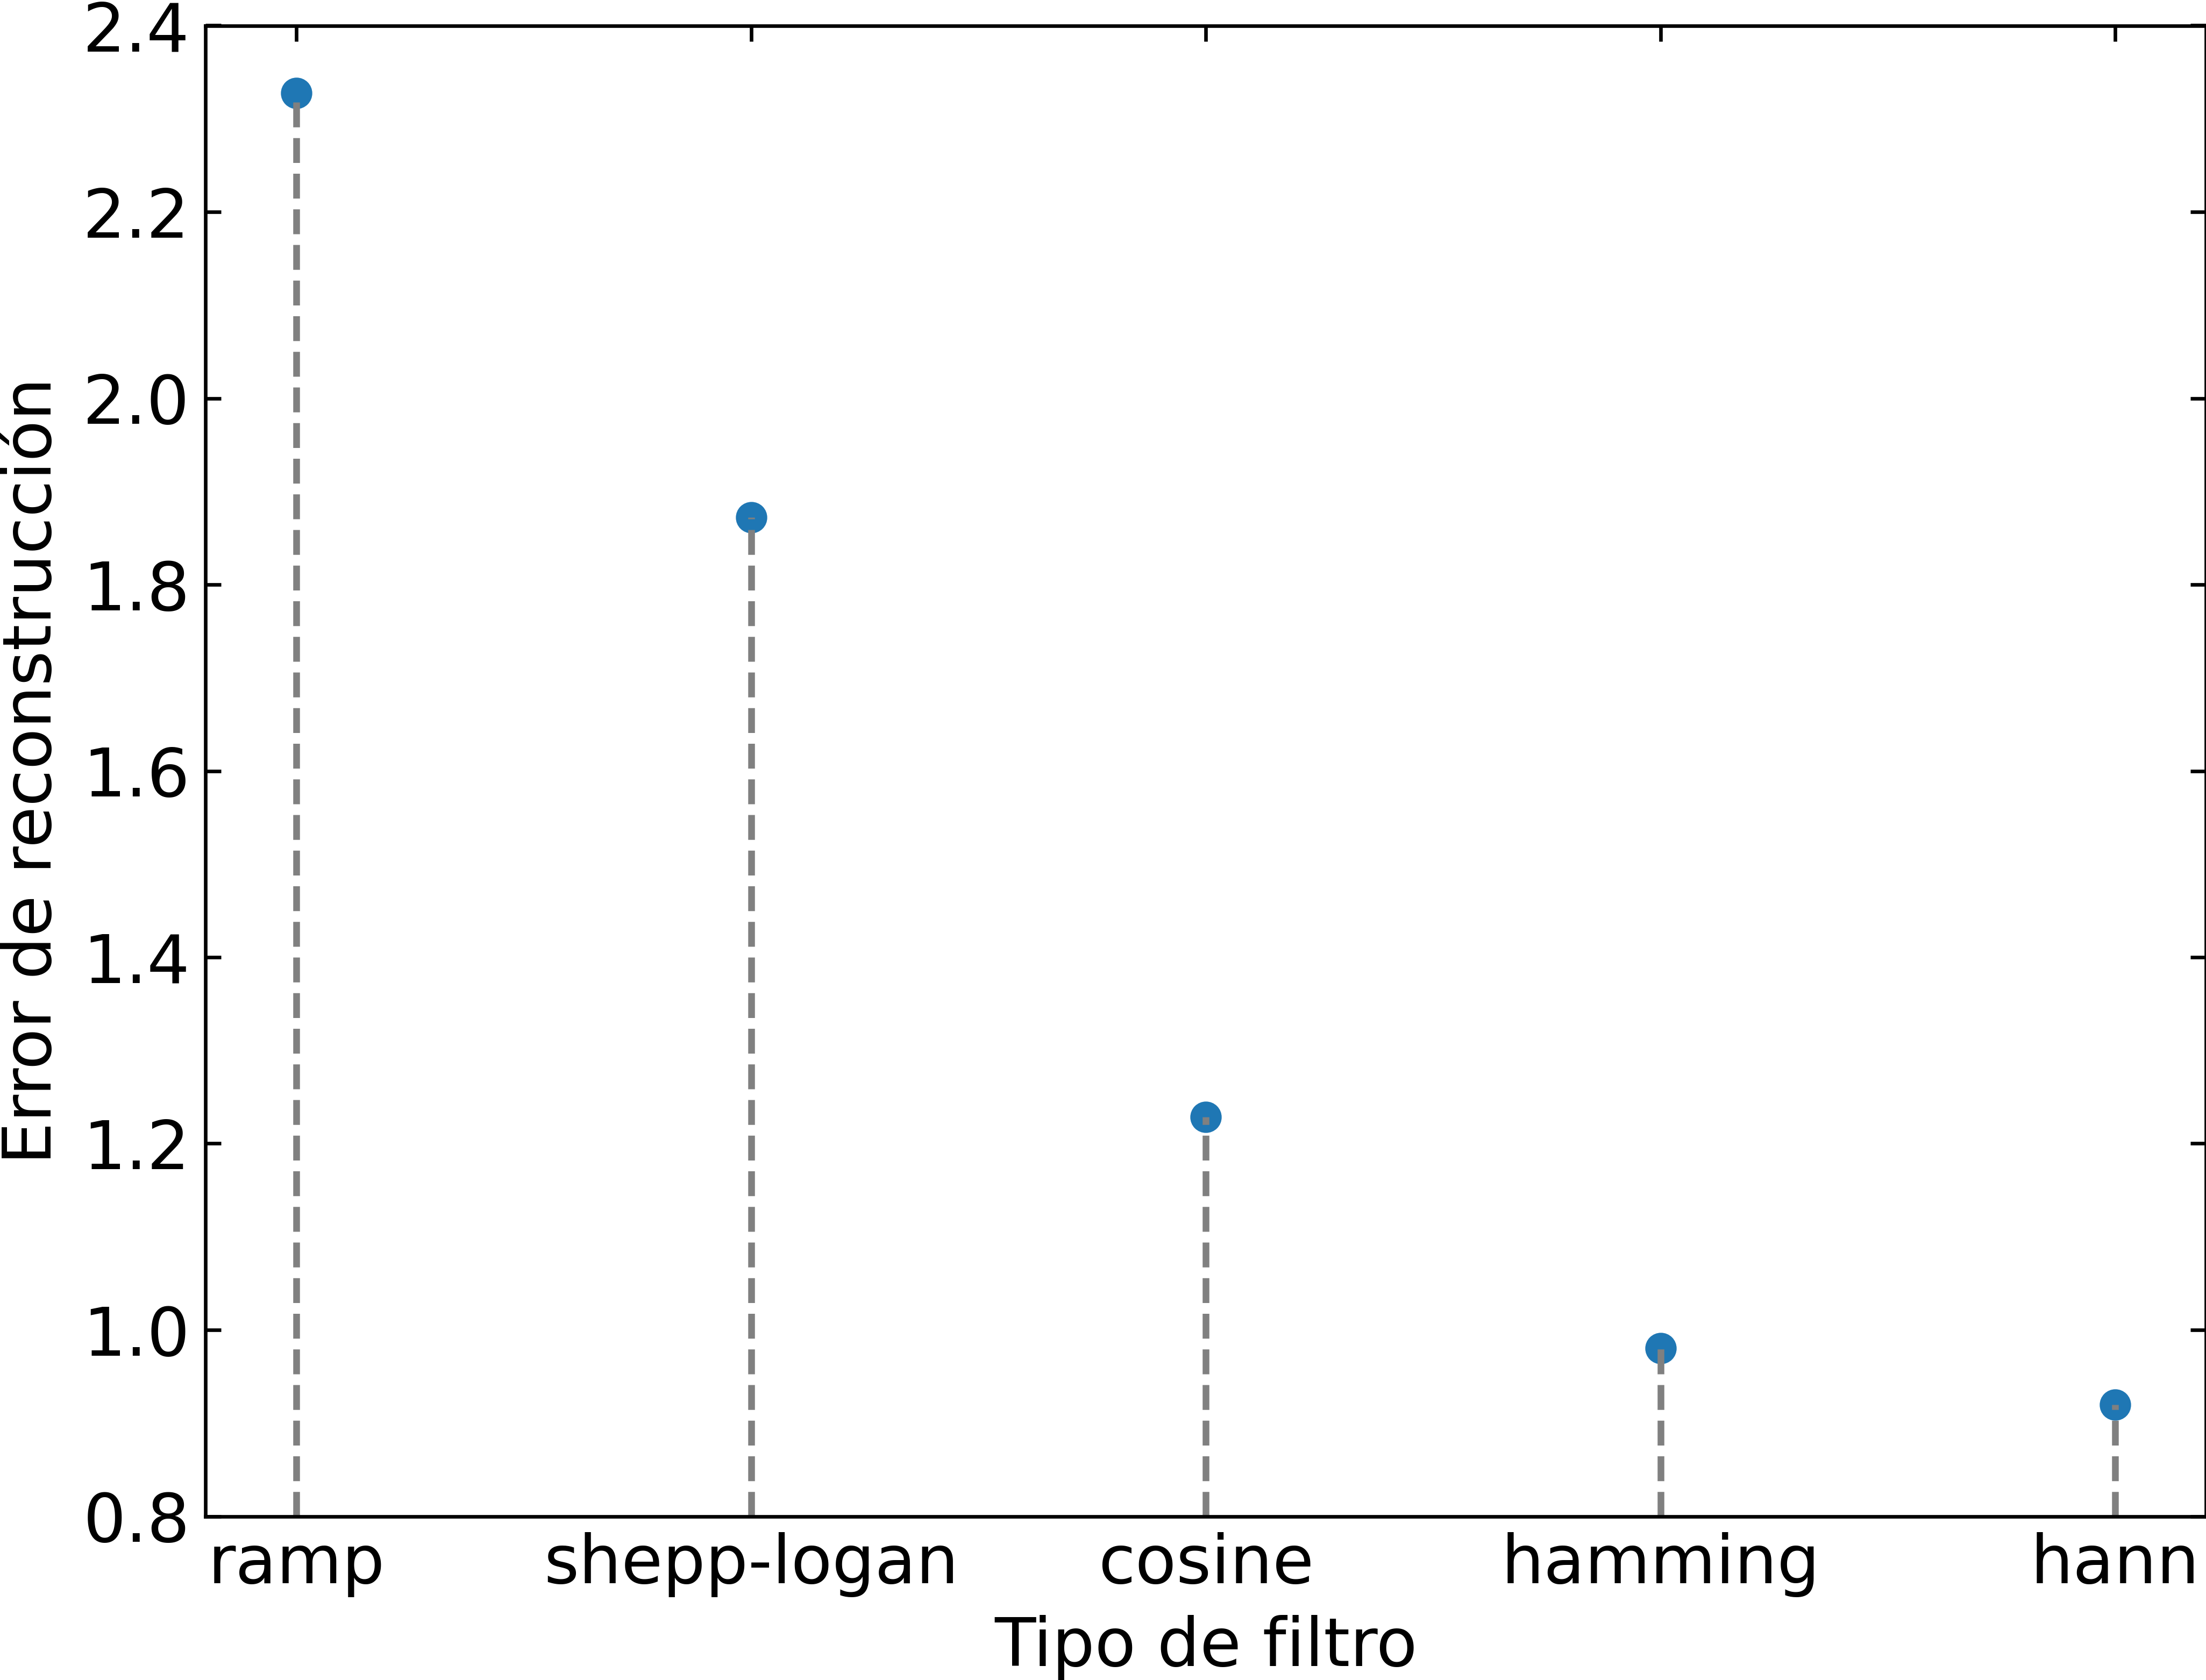
\includegraphics[width=0.5\textwidth]{Figuras/error_vs_filters_noise.png}
   \caption{Error de reconstrucción para cada filtro aplicado sobre el sinograma con ruido.}
   \label{fig:filters_noise}
\end{figure}

\section{Proyecciones paralelas de un círculo}

Utilizando la libreria $\verb|OpenCV|$ de Python se creó una imagen de $100\times100$ negra con un círculo blanco de radio $3$ pixels centrado en el medio de la imagen como se muestra en la Fig. \ref{fig:sinograma_circulo}.Utilizando el programa provisto $\verb|radon-skimage.py|$ se generó un sinograma de esta imagen con 100 detectores y $8,16,32,64$ proyecciones. 


Los resultados se encuentran en la Fig. \ref{fig:retroproyeccion_circulo}.

\begin{figure}[H]
   \centering
         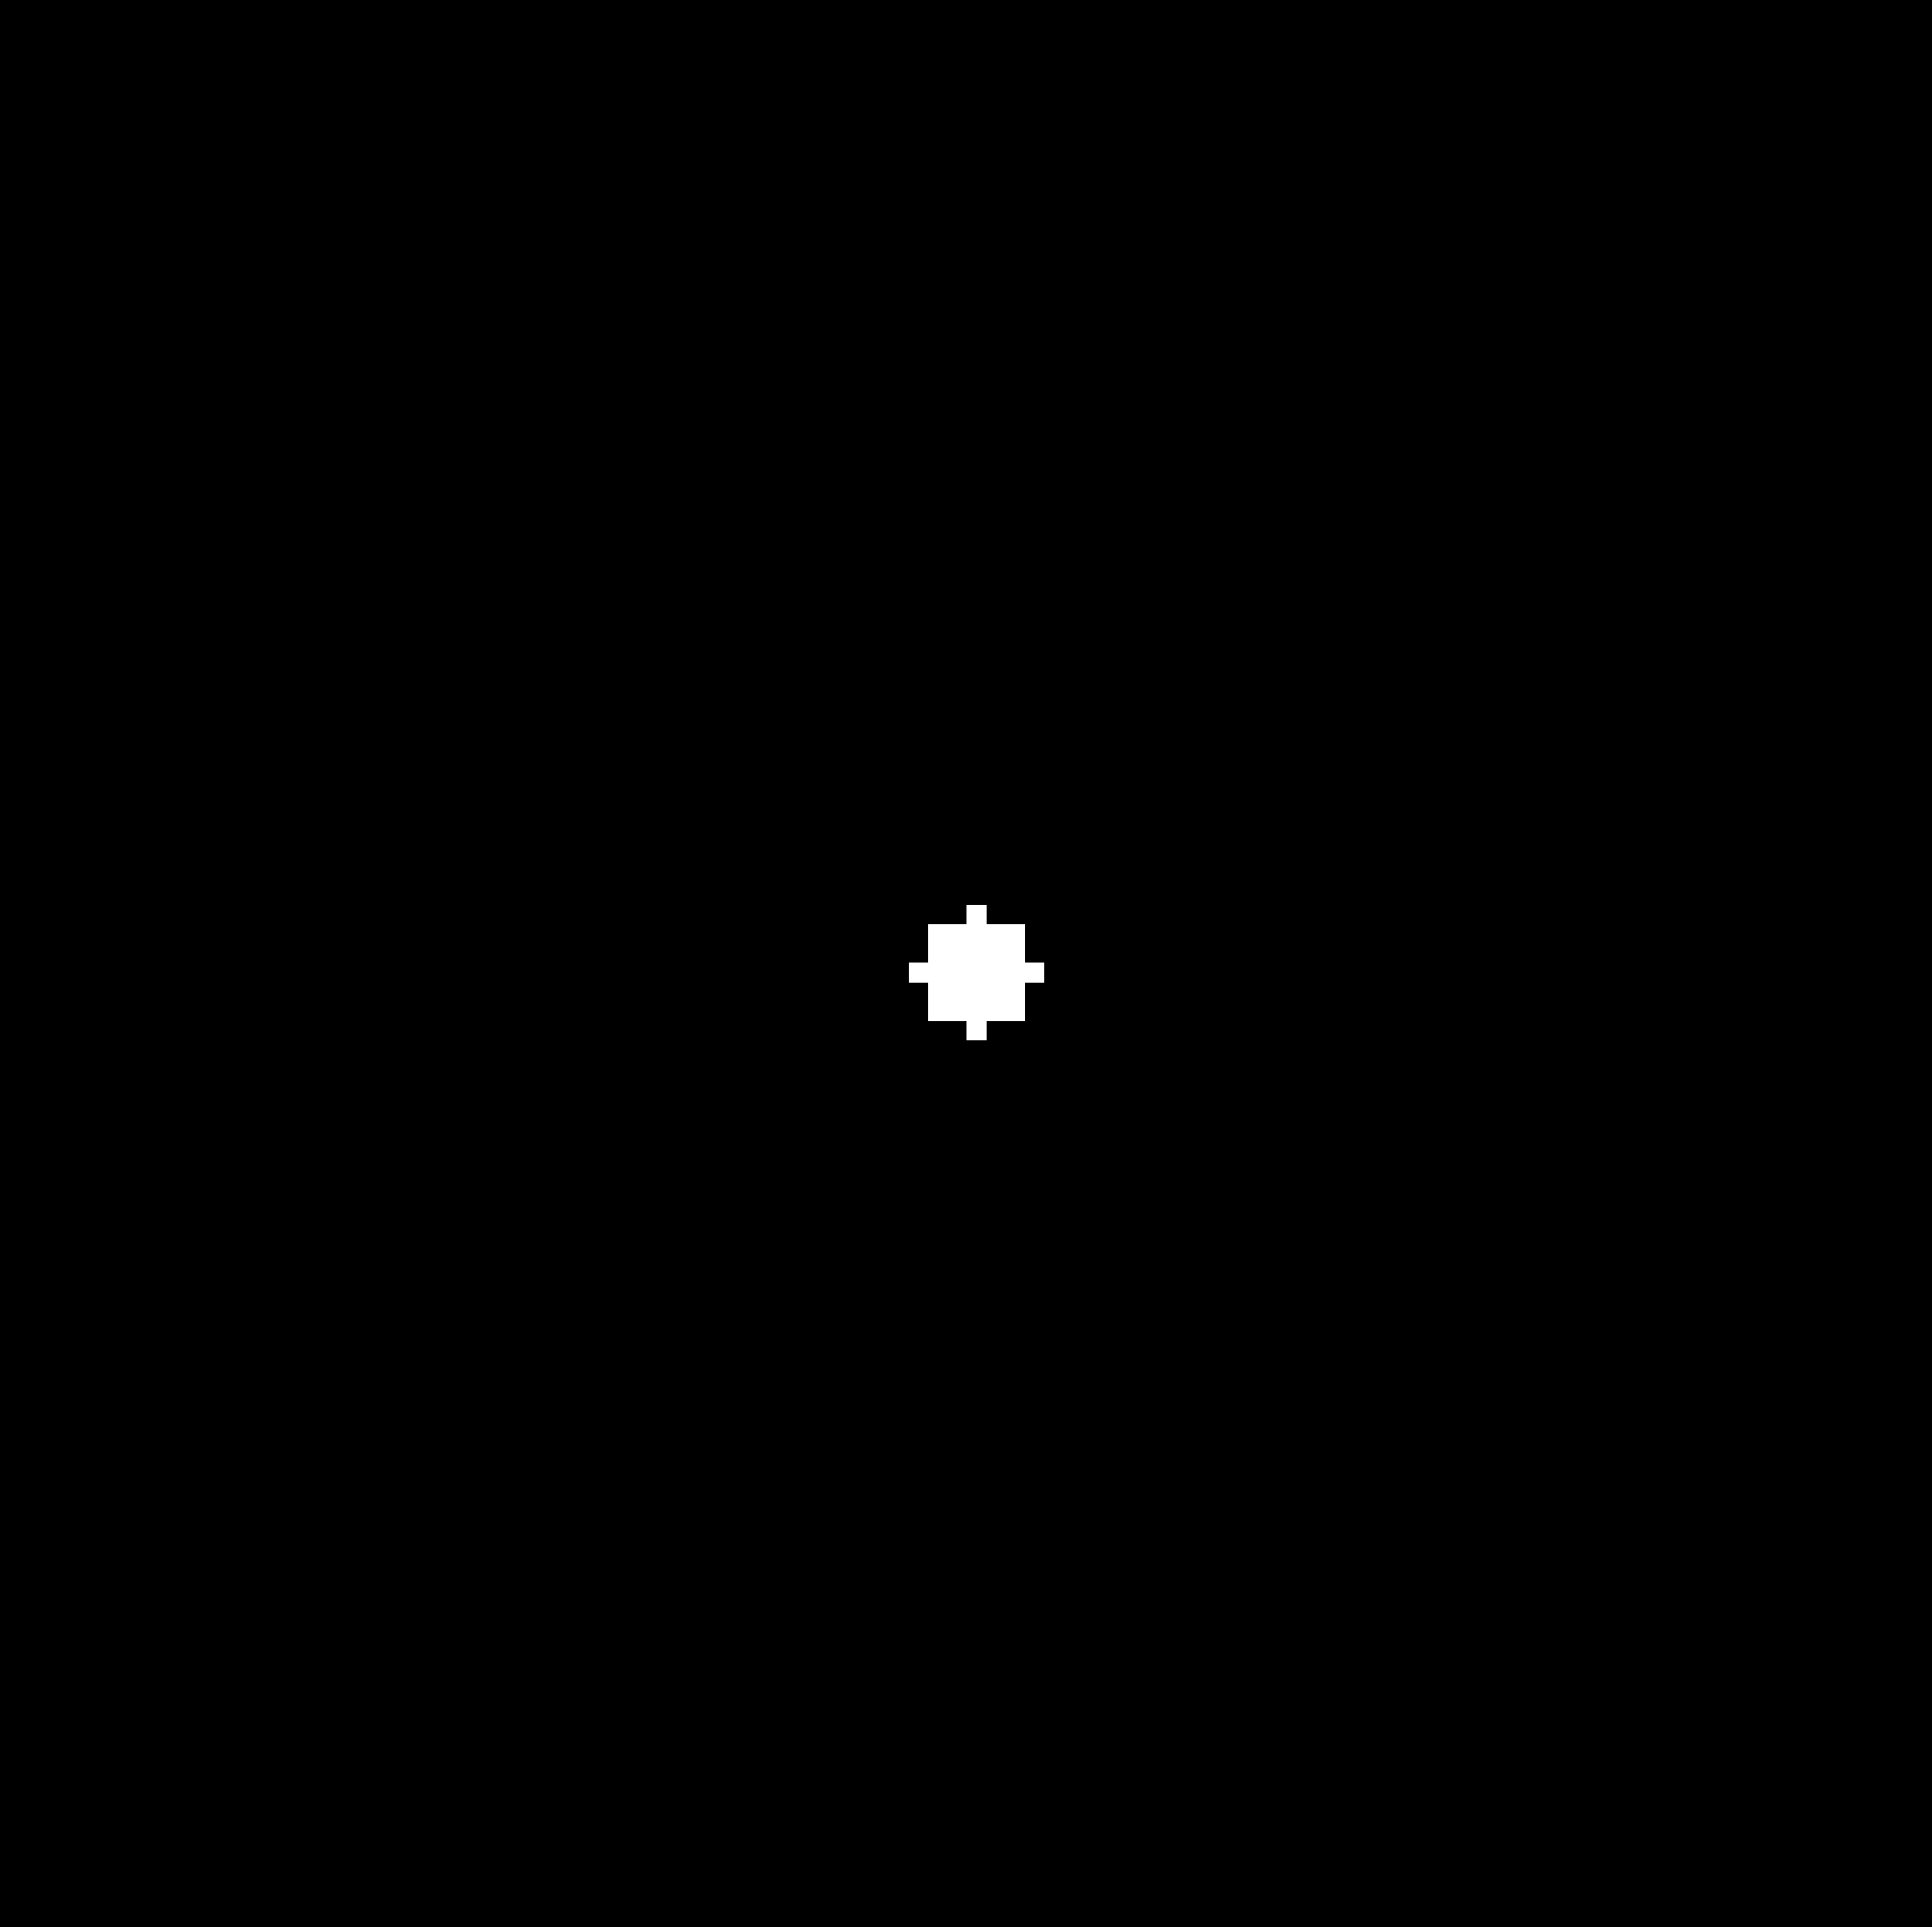
\includegraphics[width=0.3\textwidth]{Figuras/sinograma_circulo.png}
   \caption{(a) Imagen del círculo de 3 pixeles de radio. (b) Sinograma generado del círculo. }
   \label{fig:sinograma_circulo}
\end{figure}


\begin{figure}[H]
   \centering
       \begin{subfigure}[h]{0.24\textwidth}
           \centering
           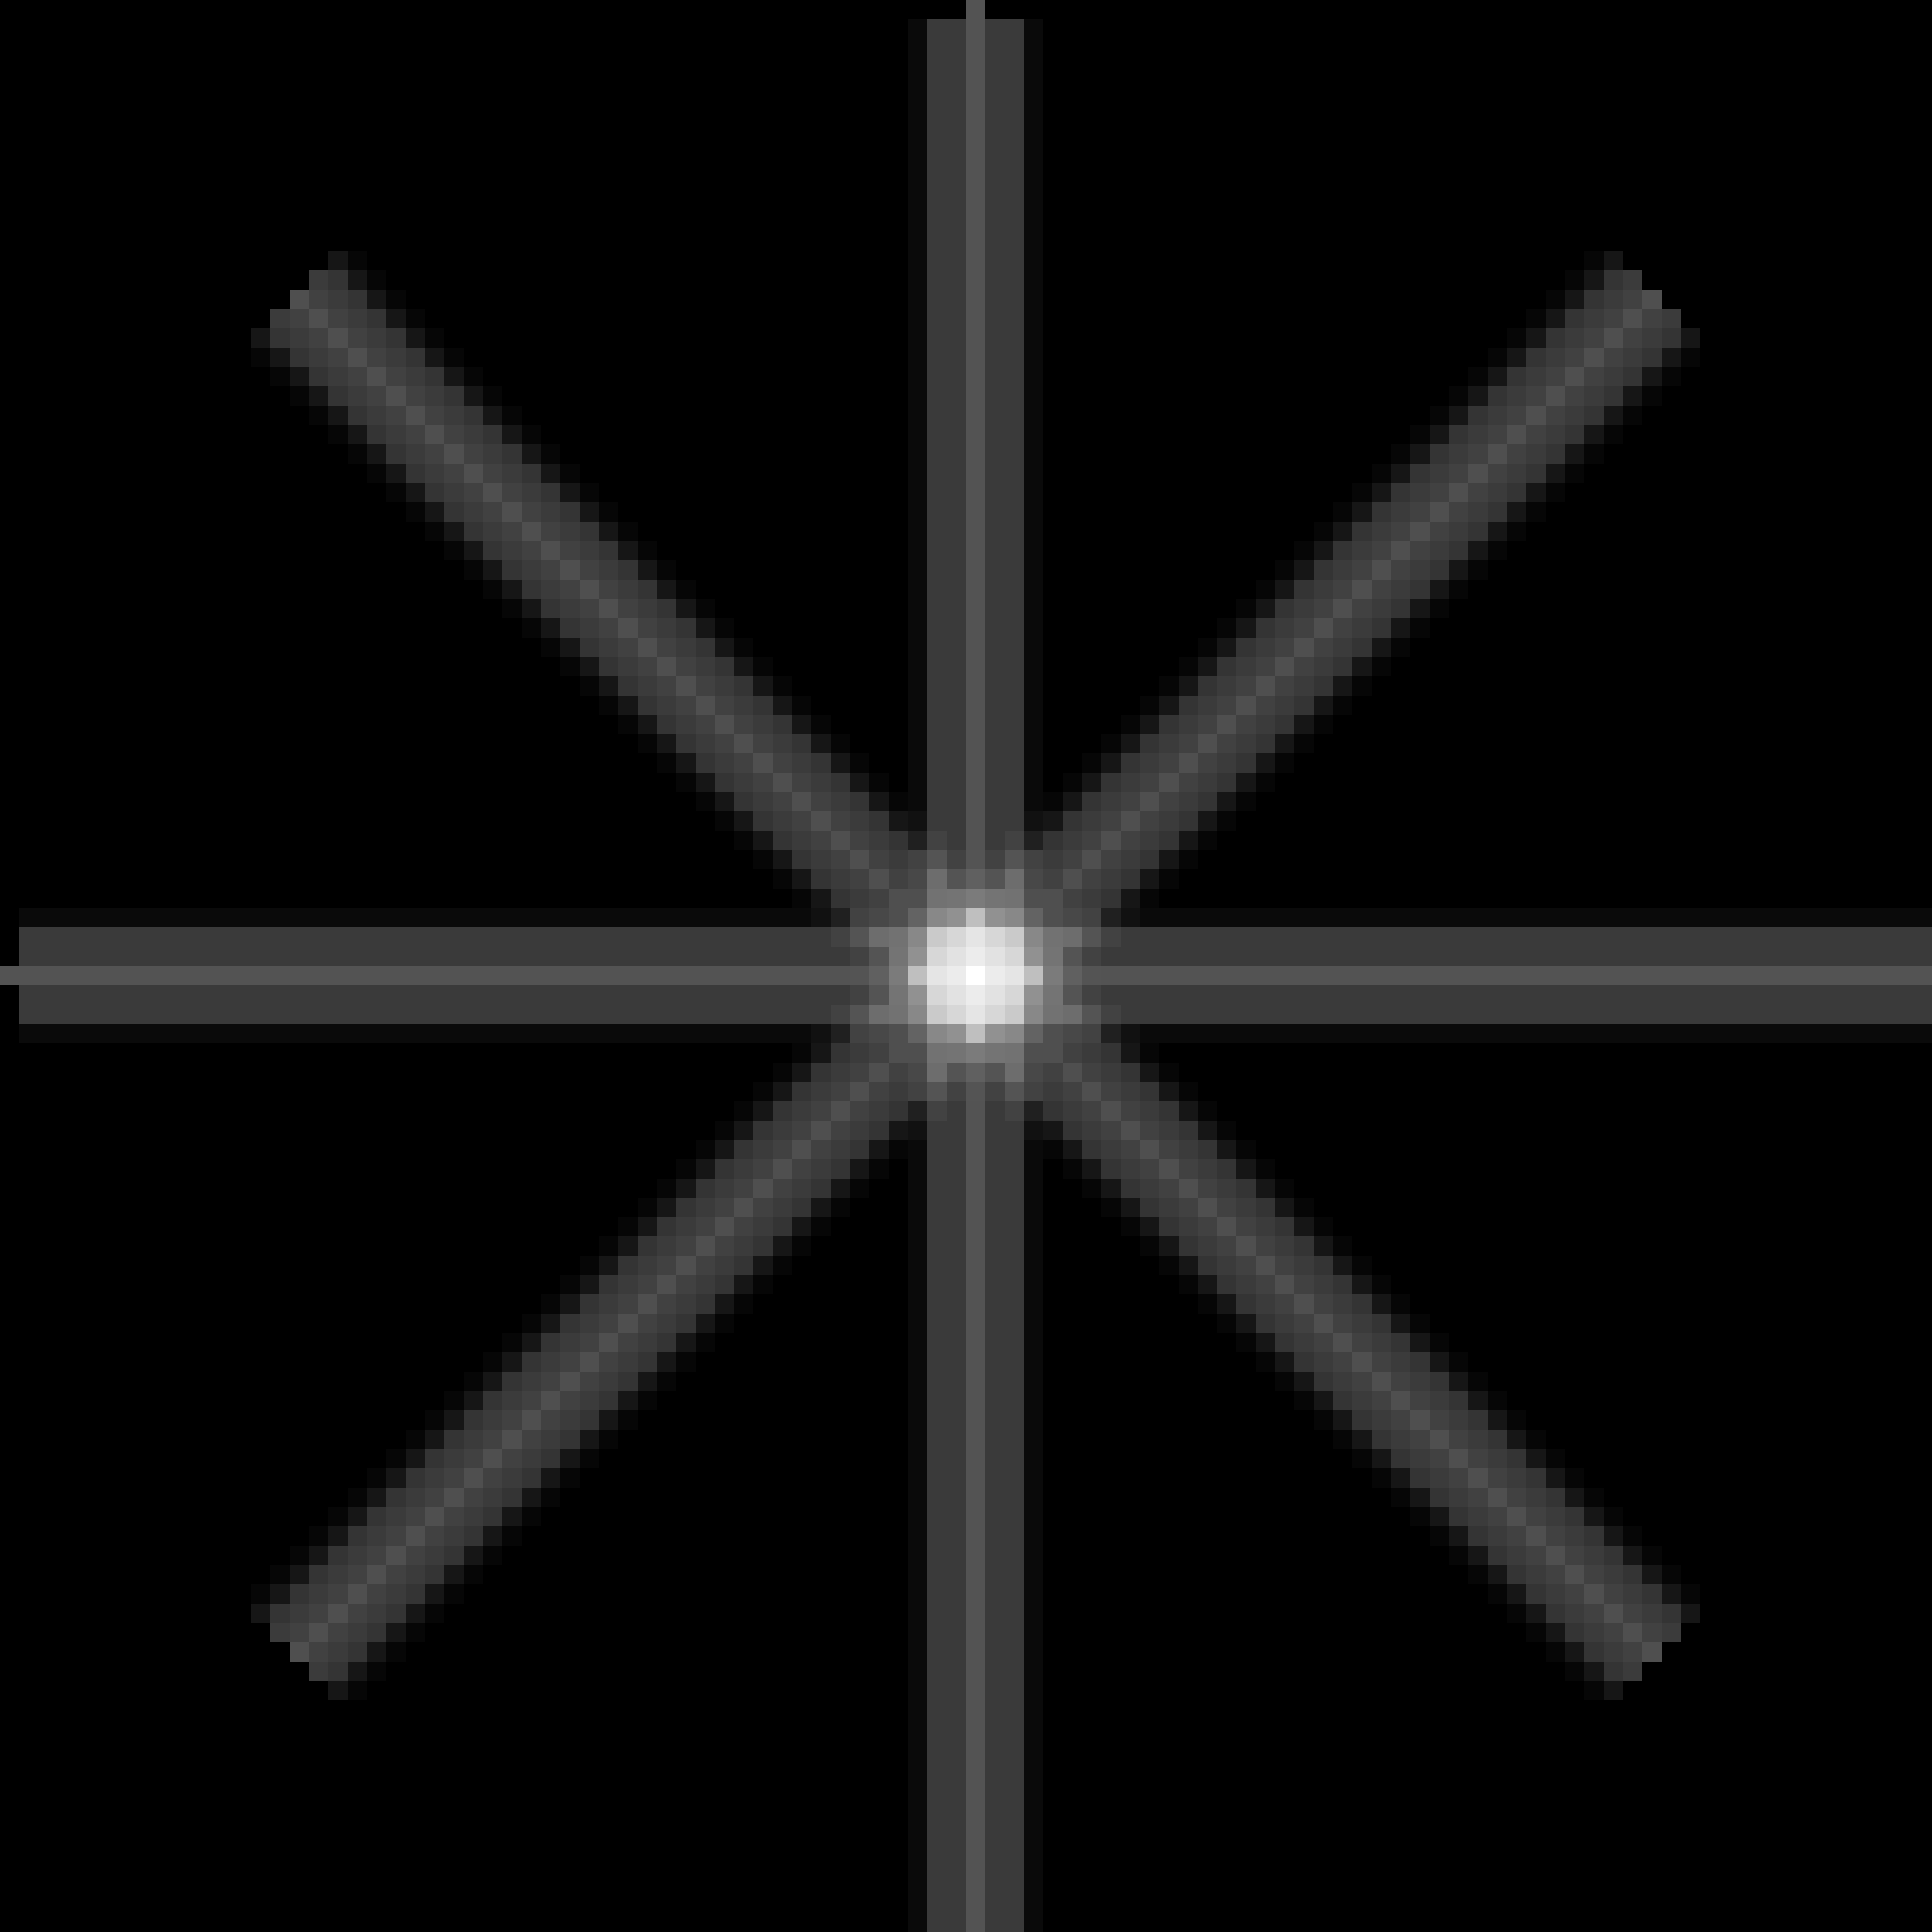
\includegraphics[width=\textwidth]{Figuras/retroproyeccion_p=8_filter=none.png} 
       \end{subfigure}
       \begin{subfigure}[h]{0.24\textwidth}
           \centering
           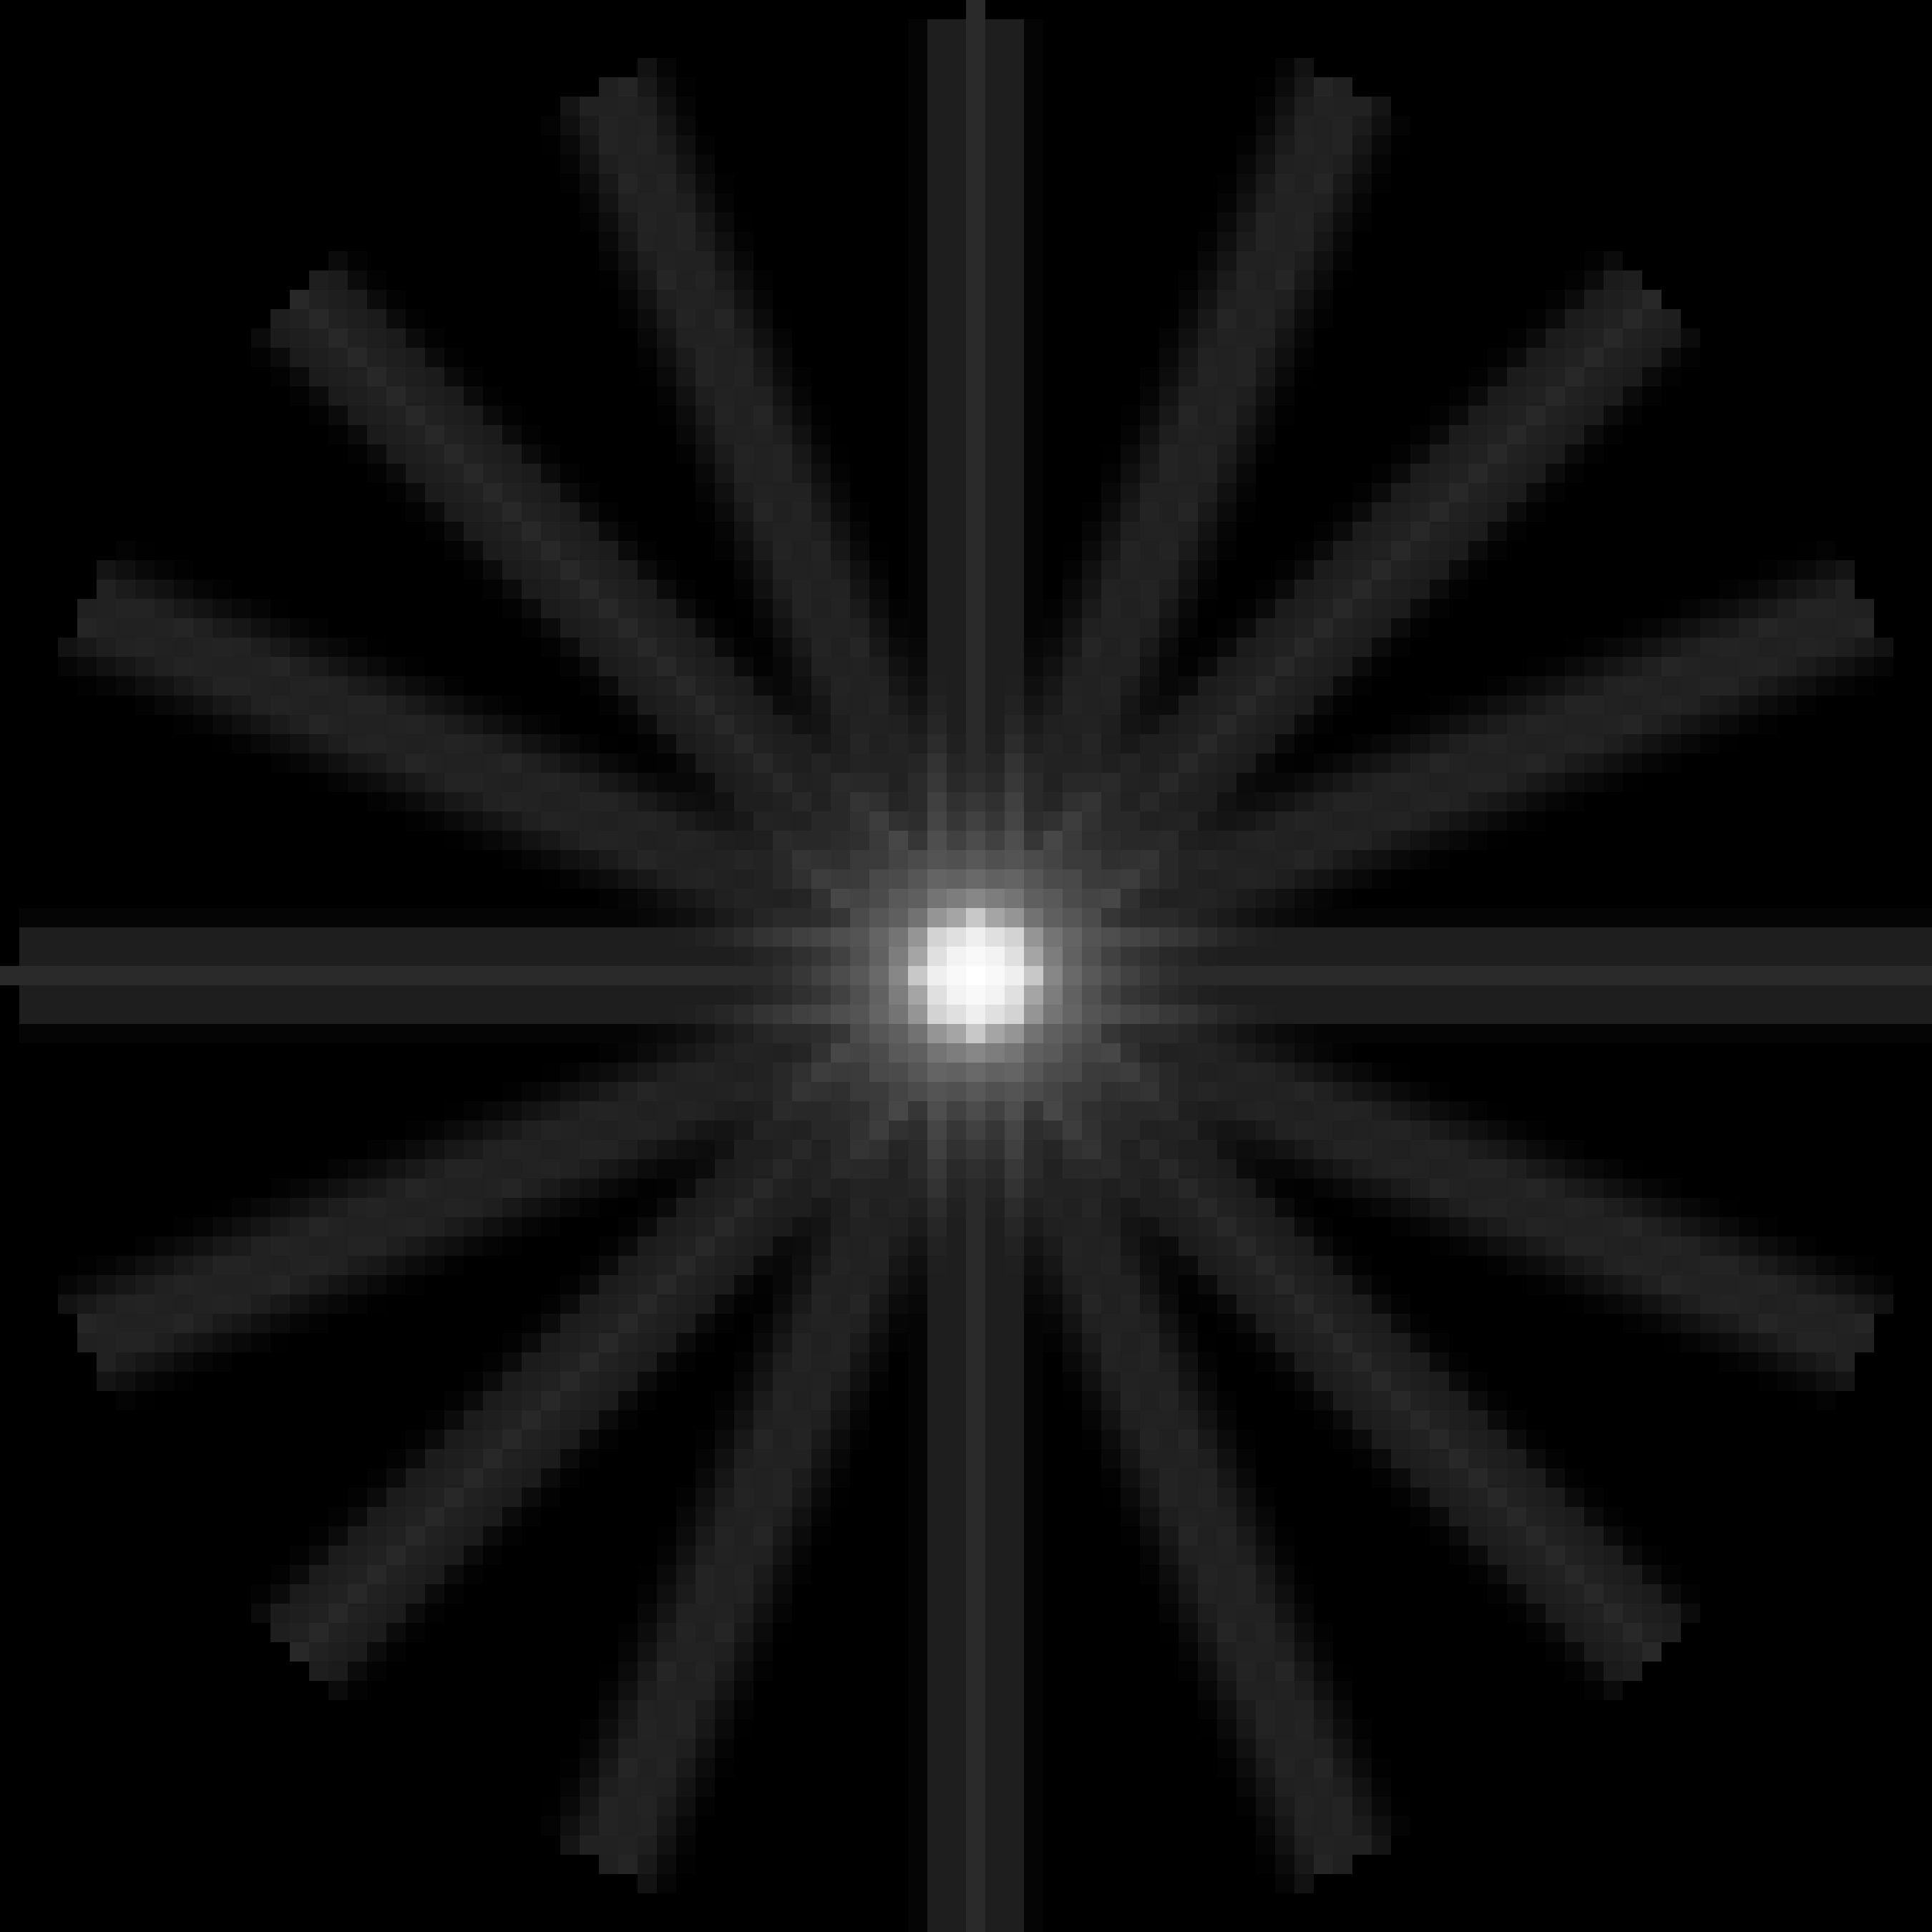
\includegraphics[width=\textwidth]{Figuras/retroproyeccion_p=16_filter=none.png}
       \end{subfigure}
       \begin{subfigure}[h]{0.24\textwidth}
           \centering
           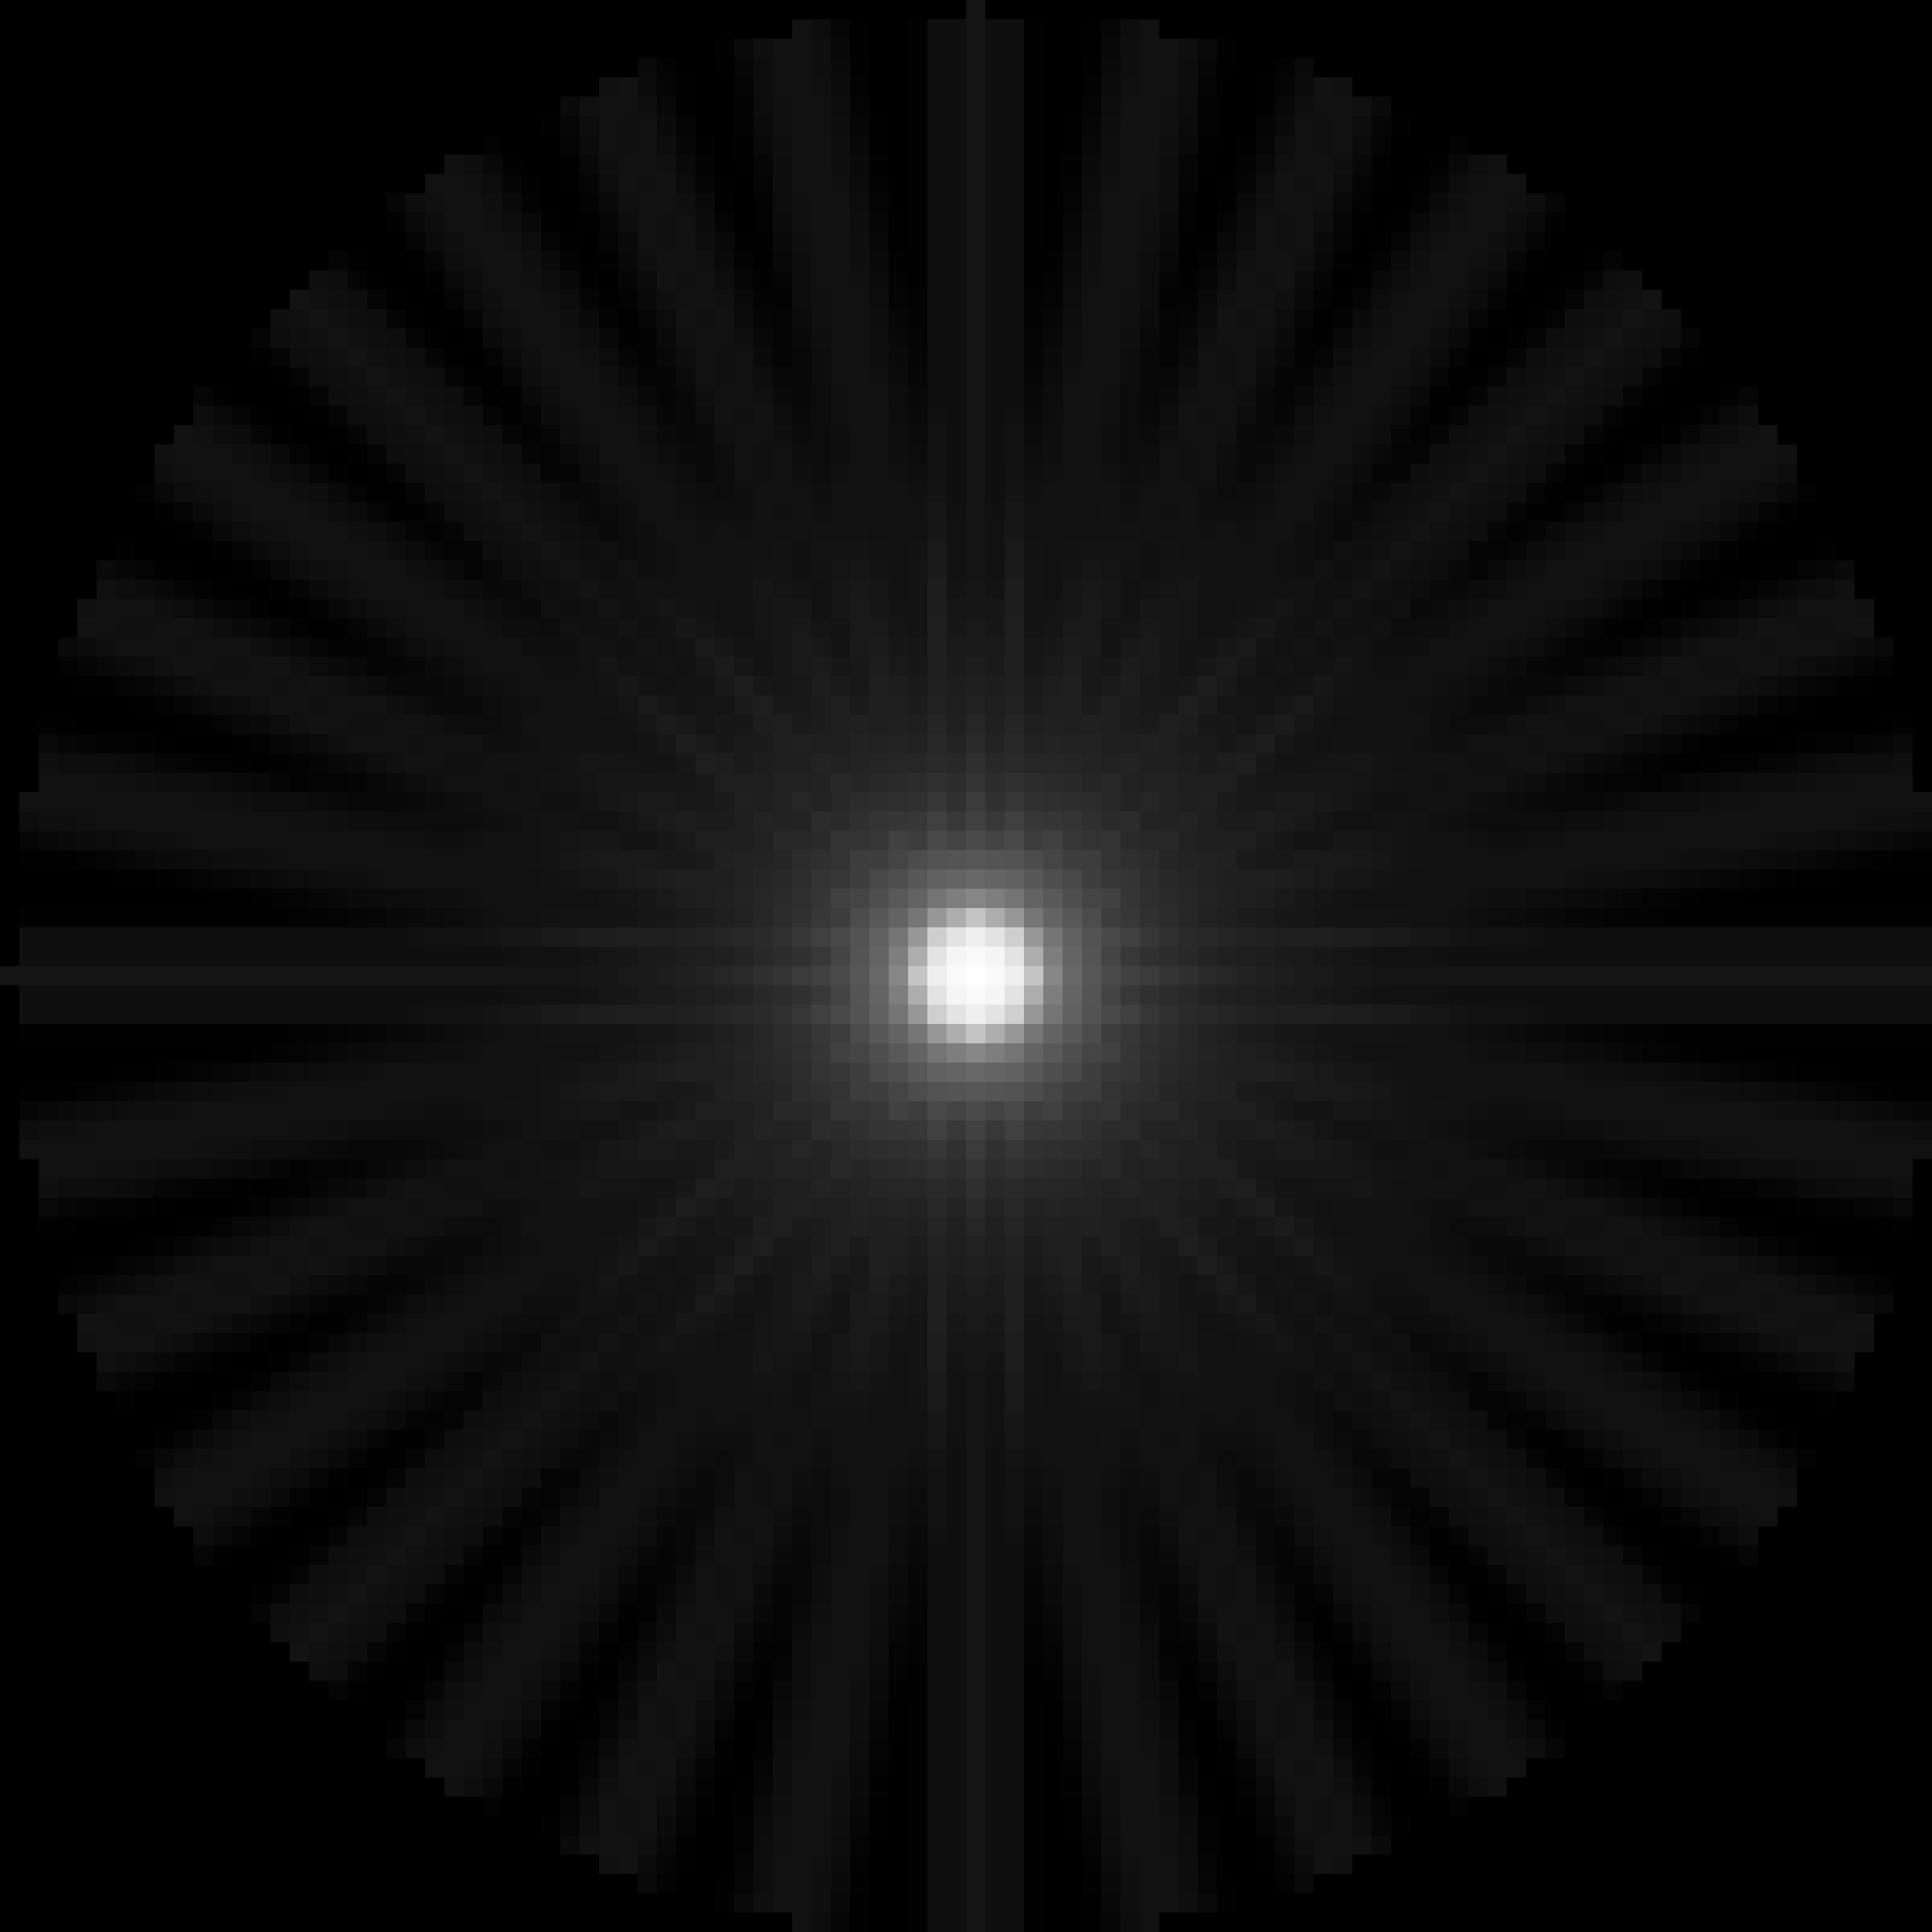
\includegraphics[width=\textwidth]{Figuras/retroproyeccion_p=32_filter=none.png}
       \end{subfigure}
       \begin{subfigure}[h]{0.24\textwidth}
           \centering
           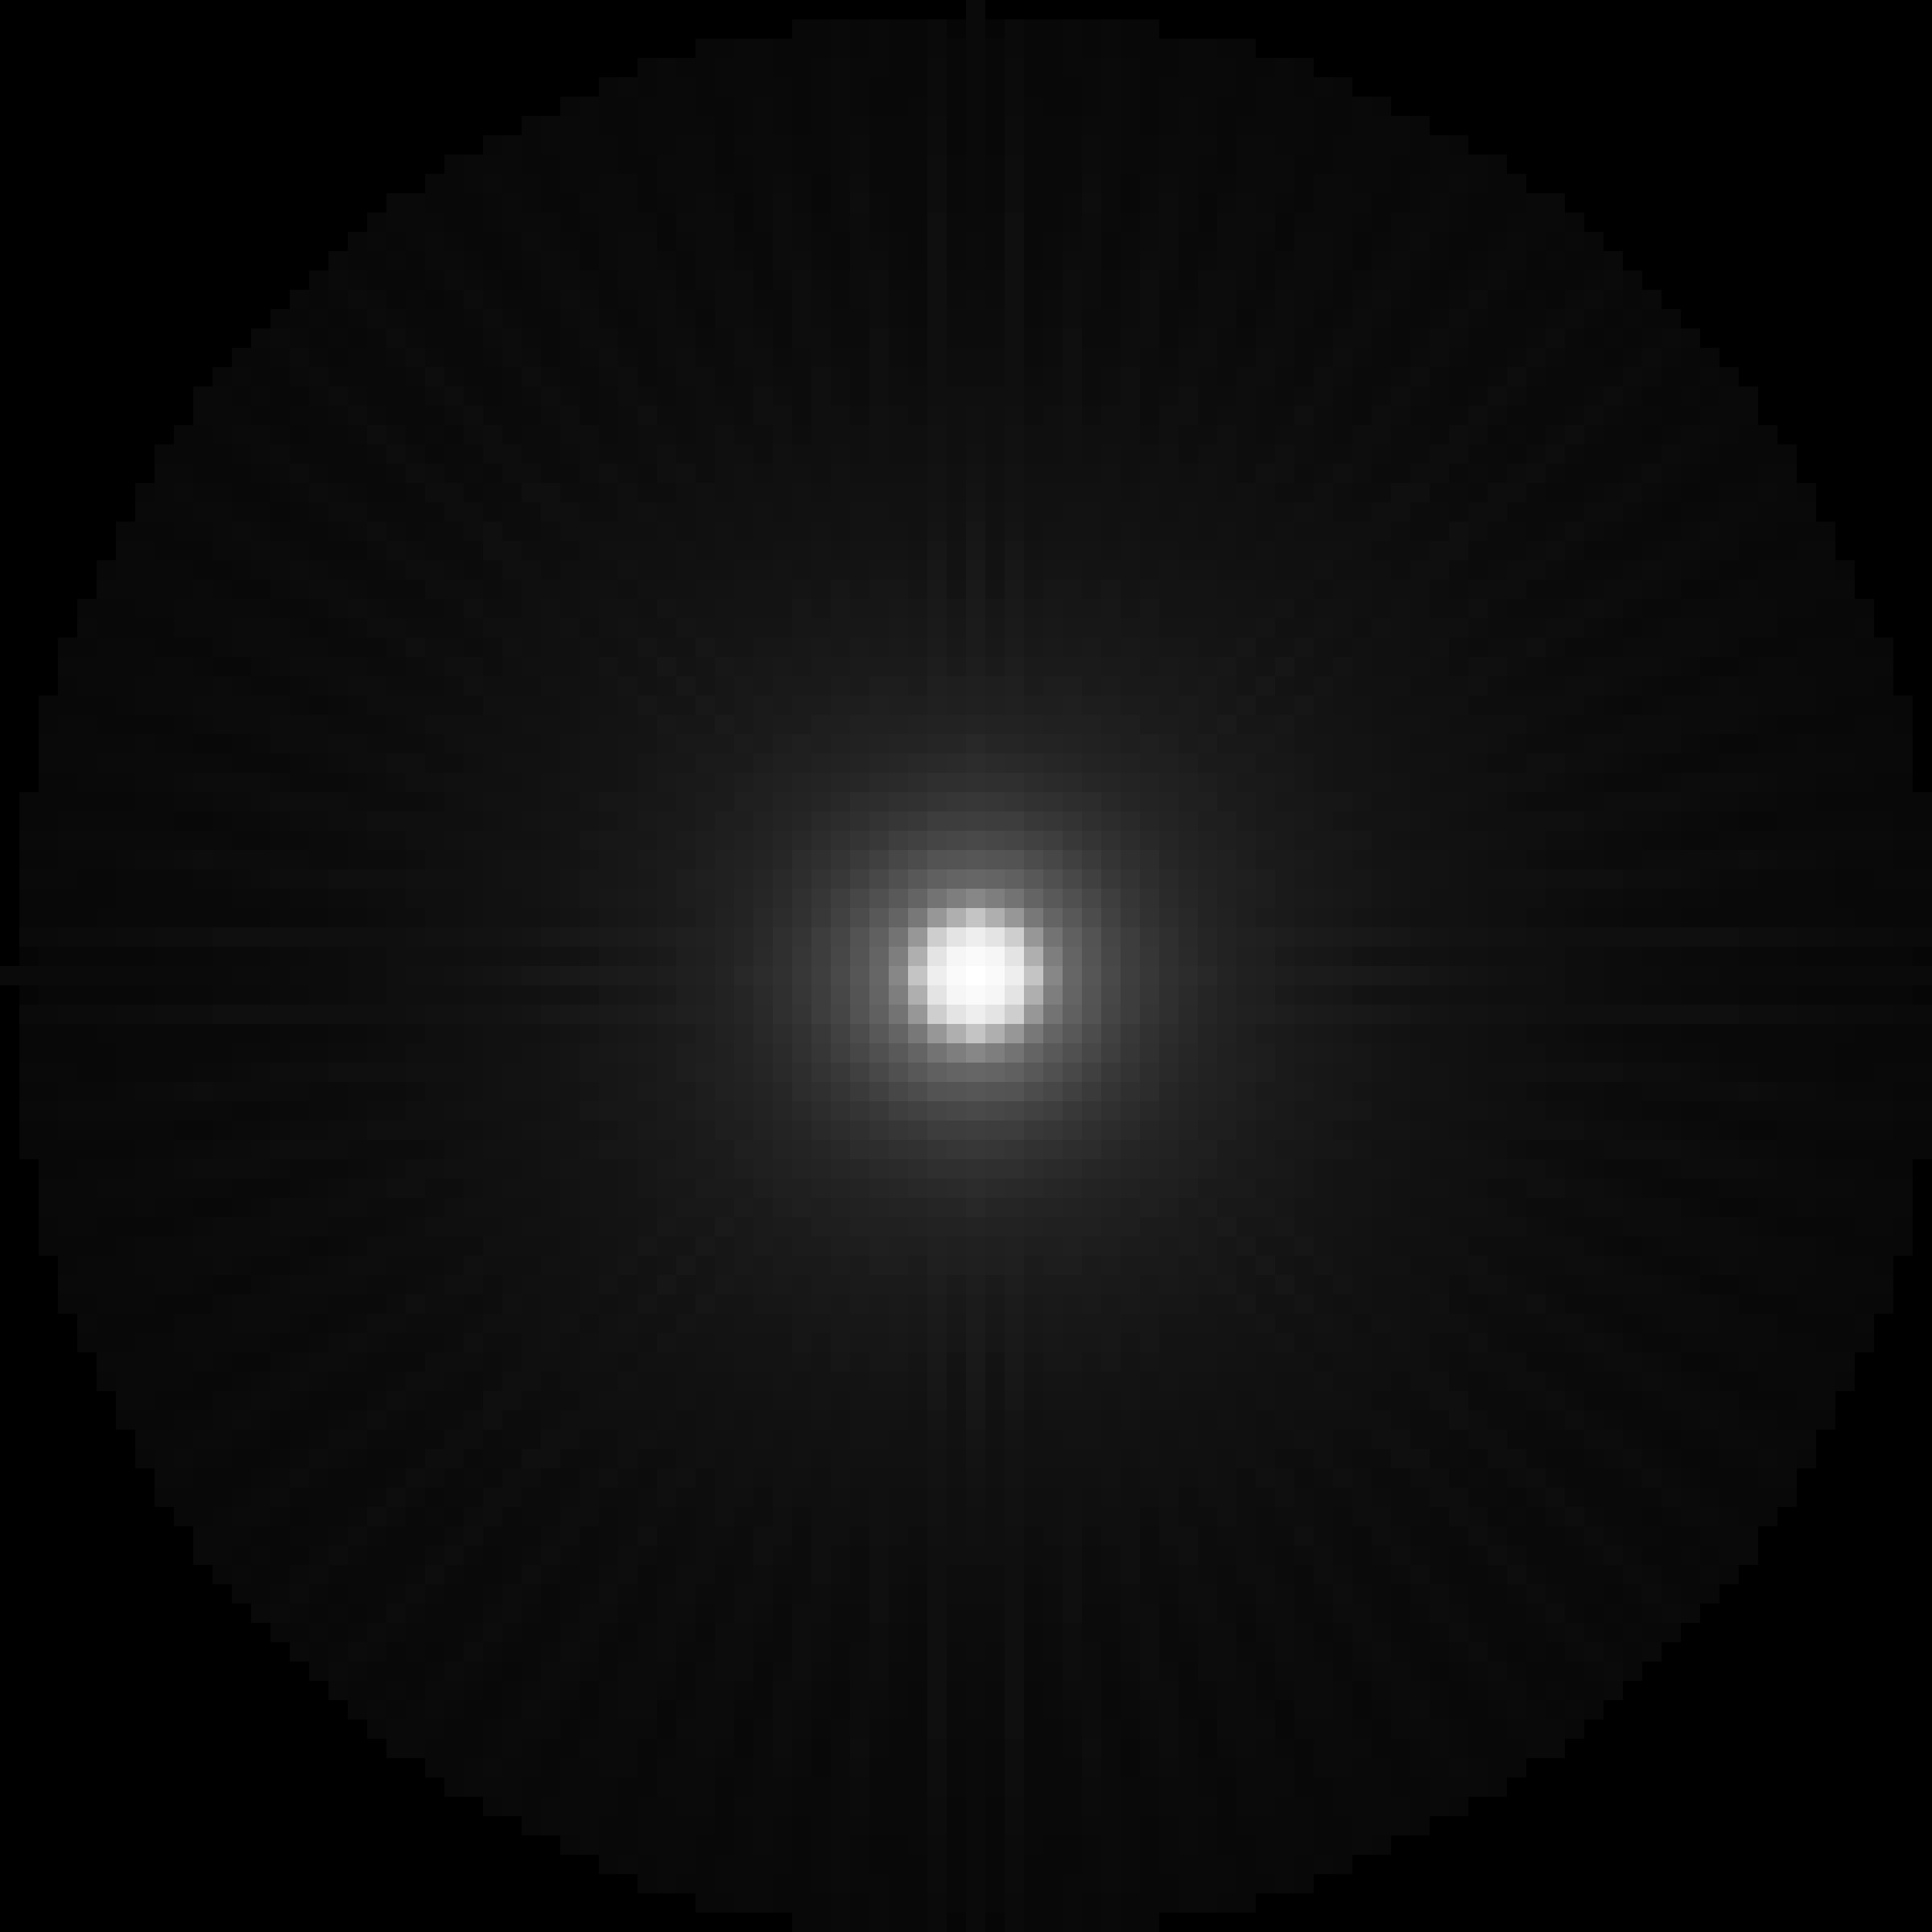
\includegraphics[width=\textwidth]{Figuras/retroproyeccion_p=64_filter=none.png}
       \end{subfigure}
        \begin{subfigure}[h]{0.24\textwidth}
           \centering
           
\includegraphics[width=\textwidth]{Figuras/retroproyeccion_p=8_filter=ramp.png}
           \caption{8 proyecciones.} 
        \end{subfigure}
        \begin{subfigure}[h]{0.24\textwidth}
           \centering
           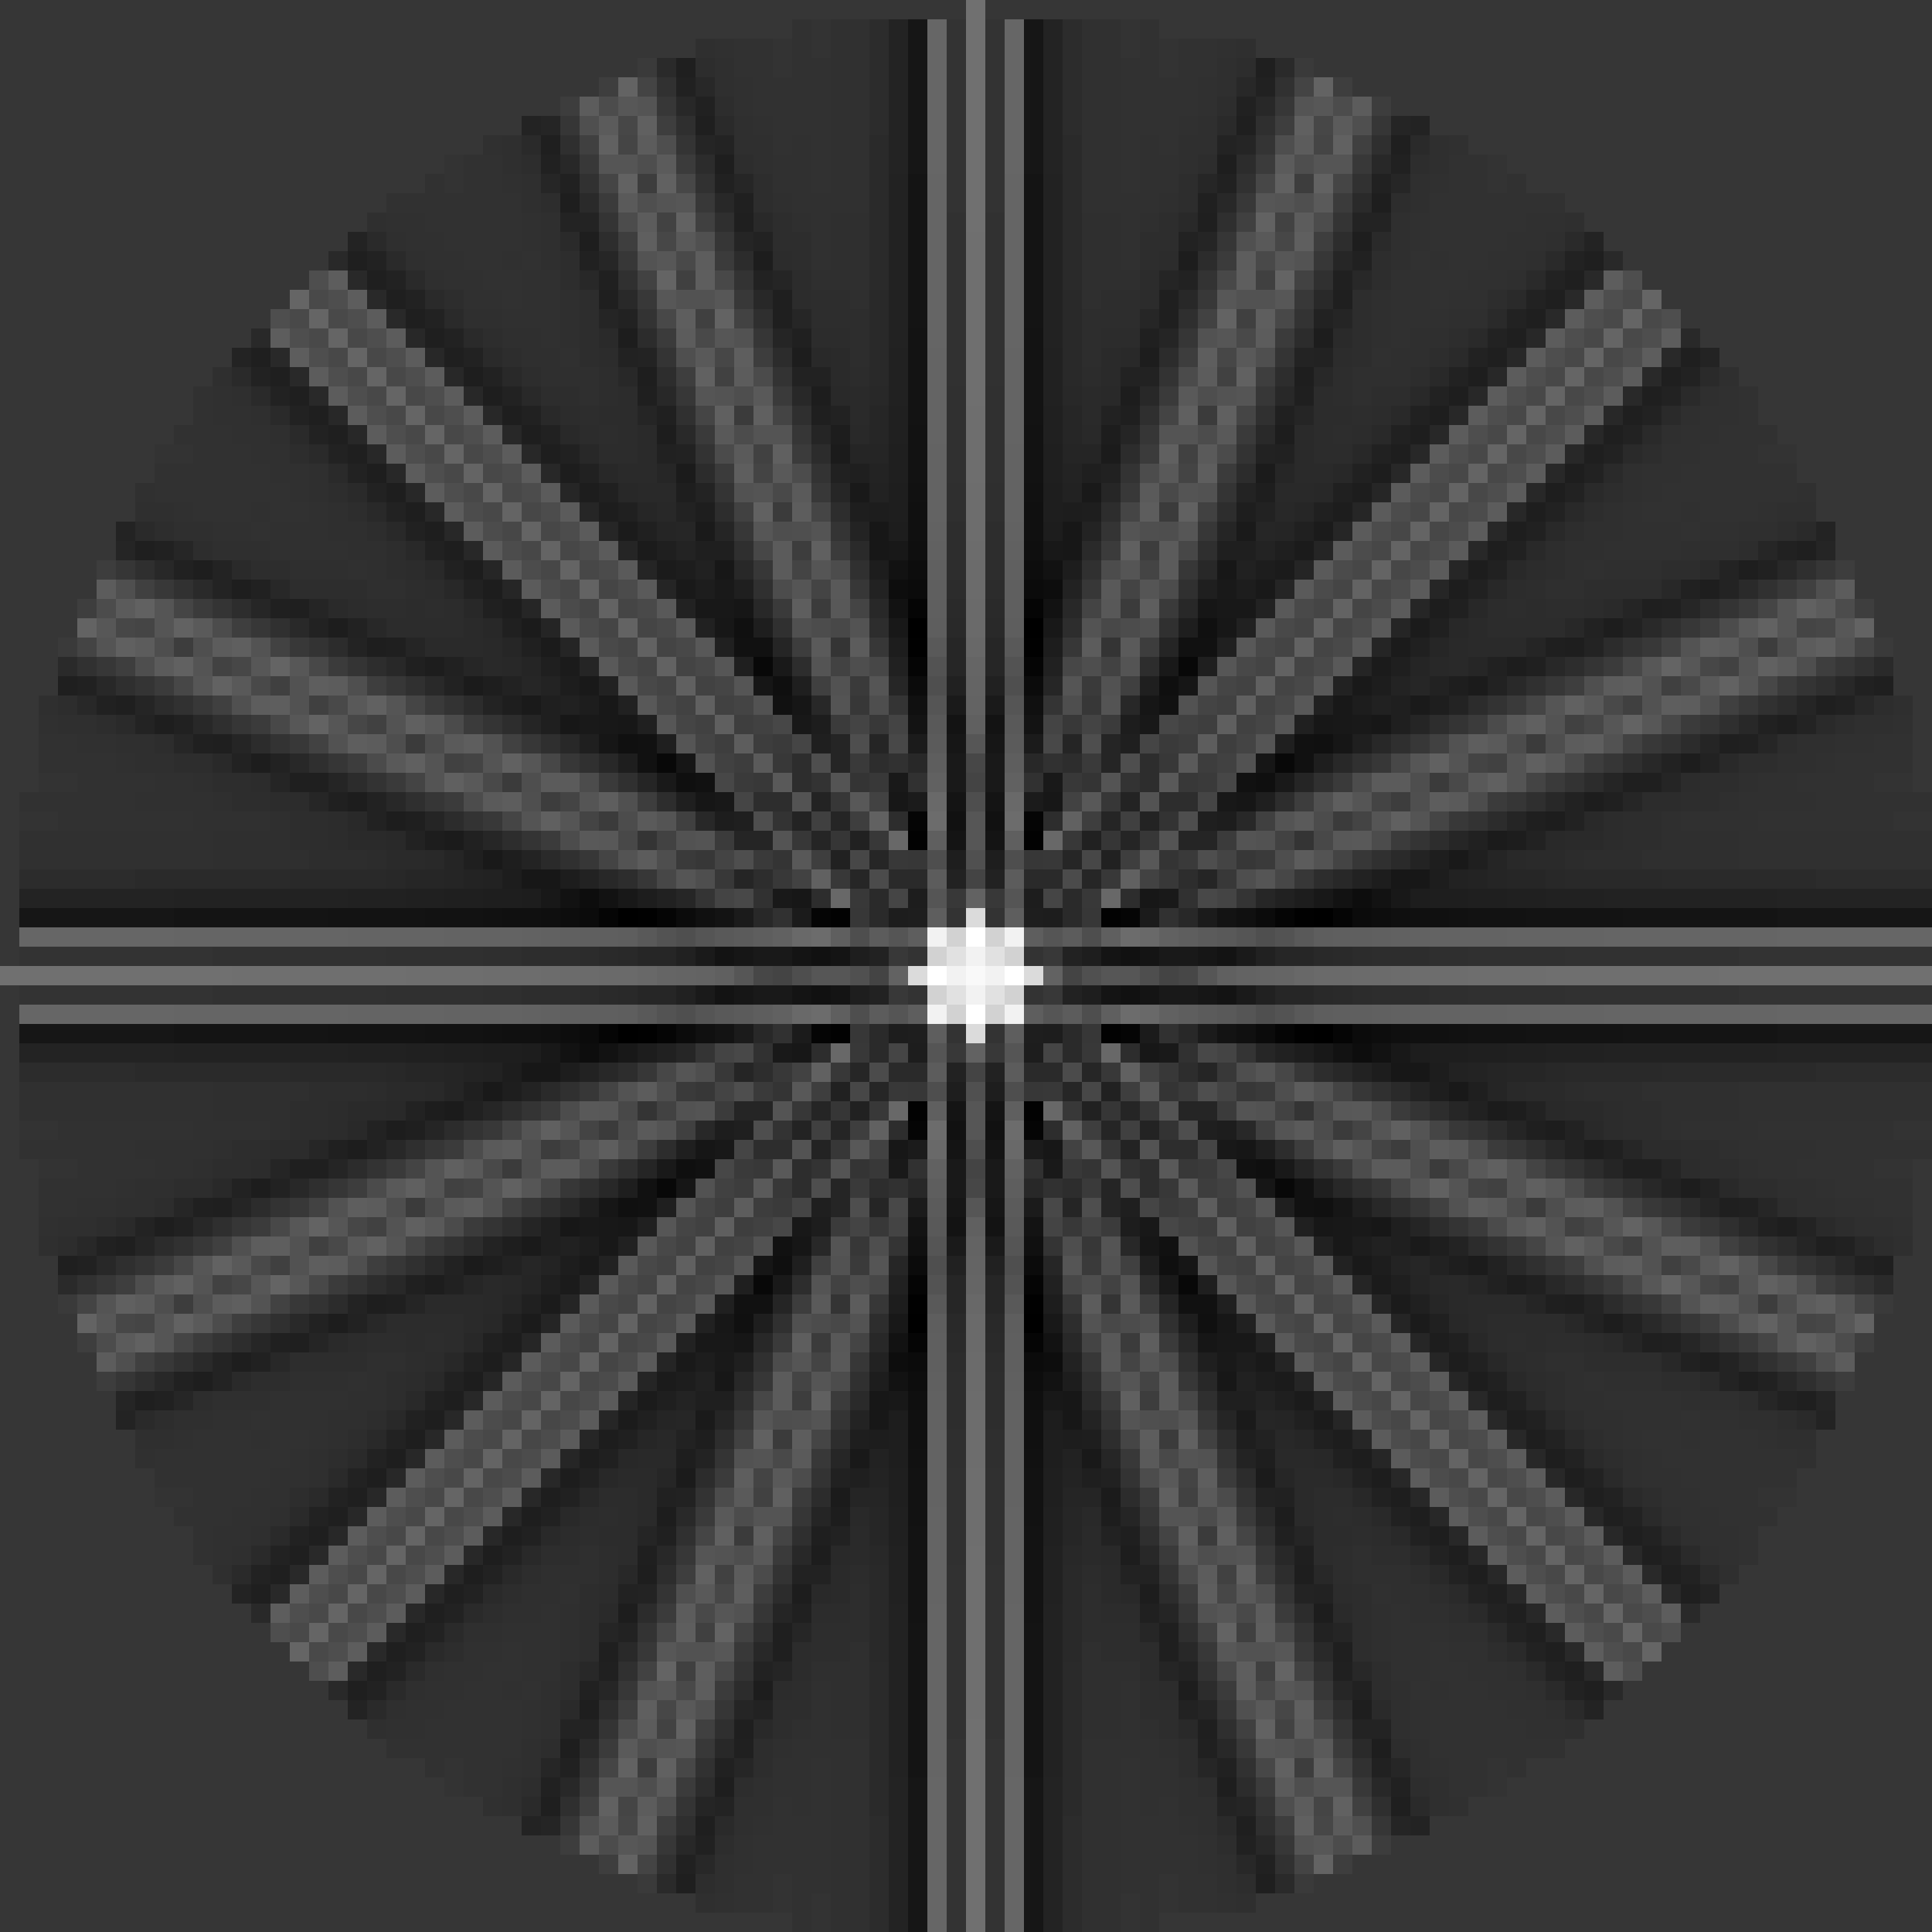
\includegraphics[width=\textwidth]{Figuras/retroproyeccion_p=16_filter=ramp.png}
           \caption{16 proyecciones.} 
        \end{subfigure}
        \begin{subfigure}[h]{0.24\textwidth}
           \centering
           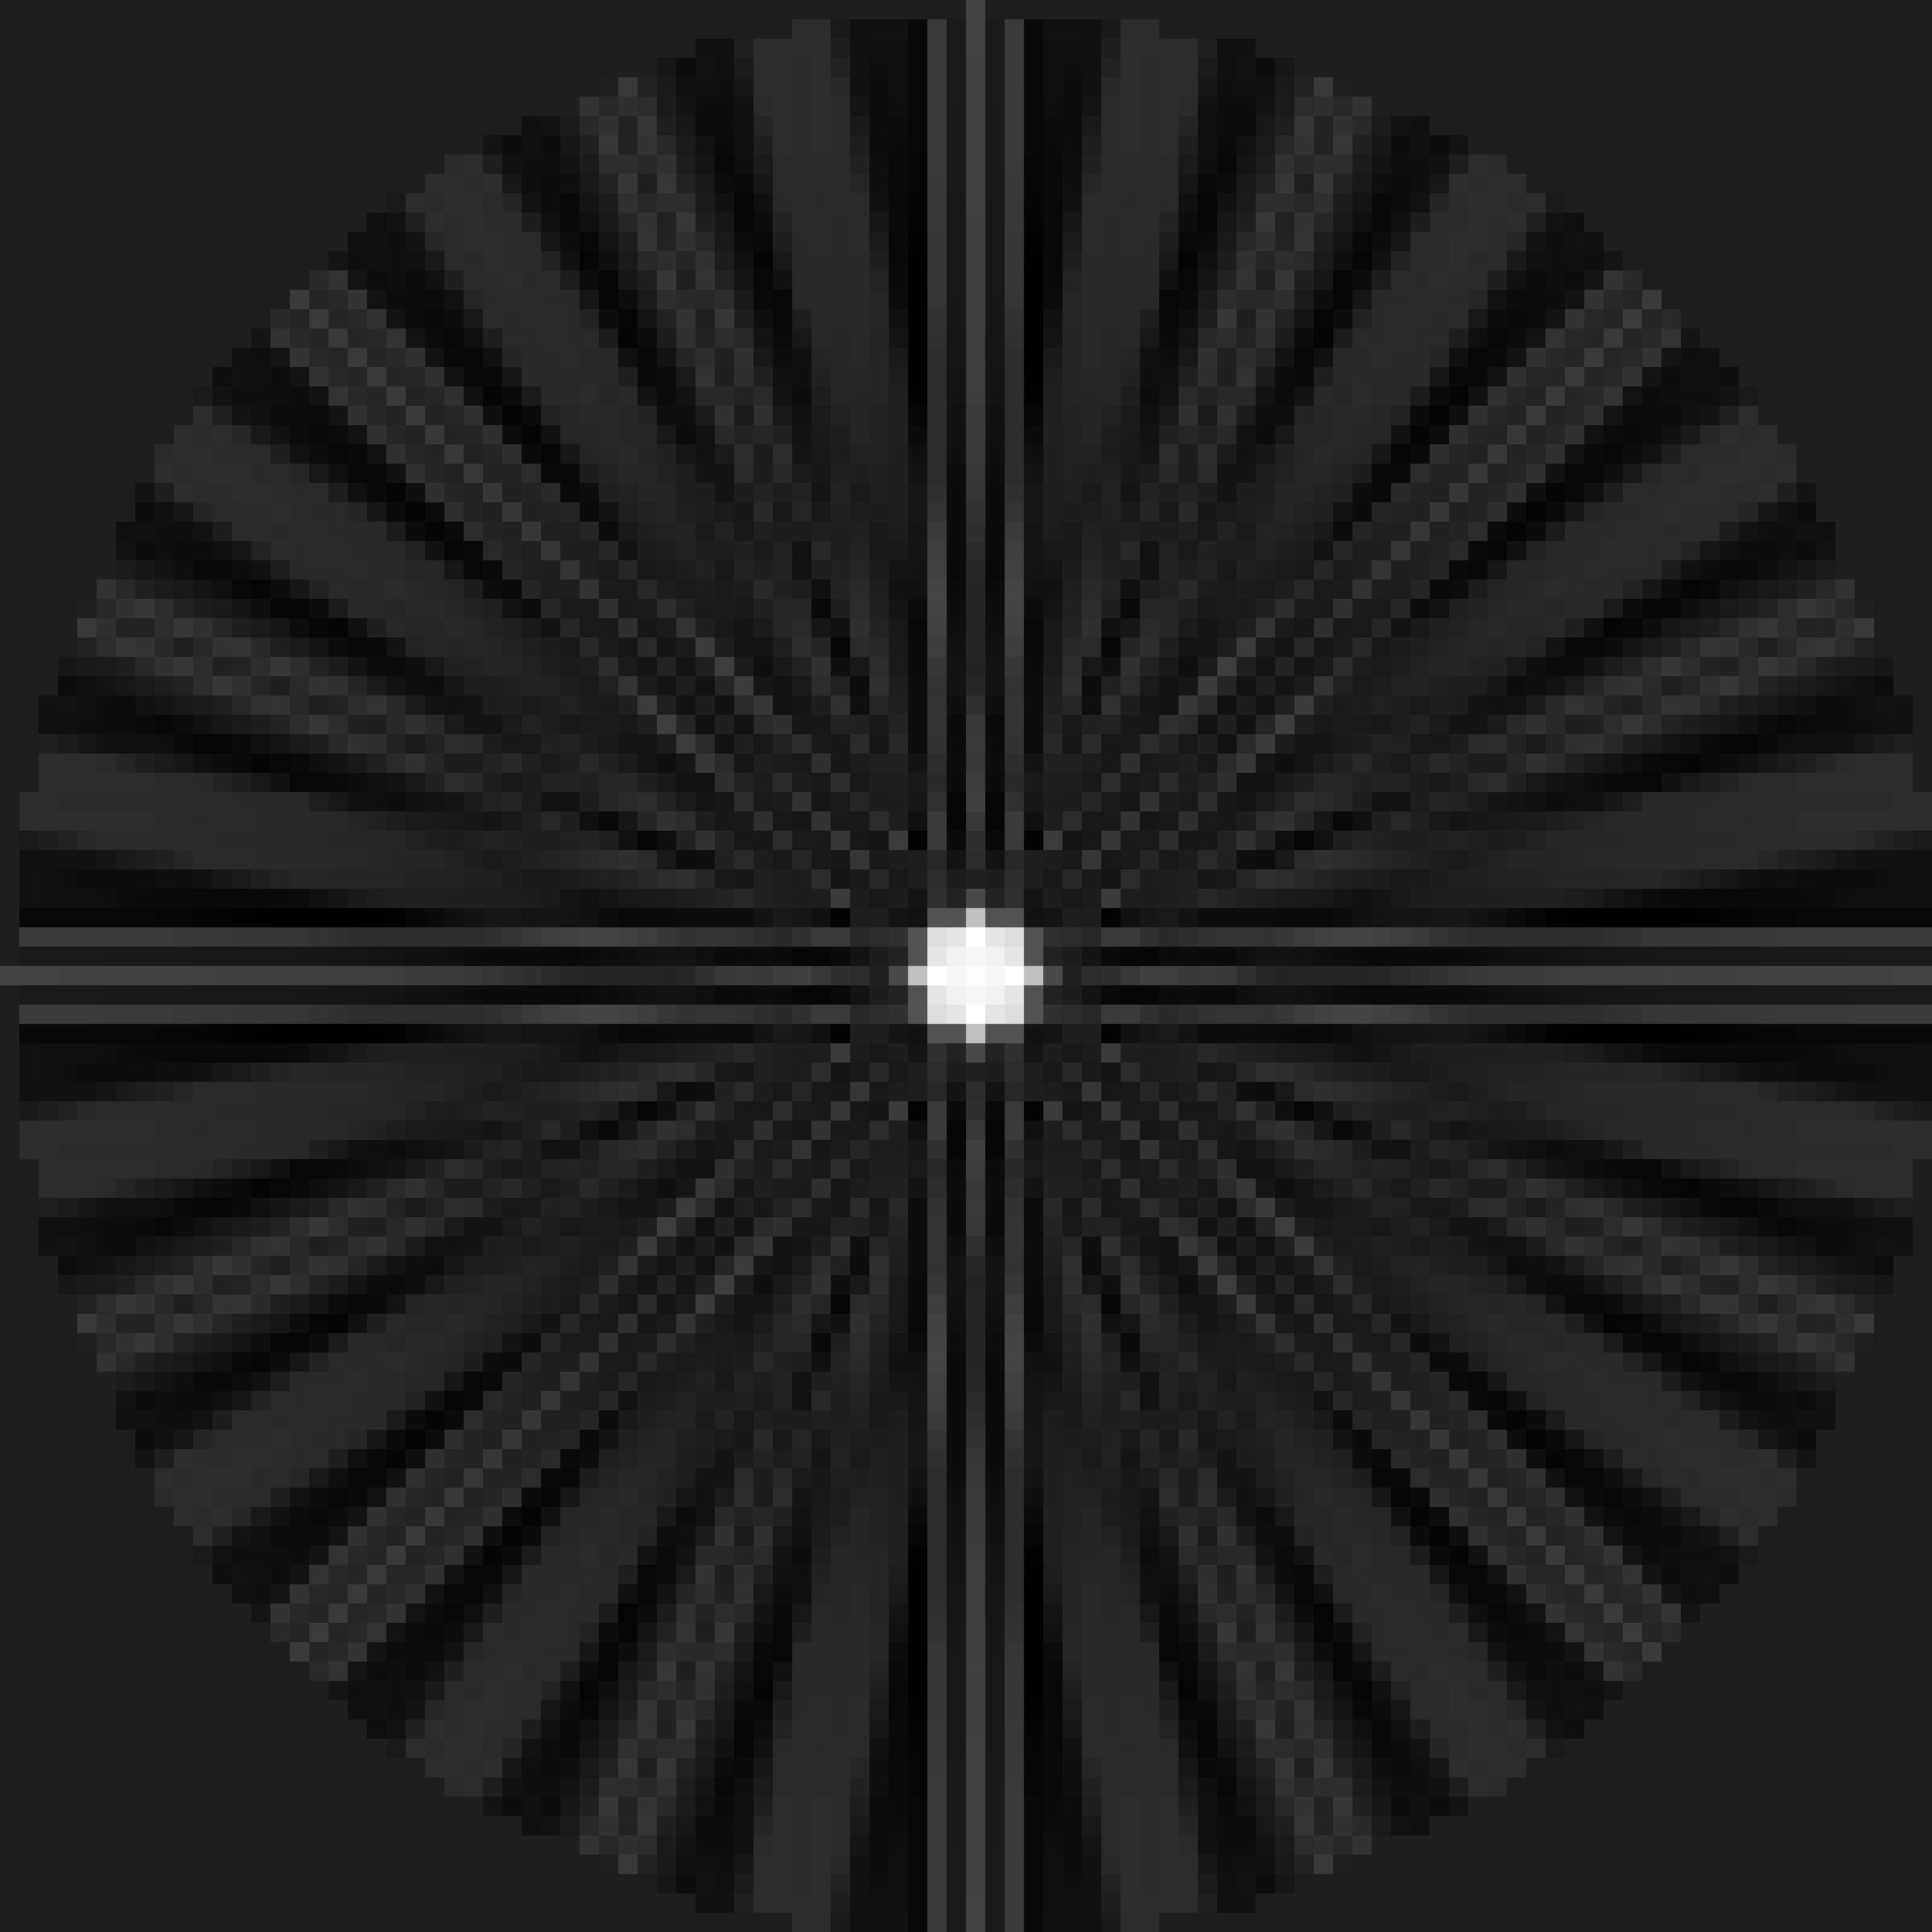
\includegraphics[width=\textwidth]{Figuras/retroproyeccion_p=32_filter=ramp.png}
           \caption{32 proyecciones.} 
        \end{subfigure}
        \begin{subfigure}[h]{0.24\textwidth}
           \centering
           
\includegraphics[width=\textwidth]{Figuras/retroproyeccion_p=64_filter=ramp.png}
           \caption{64 proyecciones.} 
        \end{subfigure}
   \caption{Retroproyeccion del círculo (Fig. \ref{fig:sinograma_circulo}) para 100 detectores y $8,16,32,64$ proyecciones. Arriba: Retroproyección sin filtro. Abajo: Retroproyección con filtro rampa.}
   \label{fig:retroproyeccion_circulo}
\end{figure}

Sin filtro se ve el halo de la retroproyección, que se reduce al aplicar el filtro rampa. Además, se observa que a medida que se aumenta el número de proyecciones, la retroproyección se asemeja más al círculo original.


\section{Defecto de un detector}

En esta sección se estudiará que sucede cuando un detector no registra ninguna actividad. En primer lugar, este defecto se traduce en el sinograma como una columna oscura ya que en el eje horizontal se grafican el numero de detectores. En la parte superior de la Fig. \ref{fig:detector_roto} se muestran los sinogramas generados con 367 detectores y 320 proyecciones recorriendo media circunferencia con defectos en los detectores 50, 150, 250 y 300. En la parte inferior de la Fig. \ref{fig:detector_roto} se muestran las retroproyecciones filtradas con filtro rampa de los sinogramas con defectos. Se observa que, en todos los casos se obtiene un artefacto semicircular con 2 lineas tangentes a los extremos del semicirculo a la misma distancia del centro a la columna sin señal en el sinograma, además de otras distorsiones en la imagen. Notar que en el caso \ref{fig:sinograma_50}, la columna se encuentra parcialmente dentro del sinograma. En este caso, las lineas tangentes no son verticales como sucede en los otros tres casos donde los defectos están totalmente contenidos en la imagen. 

\begin{figure}[H]
   \centering
       \begin{subfigure}[h]{0.24\textwidth}
           \centering
           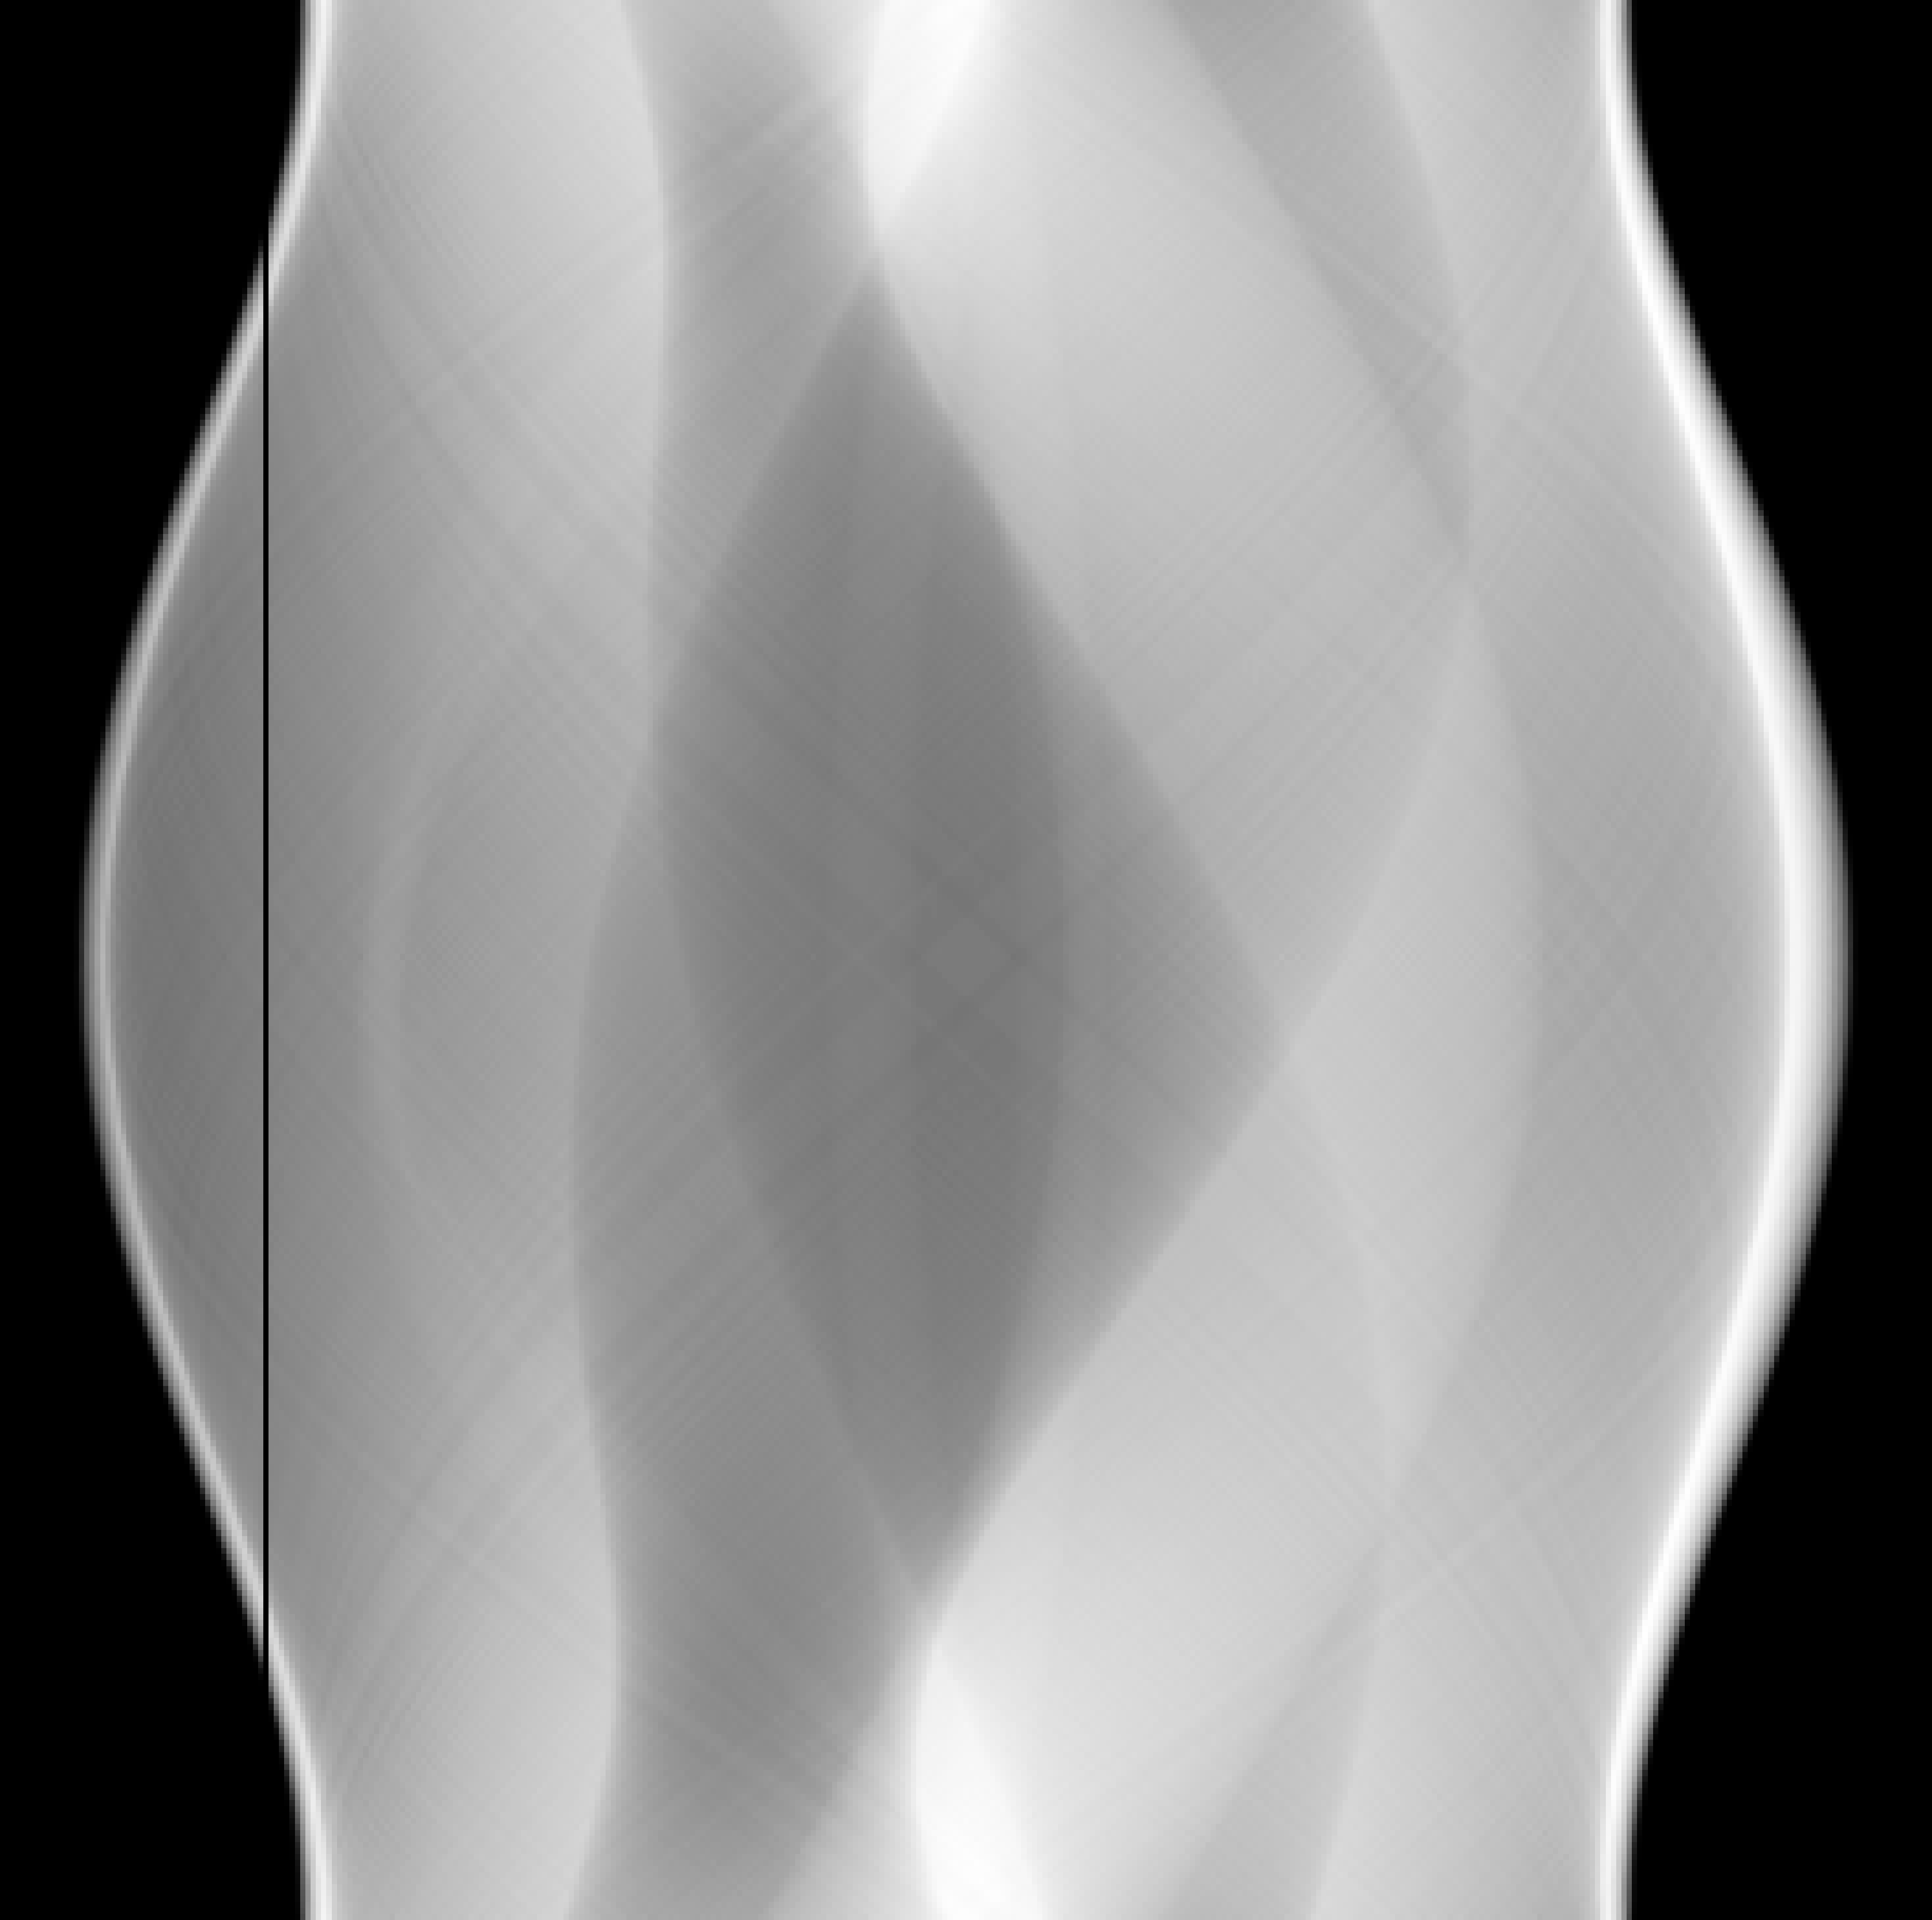
\includegraphics[width=\textwidth]{Figuras/sinograma_50.png} 
       \end{subfigure}
       \begin{subfigure}[h]{0.24\textwidth}
           \centering
           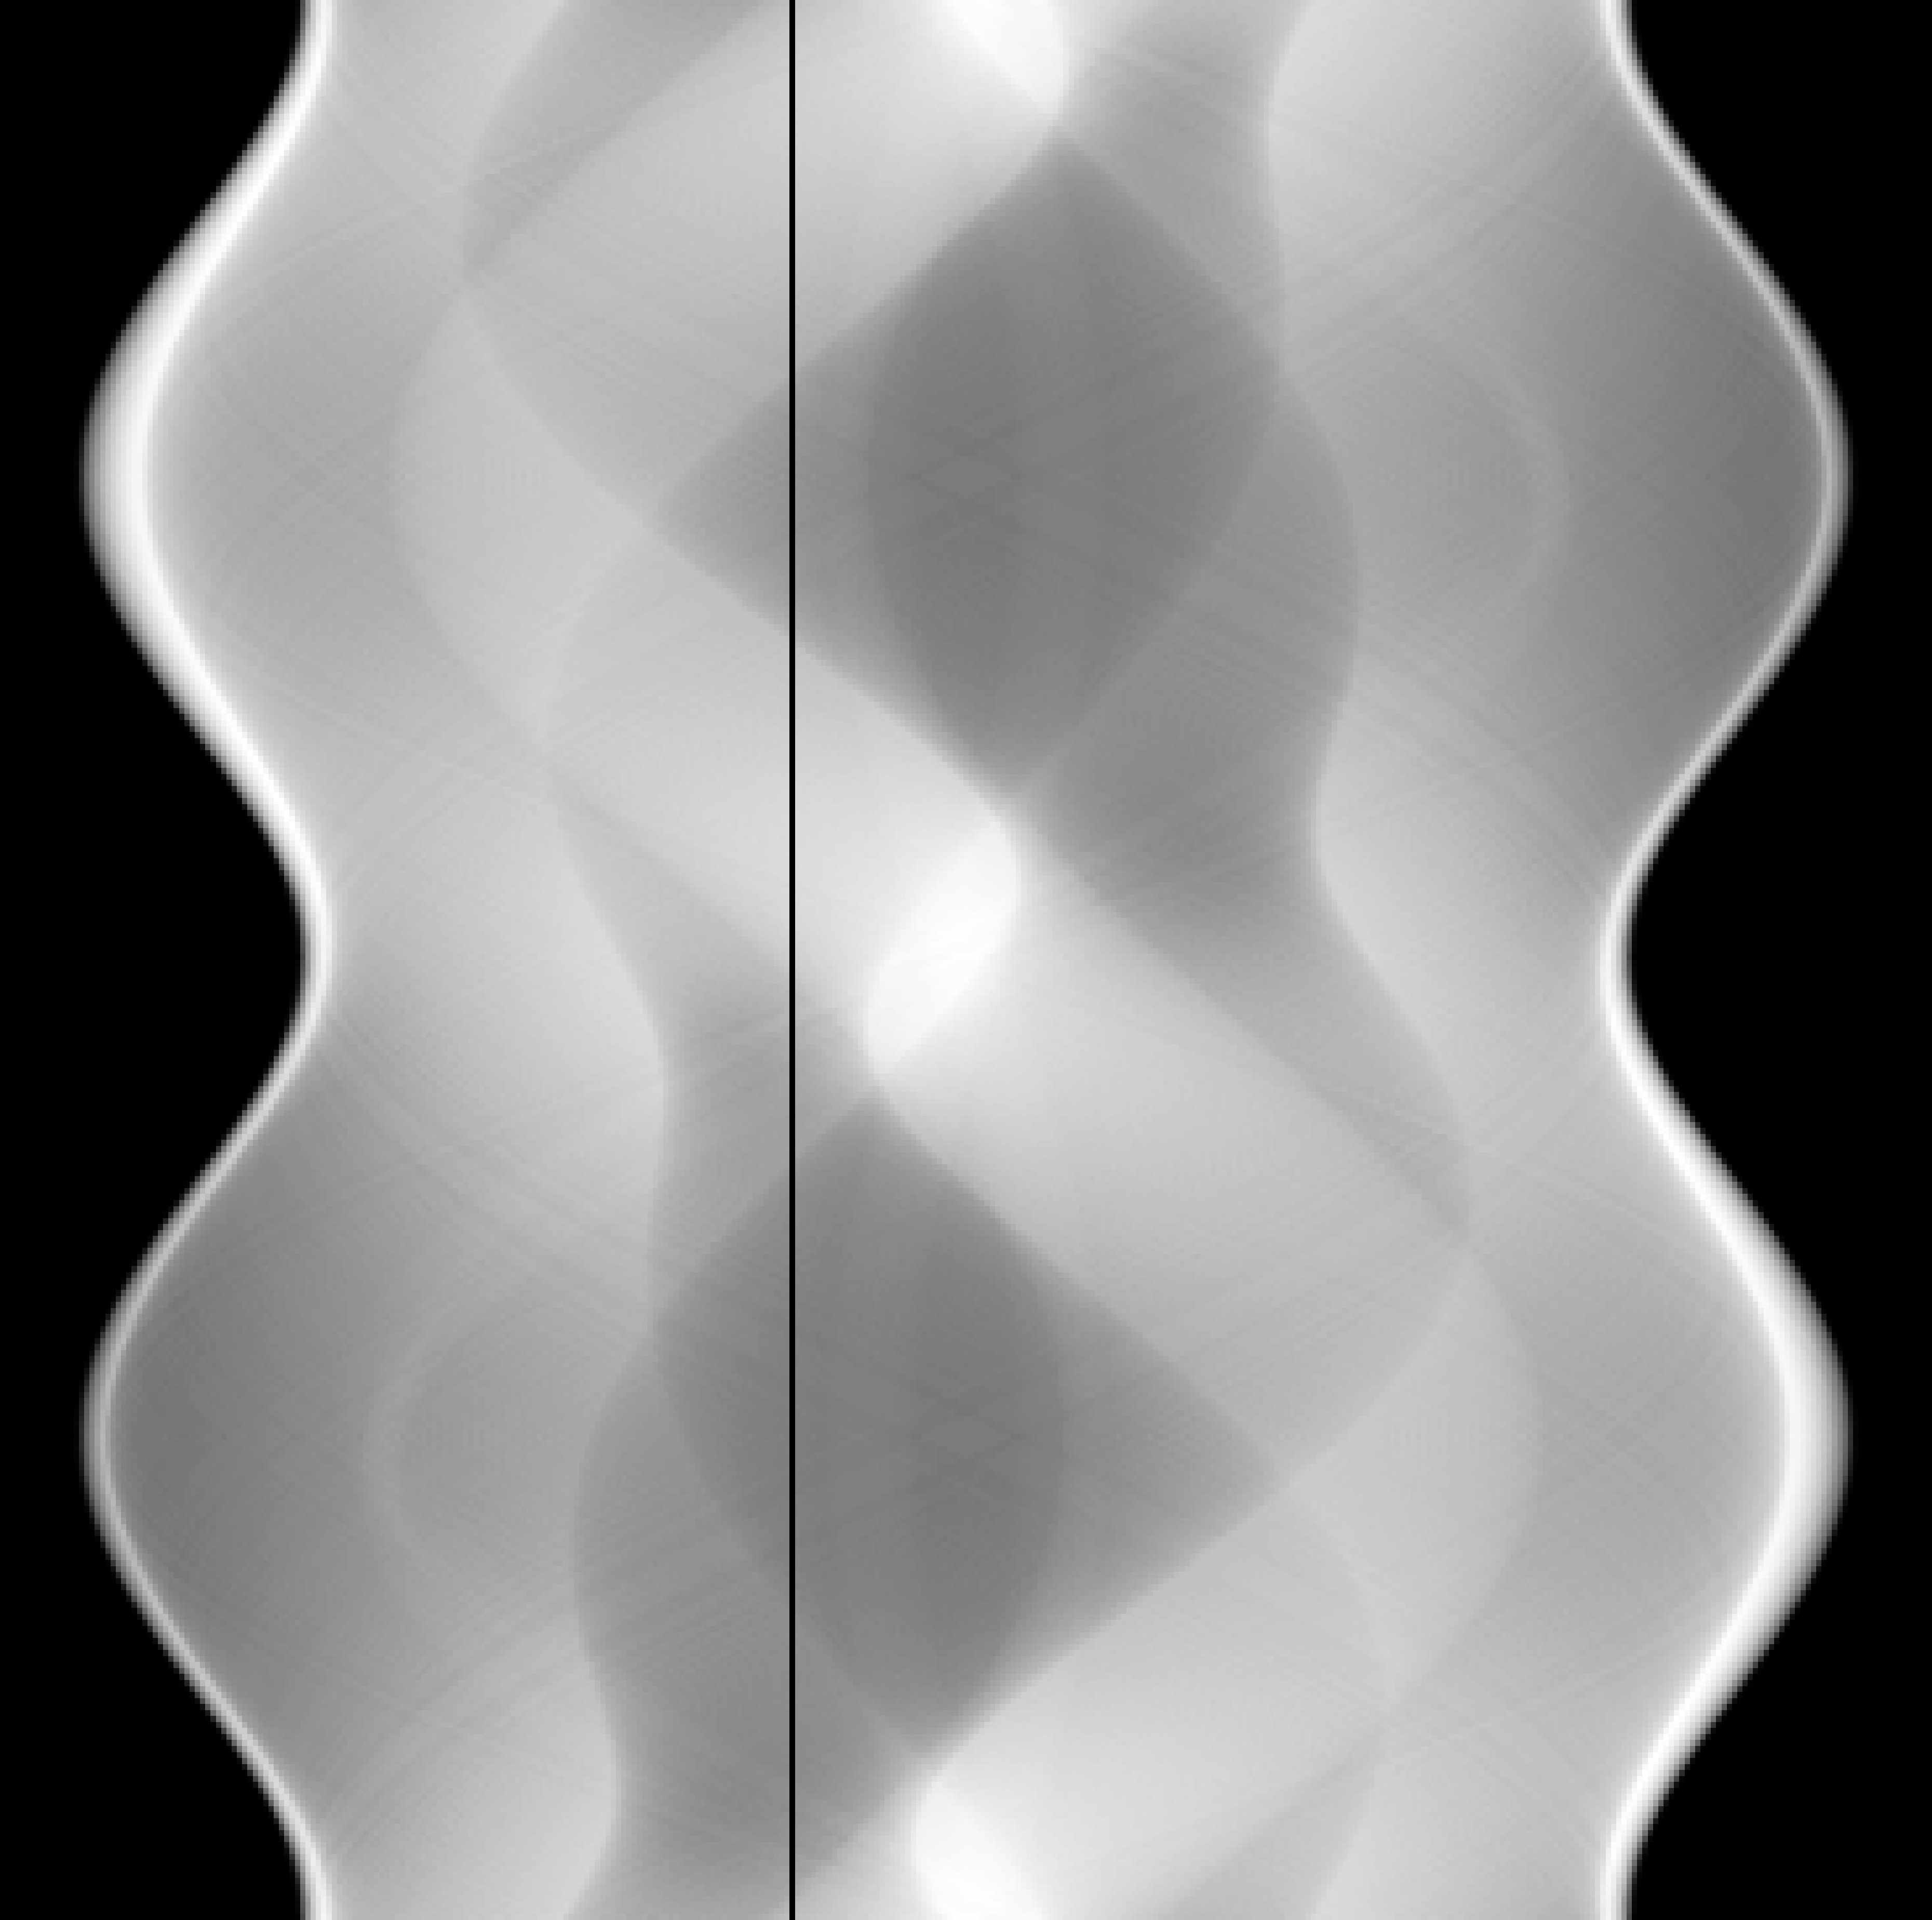
\includegraphics[width=\textwidth]{Figuras/sinograma_150.png}
       \end{subfigure}
       \begin{subfigure}[h]{0.24\textwidth}
           \centering
           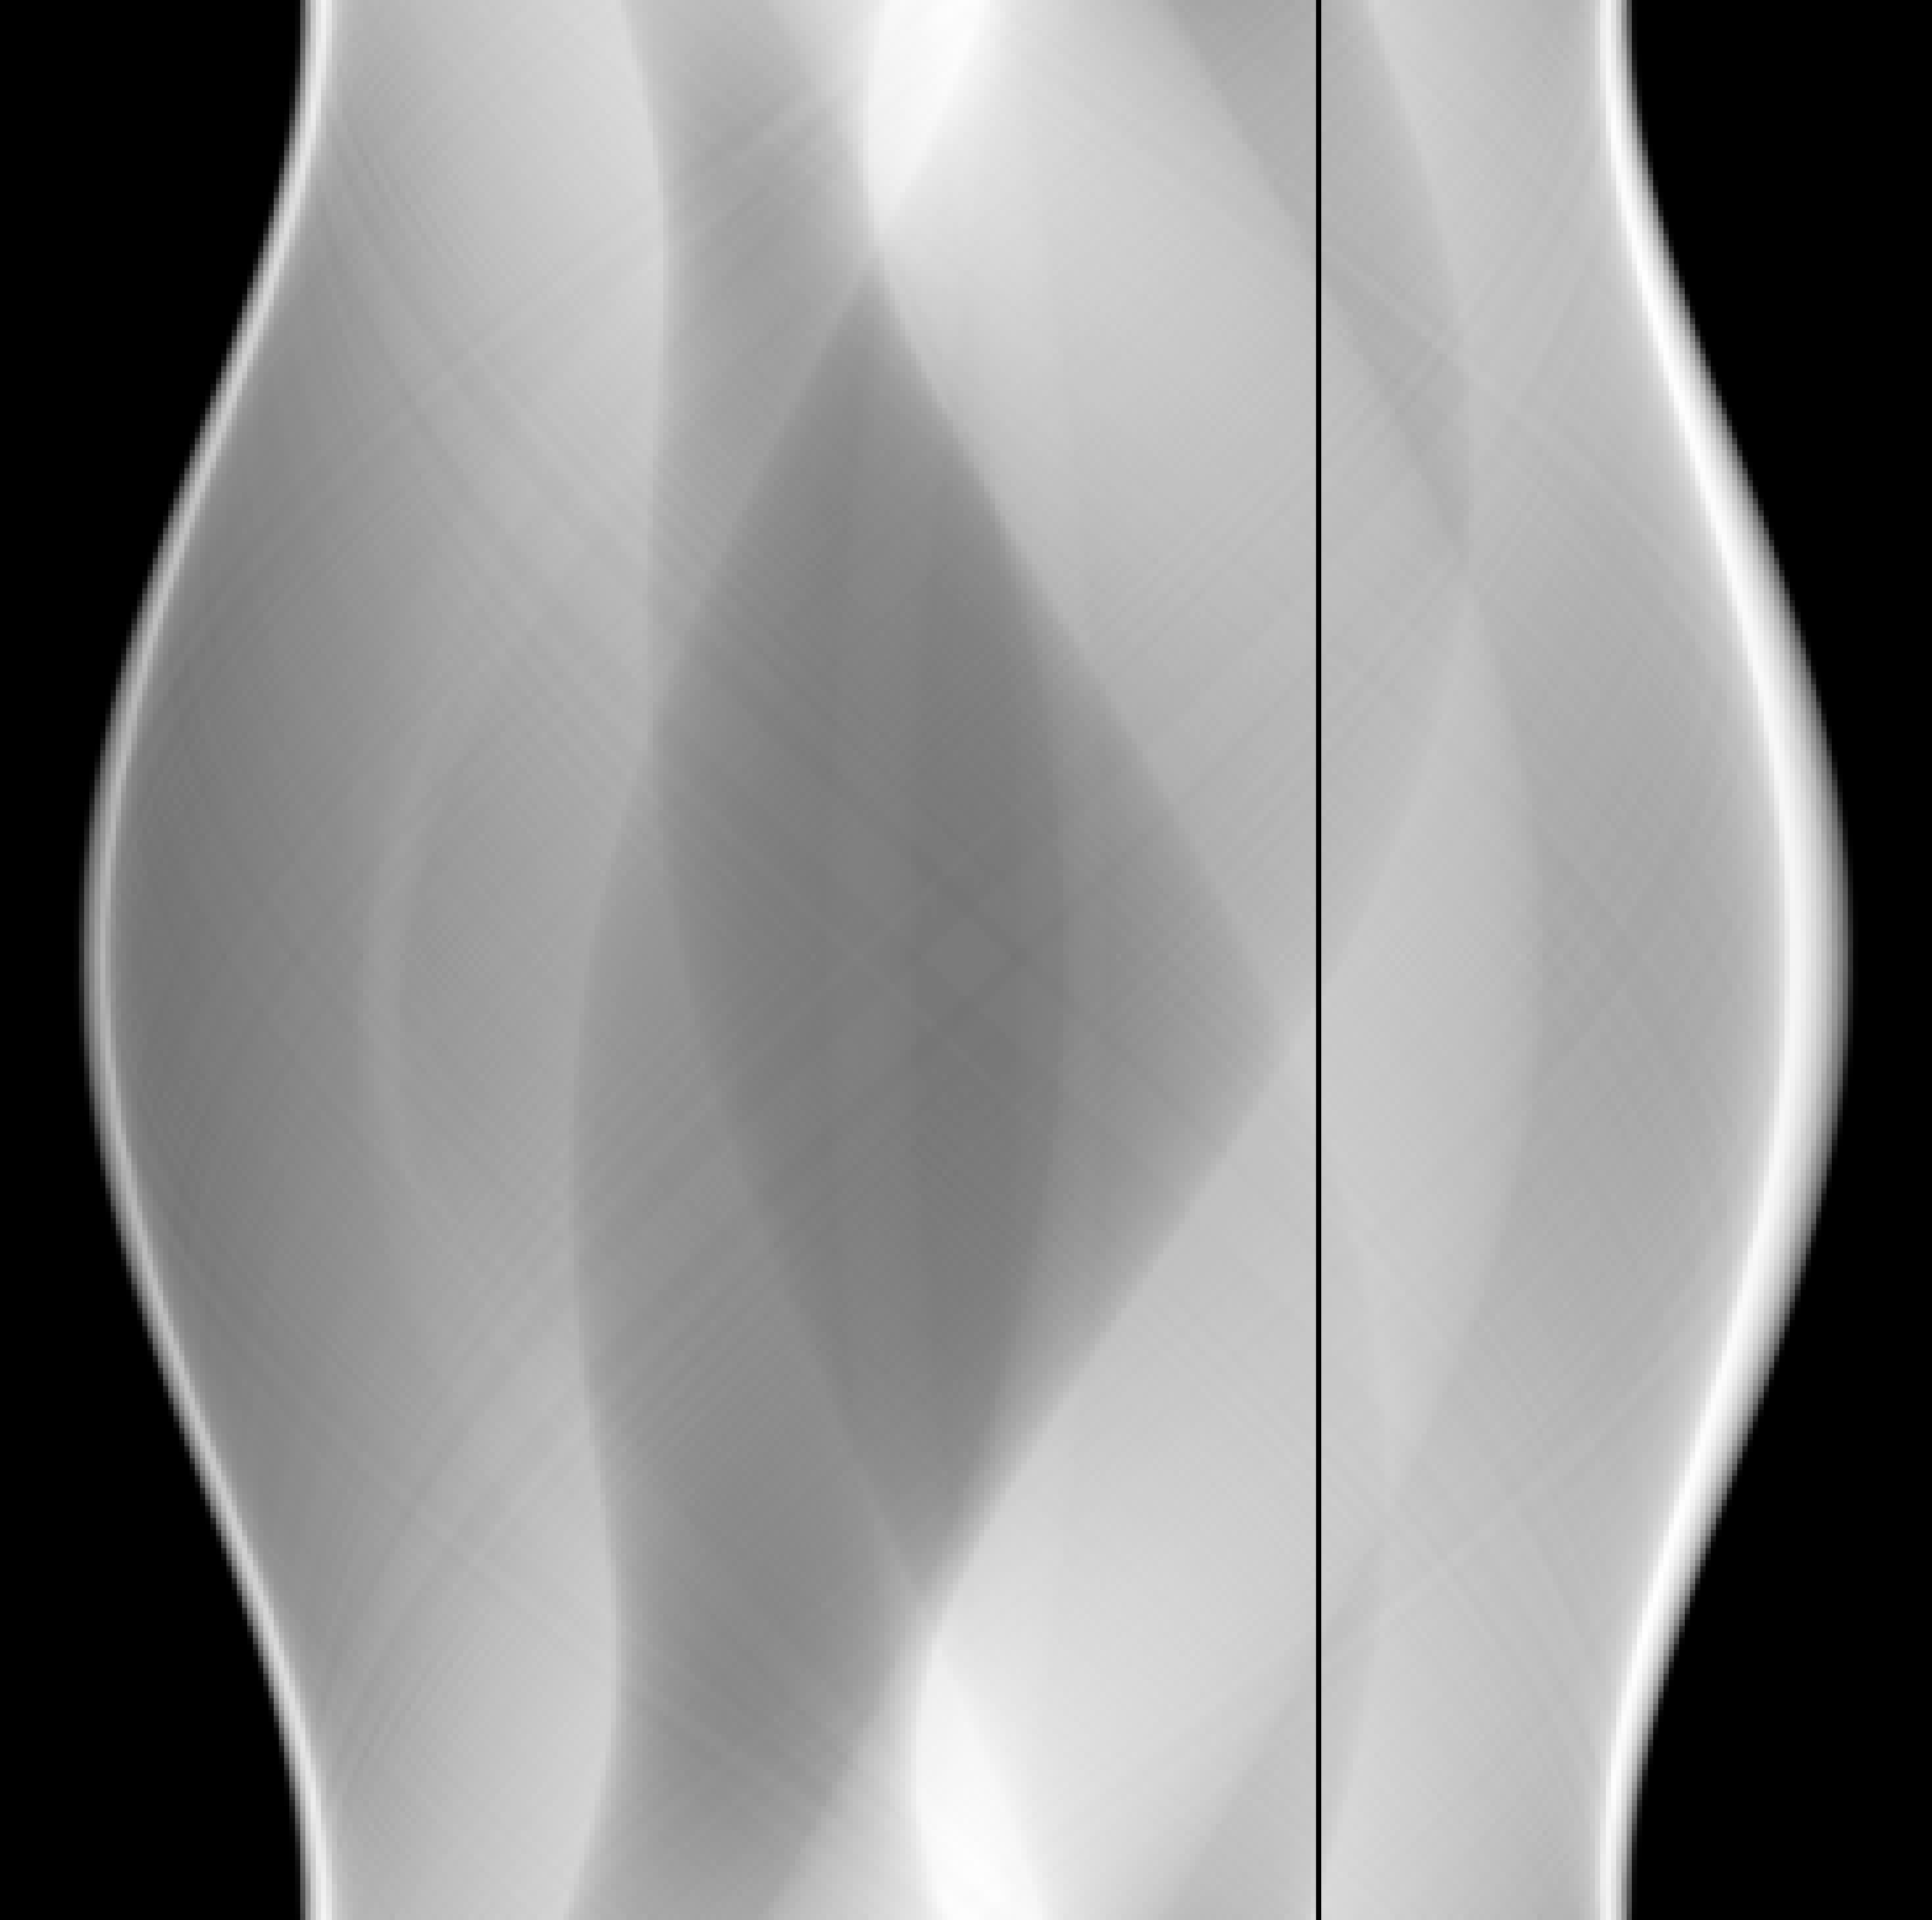
\includegraphics[width=\textwidth]{Figuras/sinograma_250.png}
       \end{subfigure}
       \begin{subfigure}[h]{0.24\textwidth}
           \centering
           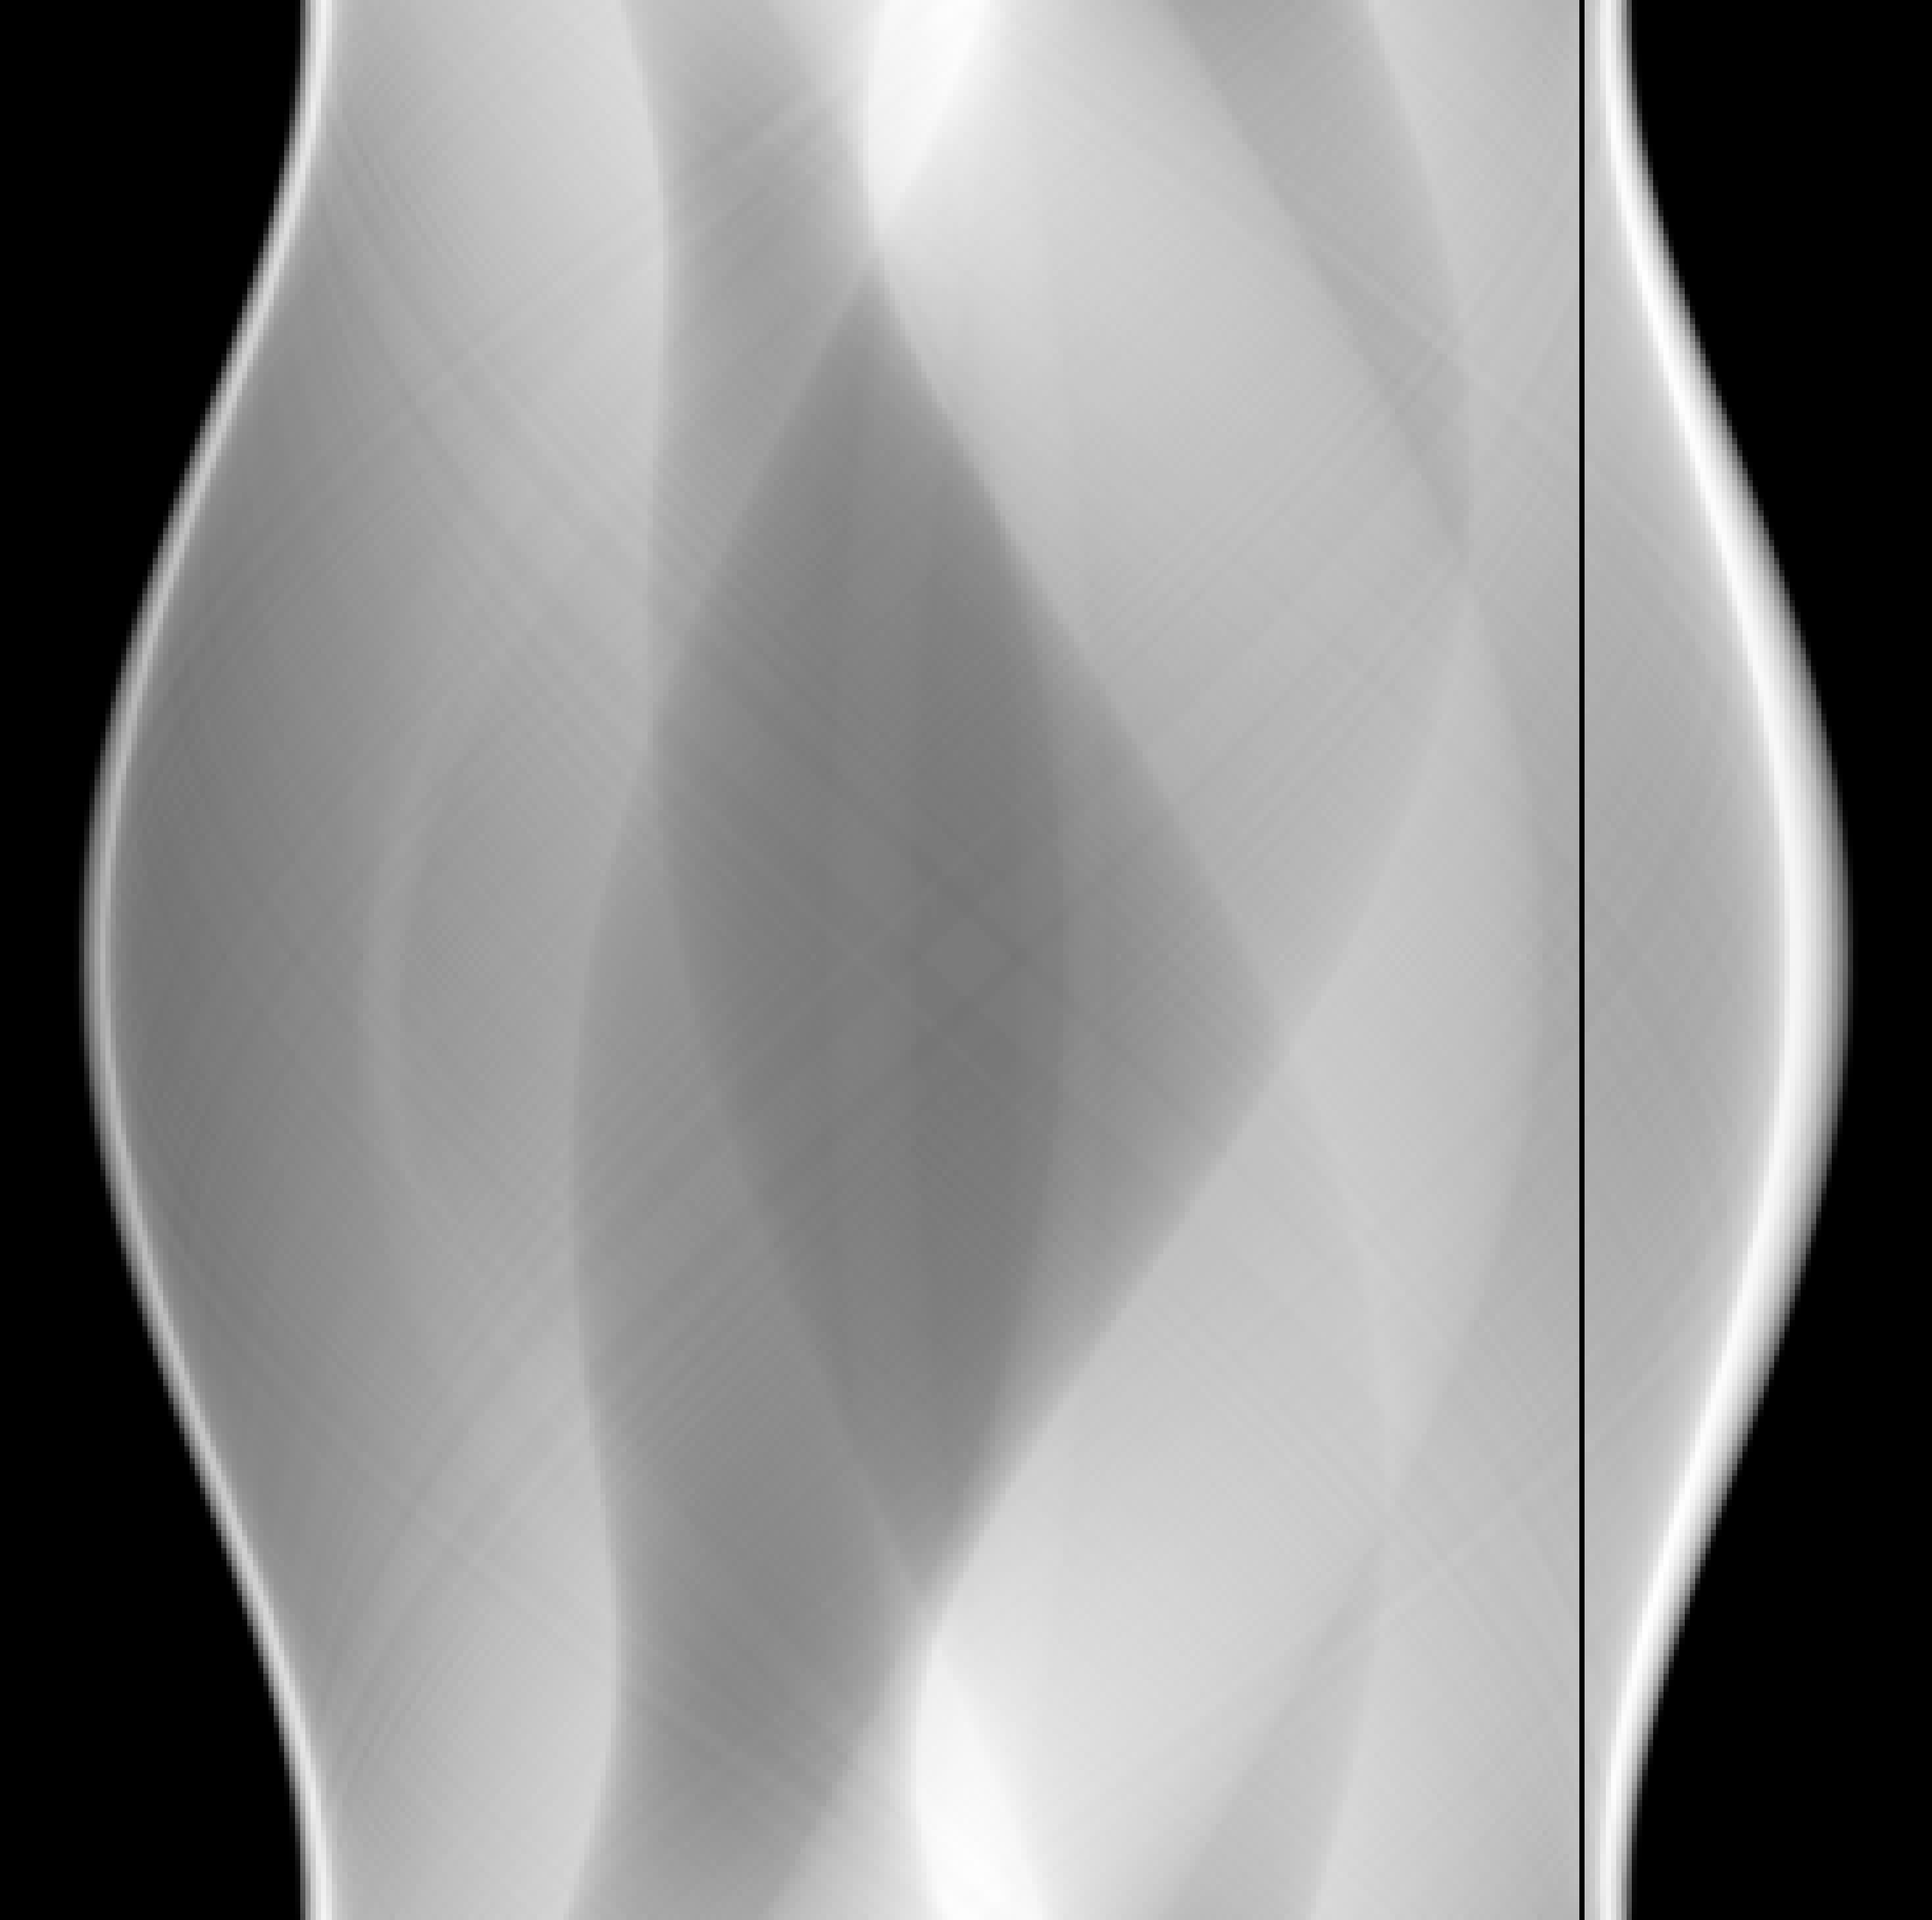
\includegraphics[width=\textwidth]{Figuras/sinograma_300.png}
       \end{subfigure}
        \begin{subfigure}[h]{0.24\textwidth}
           \centering
           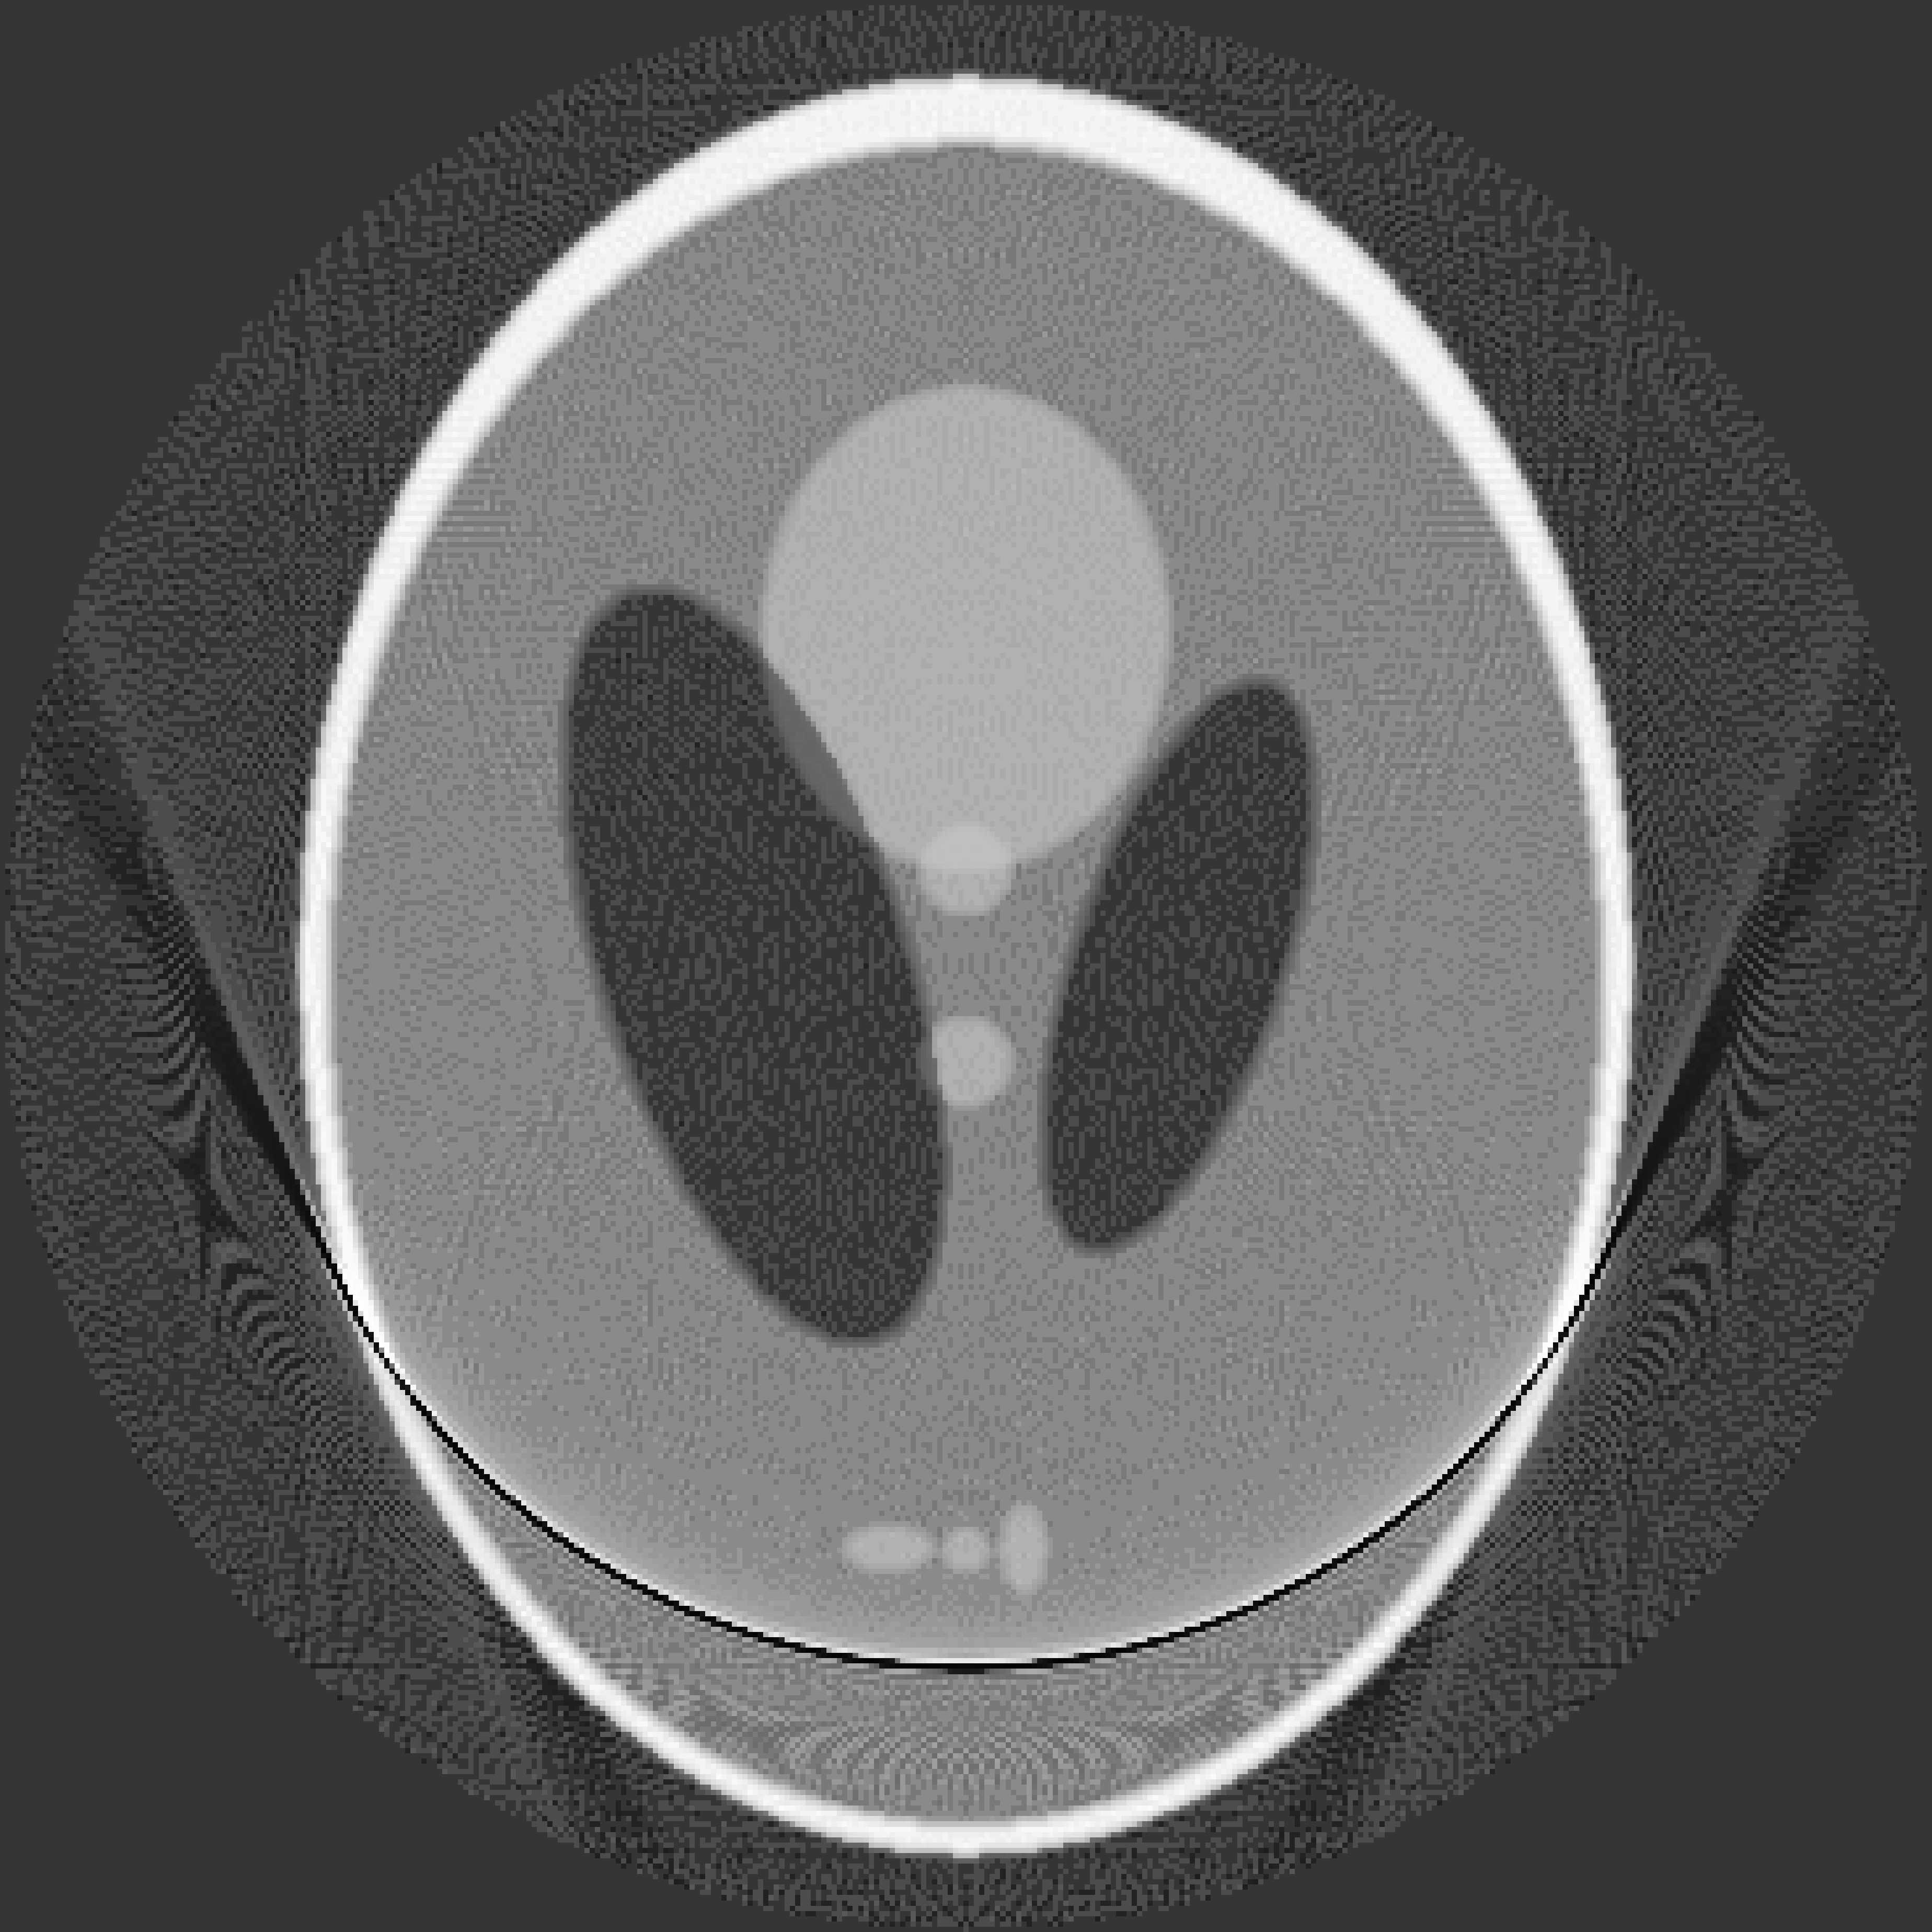
\includegraphics[width=\textwidth]{Figuras/reconstruction_50_EQ.png}
           \caption{Detector 50 defectuoso.} 
           \label{fig:sinograma_50}
        \end{subfigure}
        \begin{subfigure}[h]{0.24\textwidth}
           \centering
           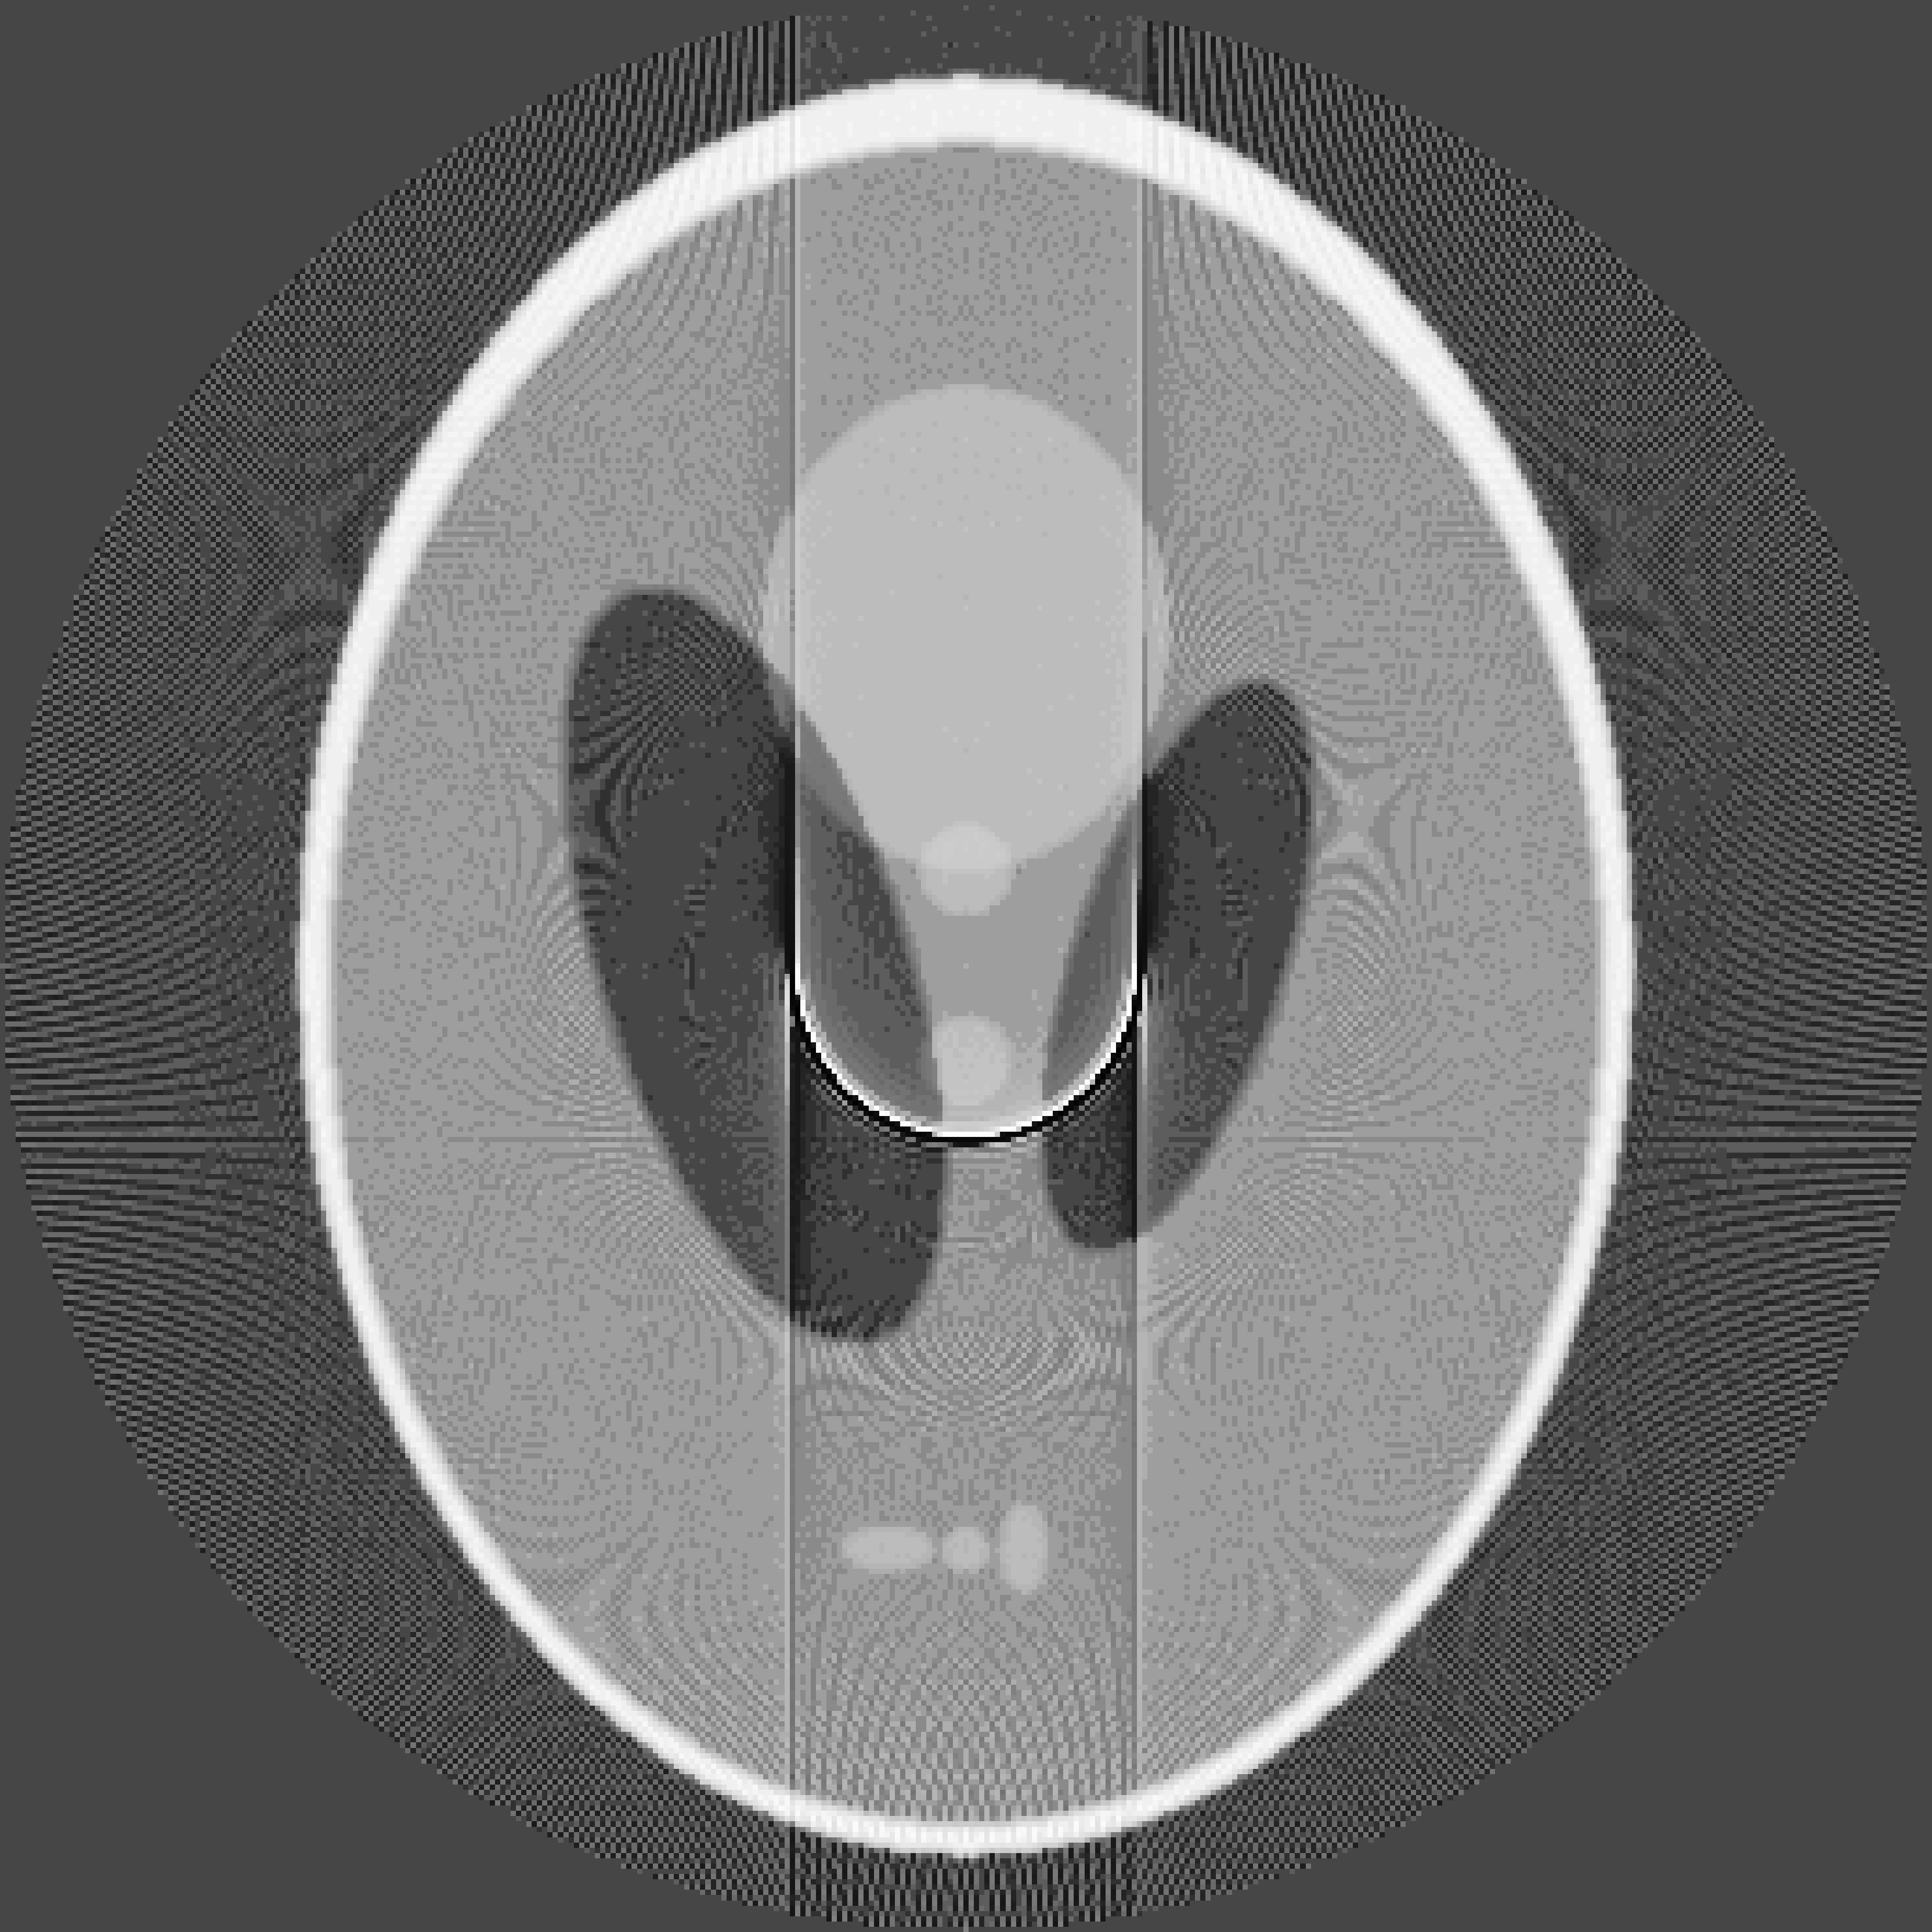
\includegraphics[width=\textwidth]{Figuras/reconstruction_150_EQ.png}
           \caption{Detector 150 defectuoso.} 
           \label{fig:sinograma_150}
        \end{subfigure}
        \begin{subfigure}[h]{0.24\textwidth}
           \centering
           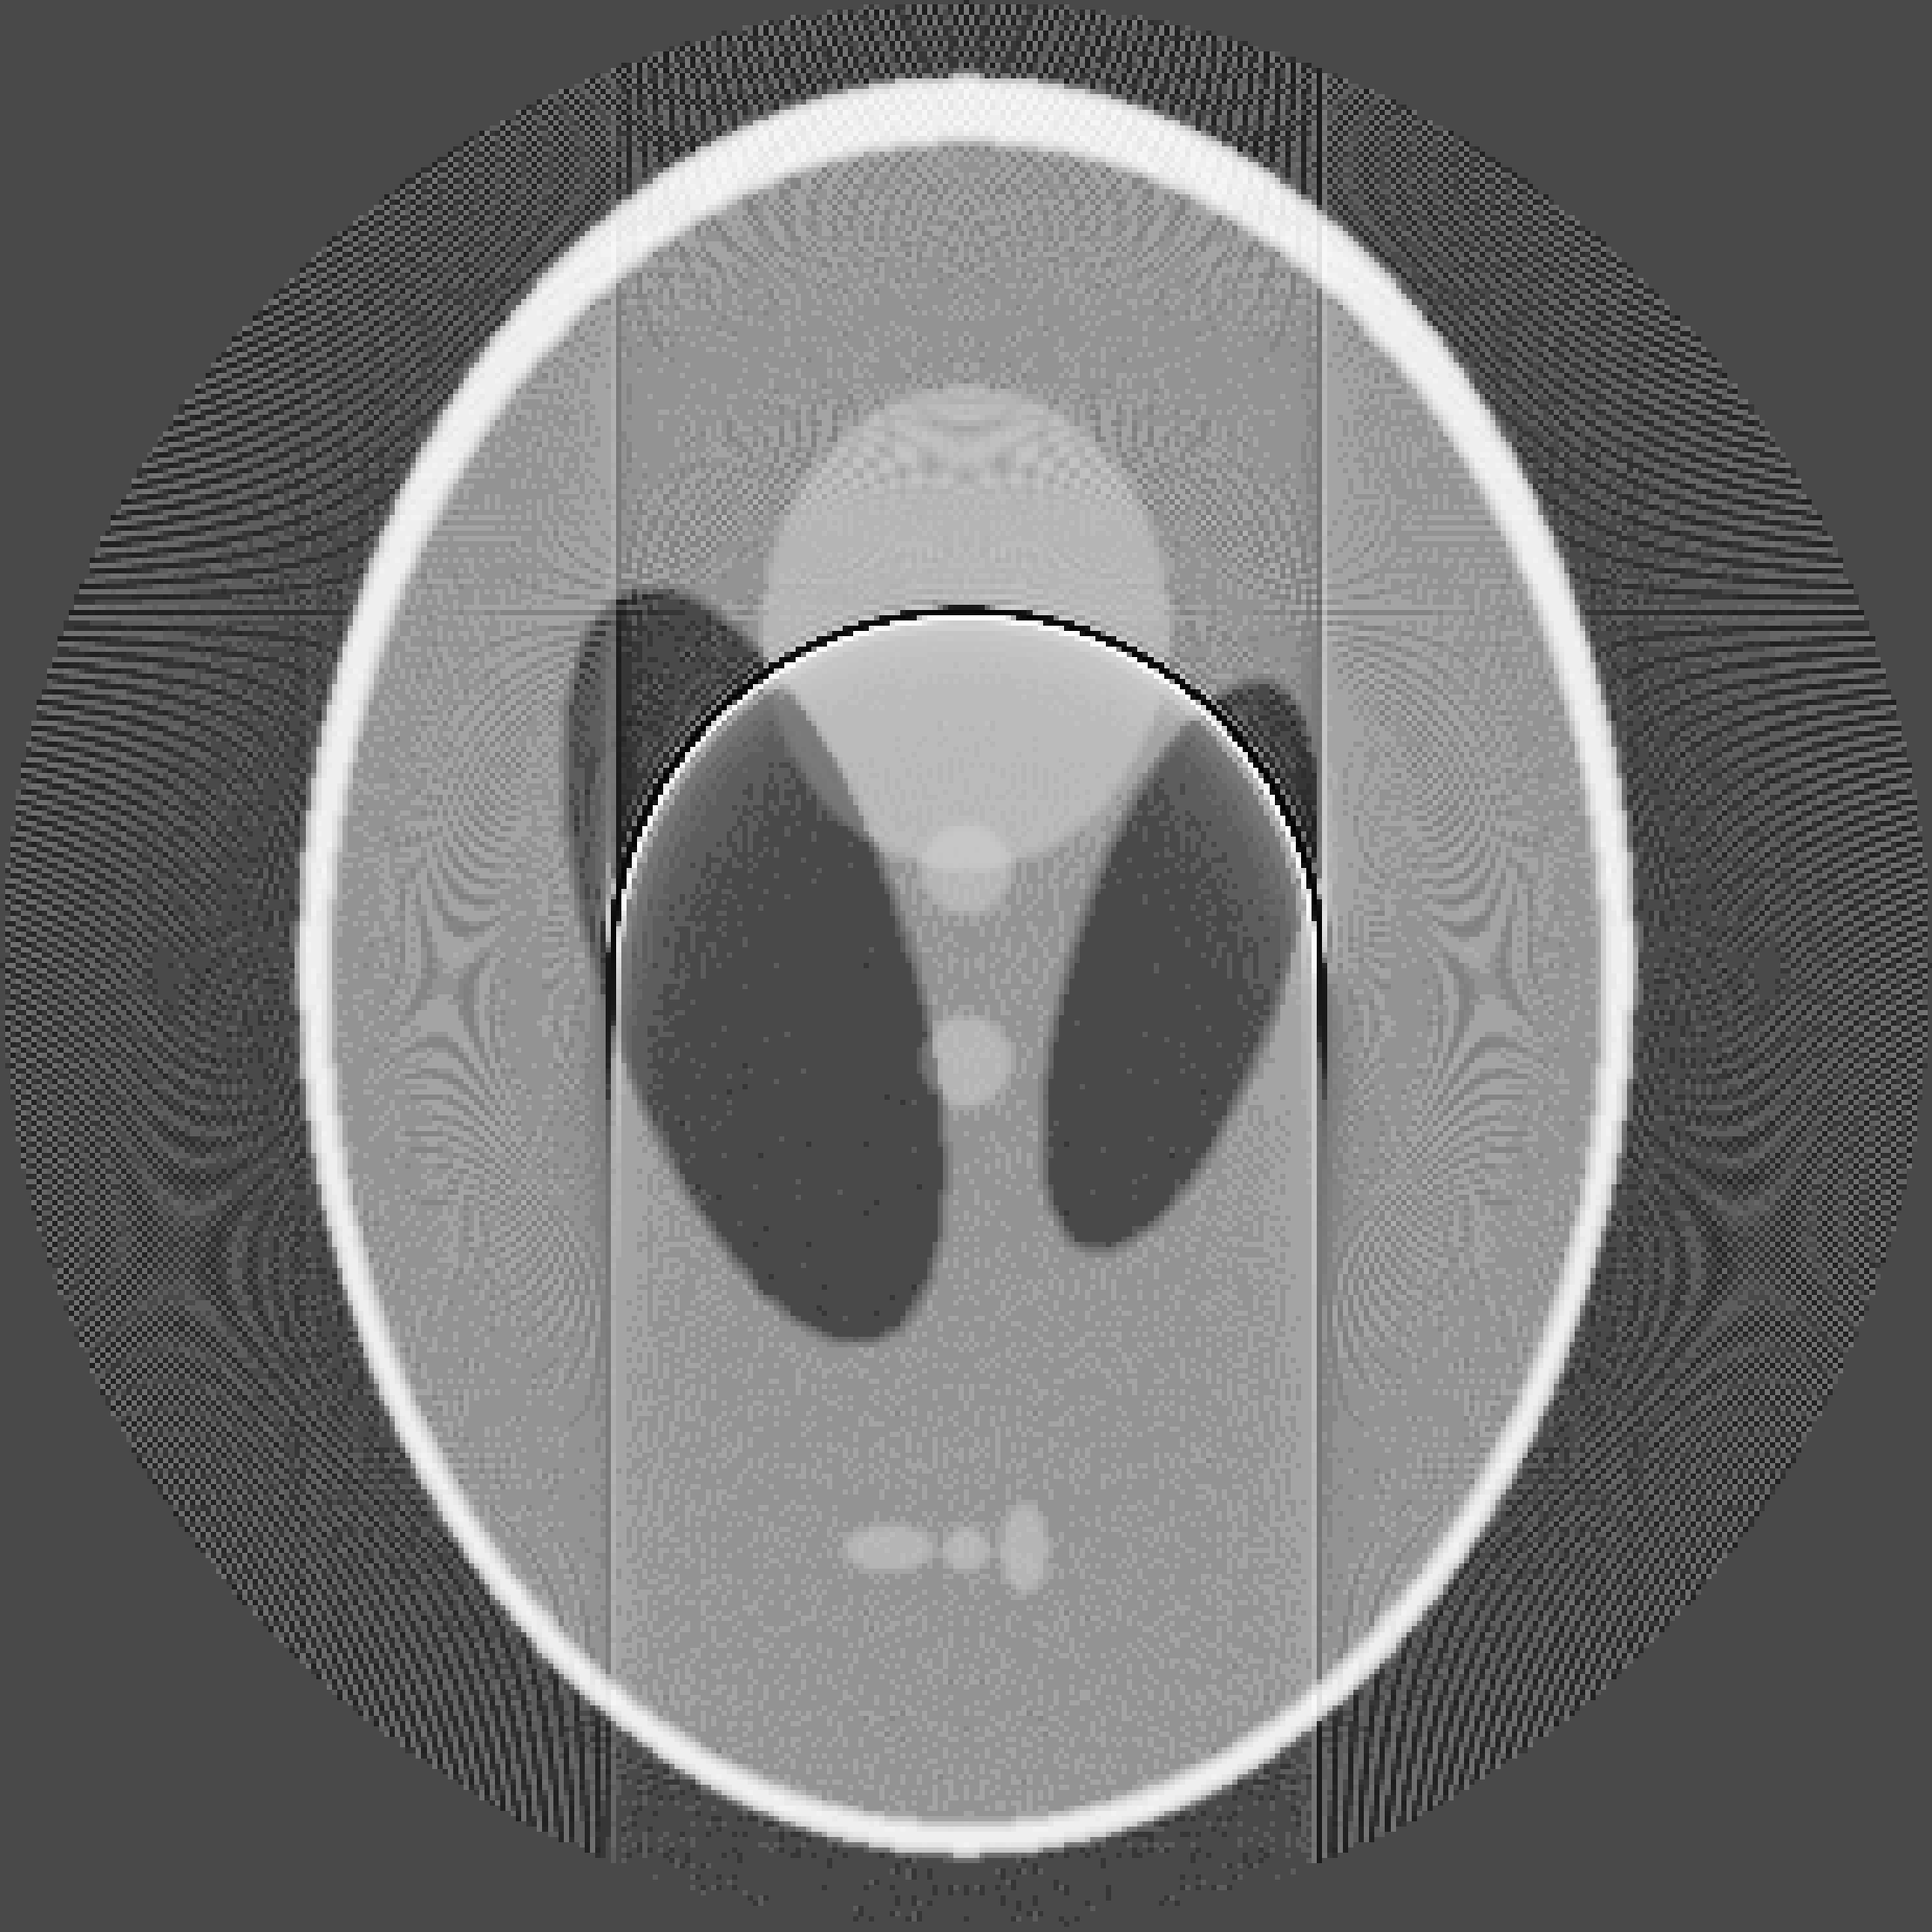
\includegraphics[width=\textwidth]{Figuras/reconstruction_250_EQ.png}
           \caption{Detector 250 defectuoso.}
           \label{fig:sinograma_250} 
        \end{subfigure}
        \begin{subfigure}[h]{0.24\textwidth}
           \centering
           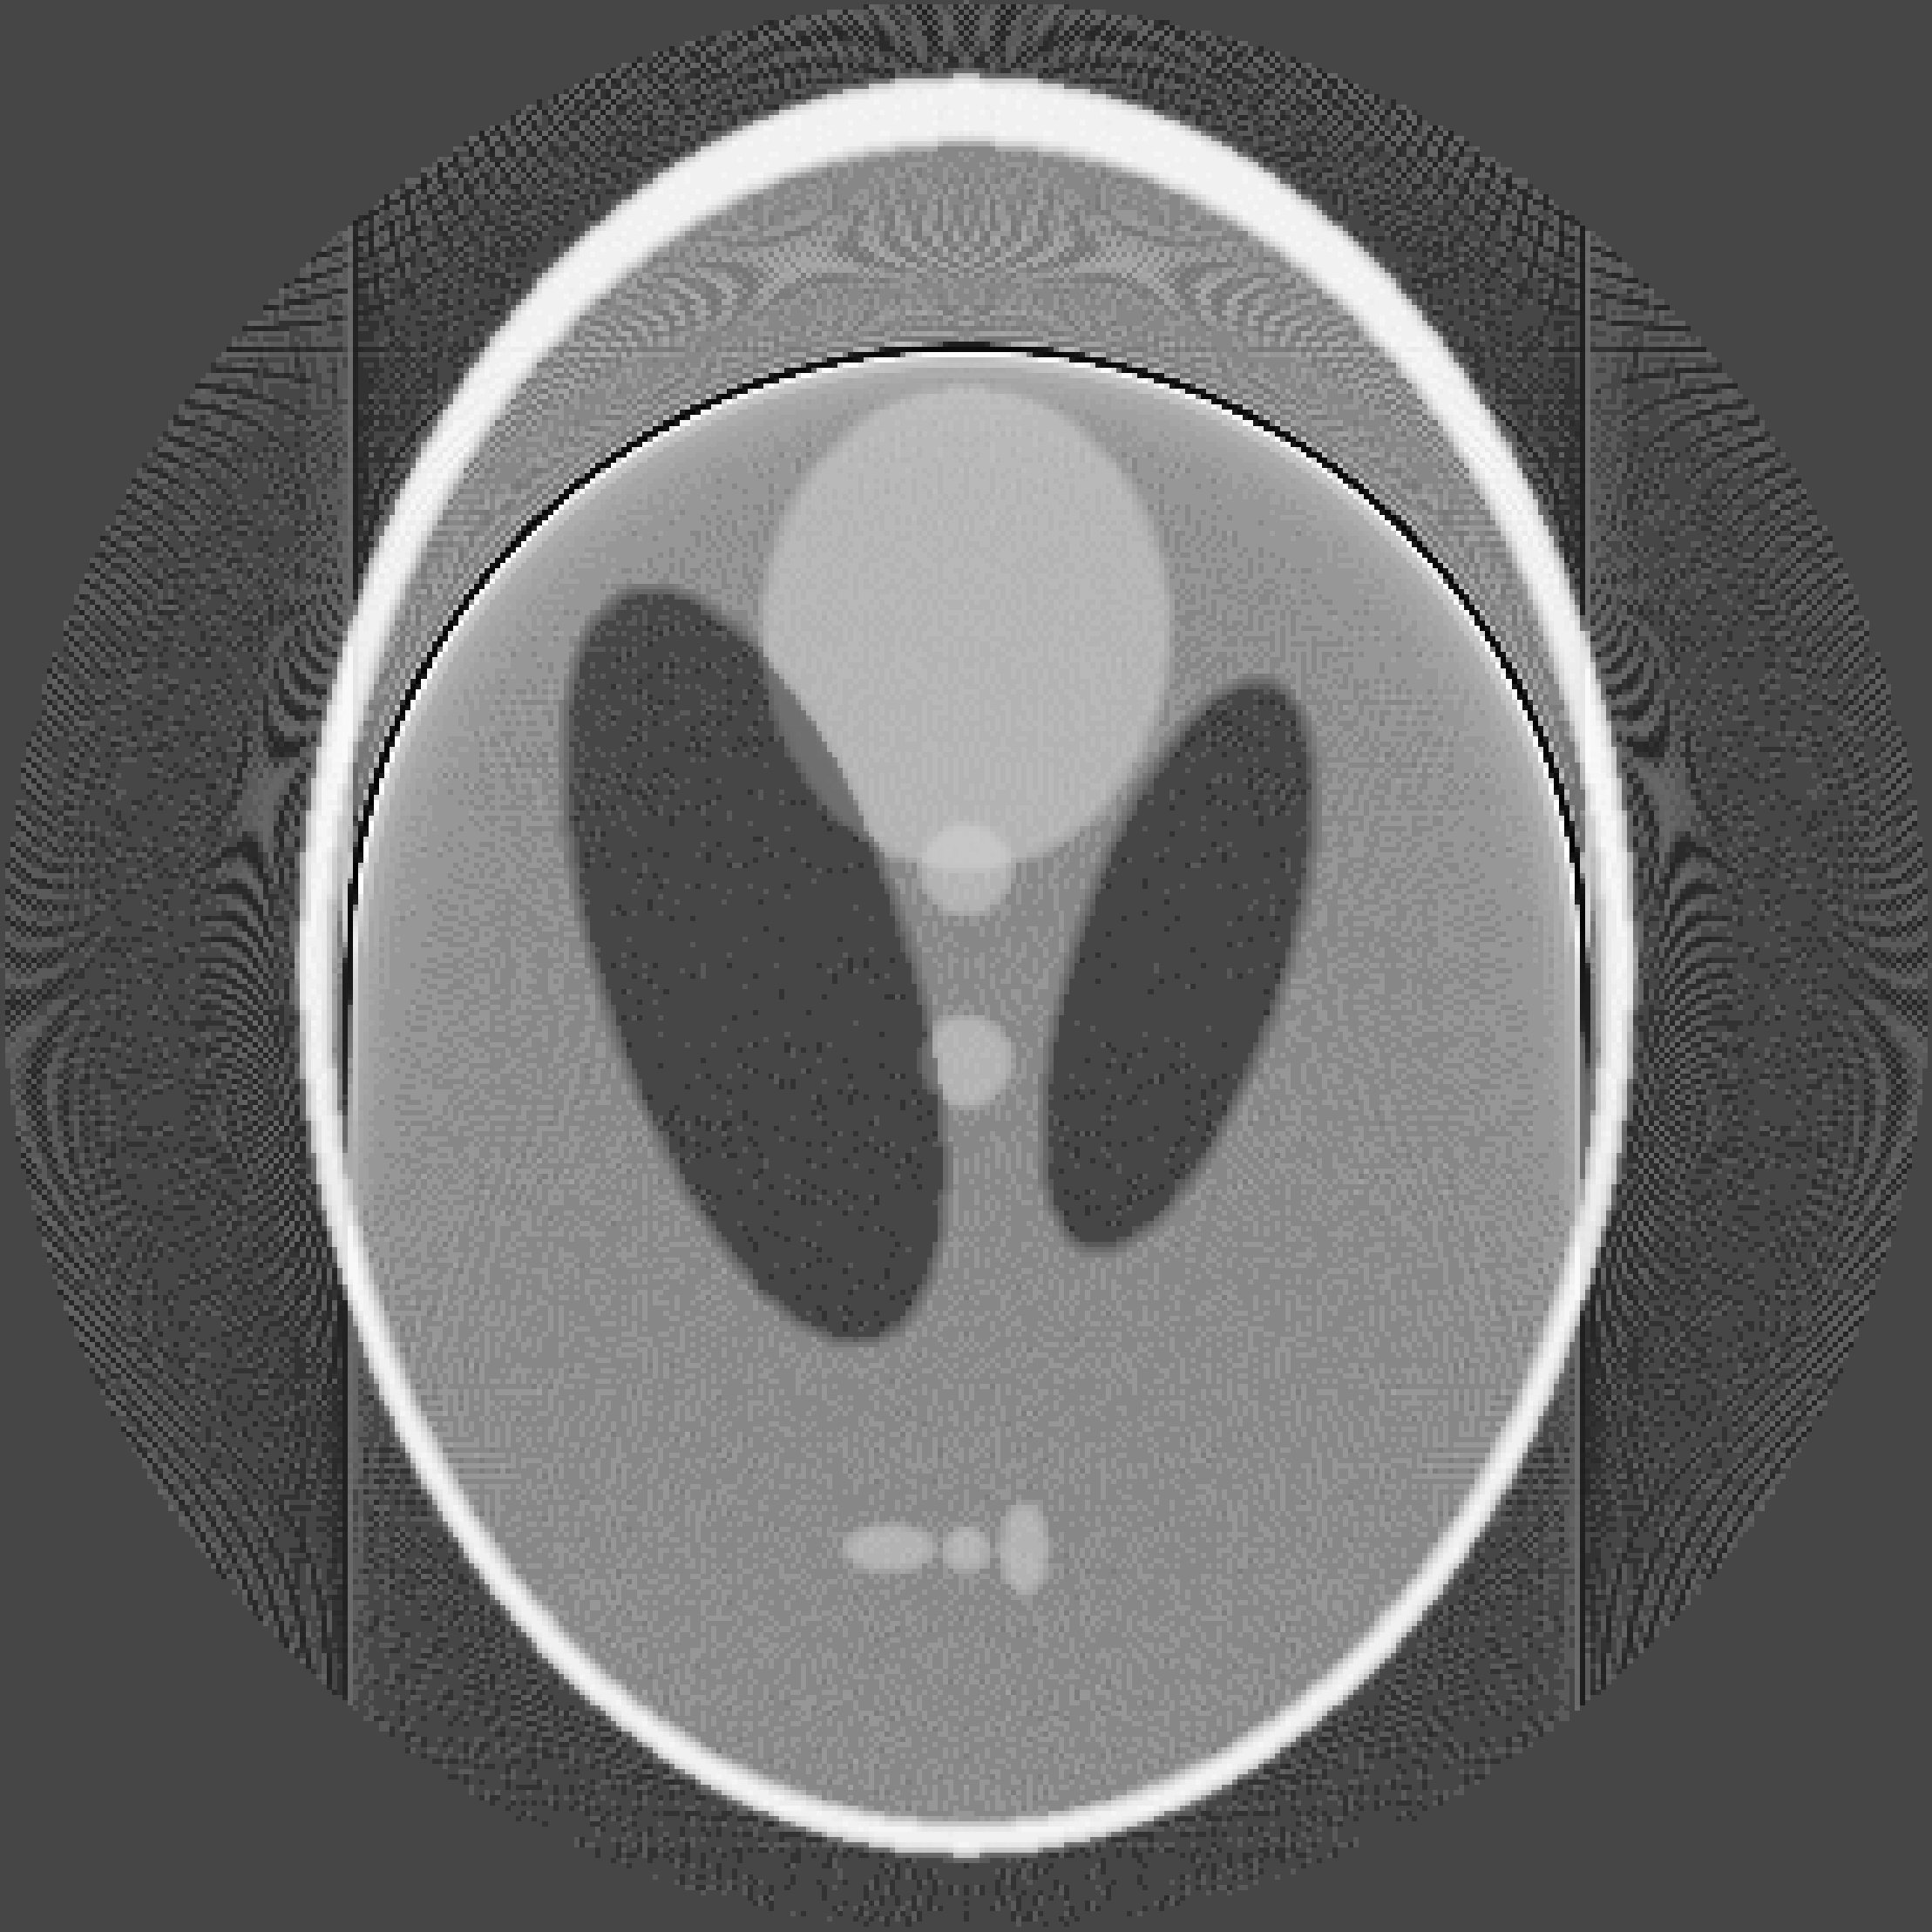
\includegraphics[width=\textwidth]{Figuras/reconstruction_300_EQ.png}
           \caption{Detector 300 defectuoso.}
           \label{fig:sinograma_300} 
        \end{subfigure}
   \caption{Sinogramas generados con 367 detectores y 320 proyecciones. Arriba: Sinogramas con defectos en los detectores 50, 150, 250 y 300 que no registran actividad. Abajo: Retroproyección con filtro rampa de los sinogramas con defectos, estas imagenes fueron ecualizadas.}
   \label{fig:detector_roto}
\end{figure}

Por último, si el sinograma se genera recorriendo la circunferencia completa, el resultado defecto es un circulo completo con cuatro lineas tangentes al circulo. En la Fig. \ref{fig:comp_defecto} se muestra la comparación entre las retroproyecciones filtradas a partir de un sinograma que no registra actividad en el detector 150 obtenido recorriendo una circunferencia completa y media circunferencia.


\begin{figure}[H]
   \centering
        \begin{subfigure}[h]{0.49\linewidth}
           \centering
           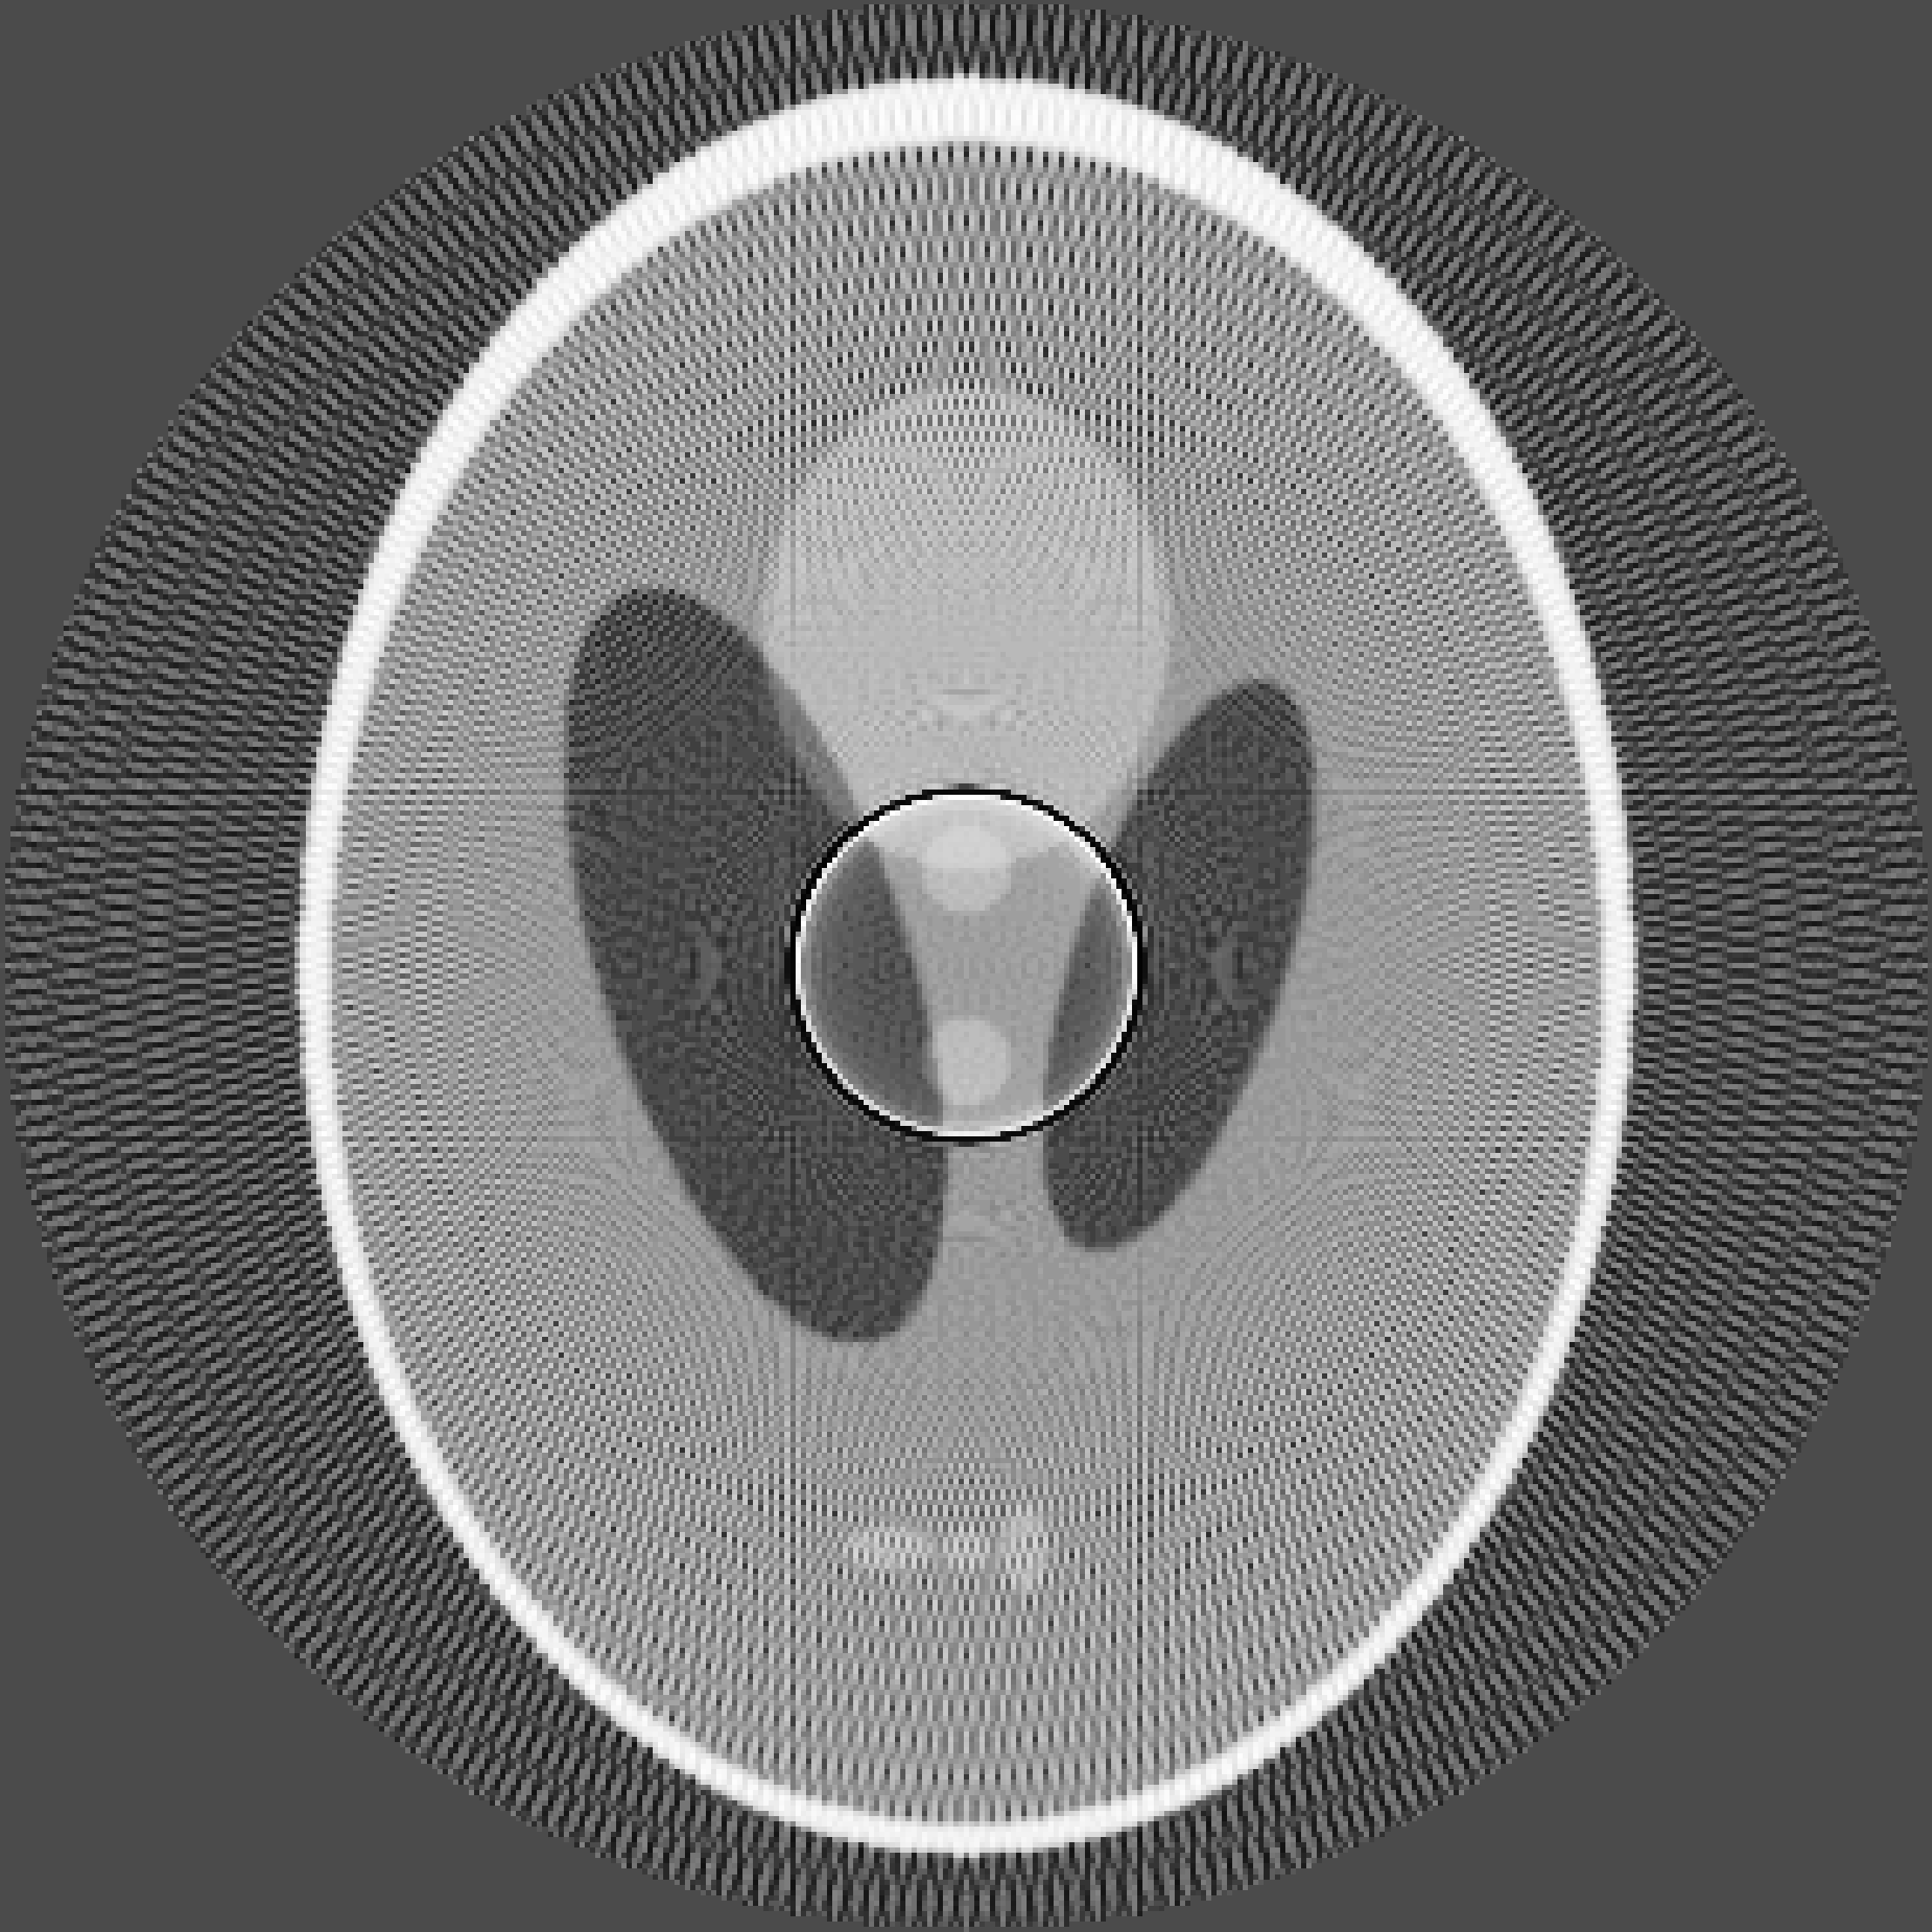
\includegraphics[width=0.8\textwidth]{Figuras/reconstruction_150_360_EQ.png}
           \caption{Sinograma de circunferencia completa.} 
           \label{fig:defecto_360}
        \end{subfigure}
        \begin{subfigure}[h]{0.49\linewidth}
           \centering
           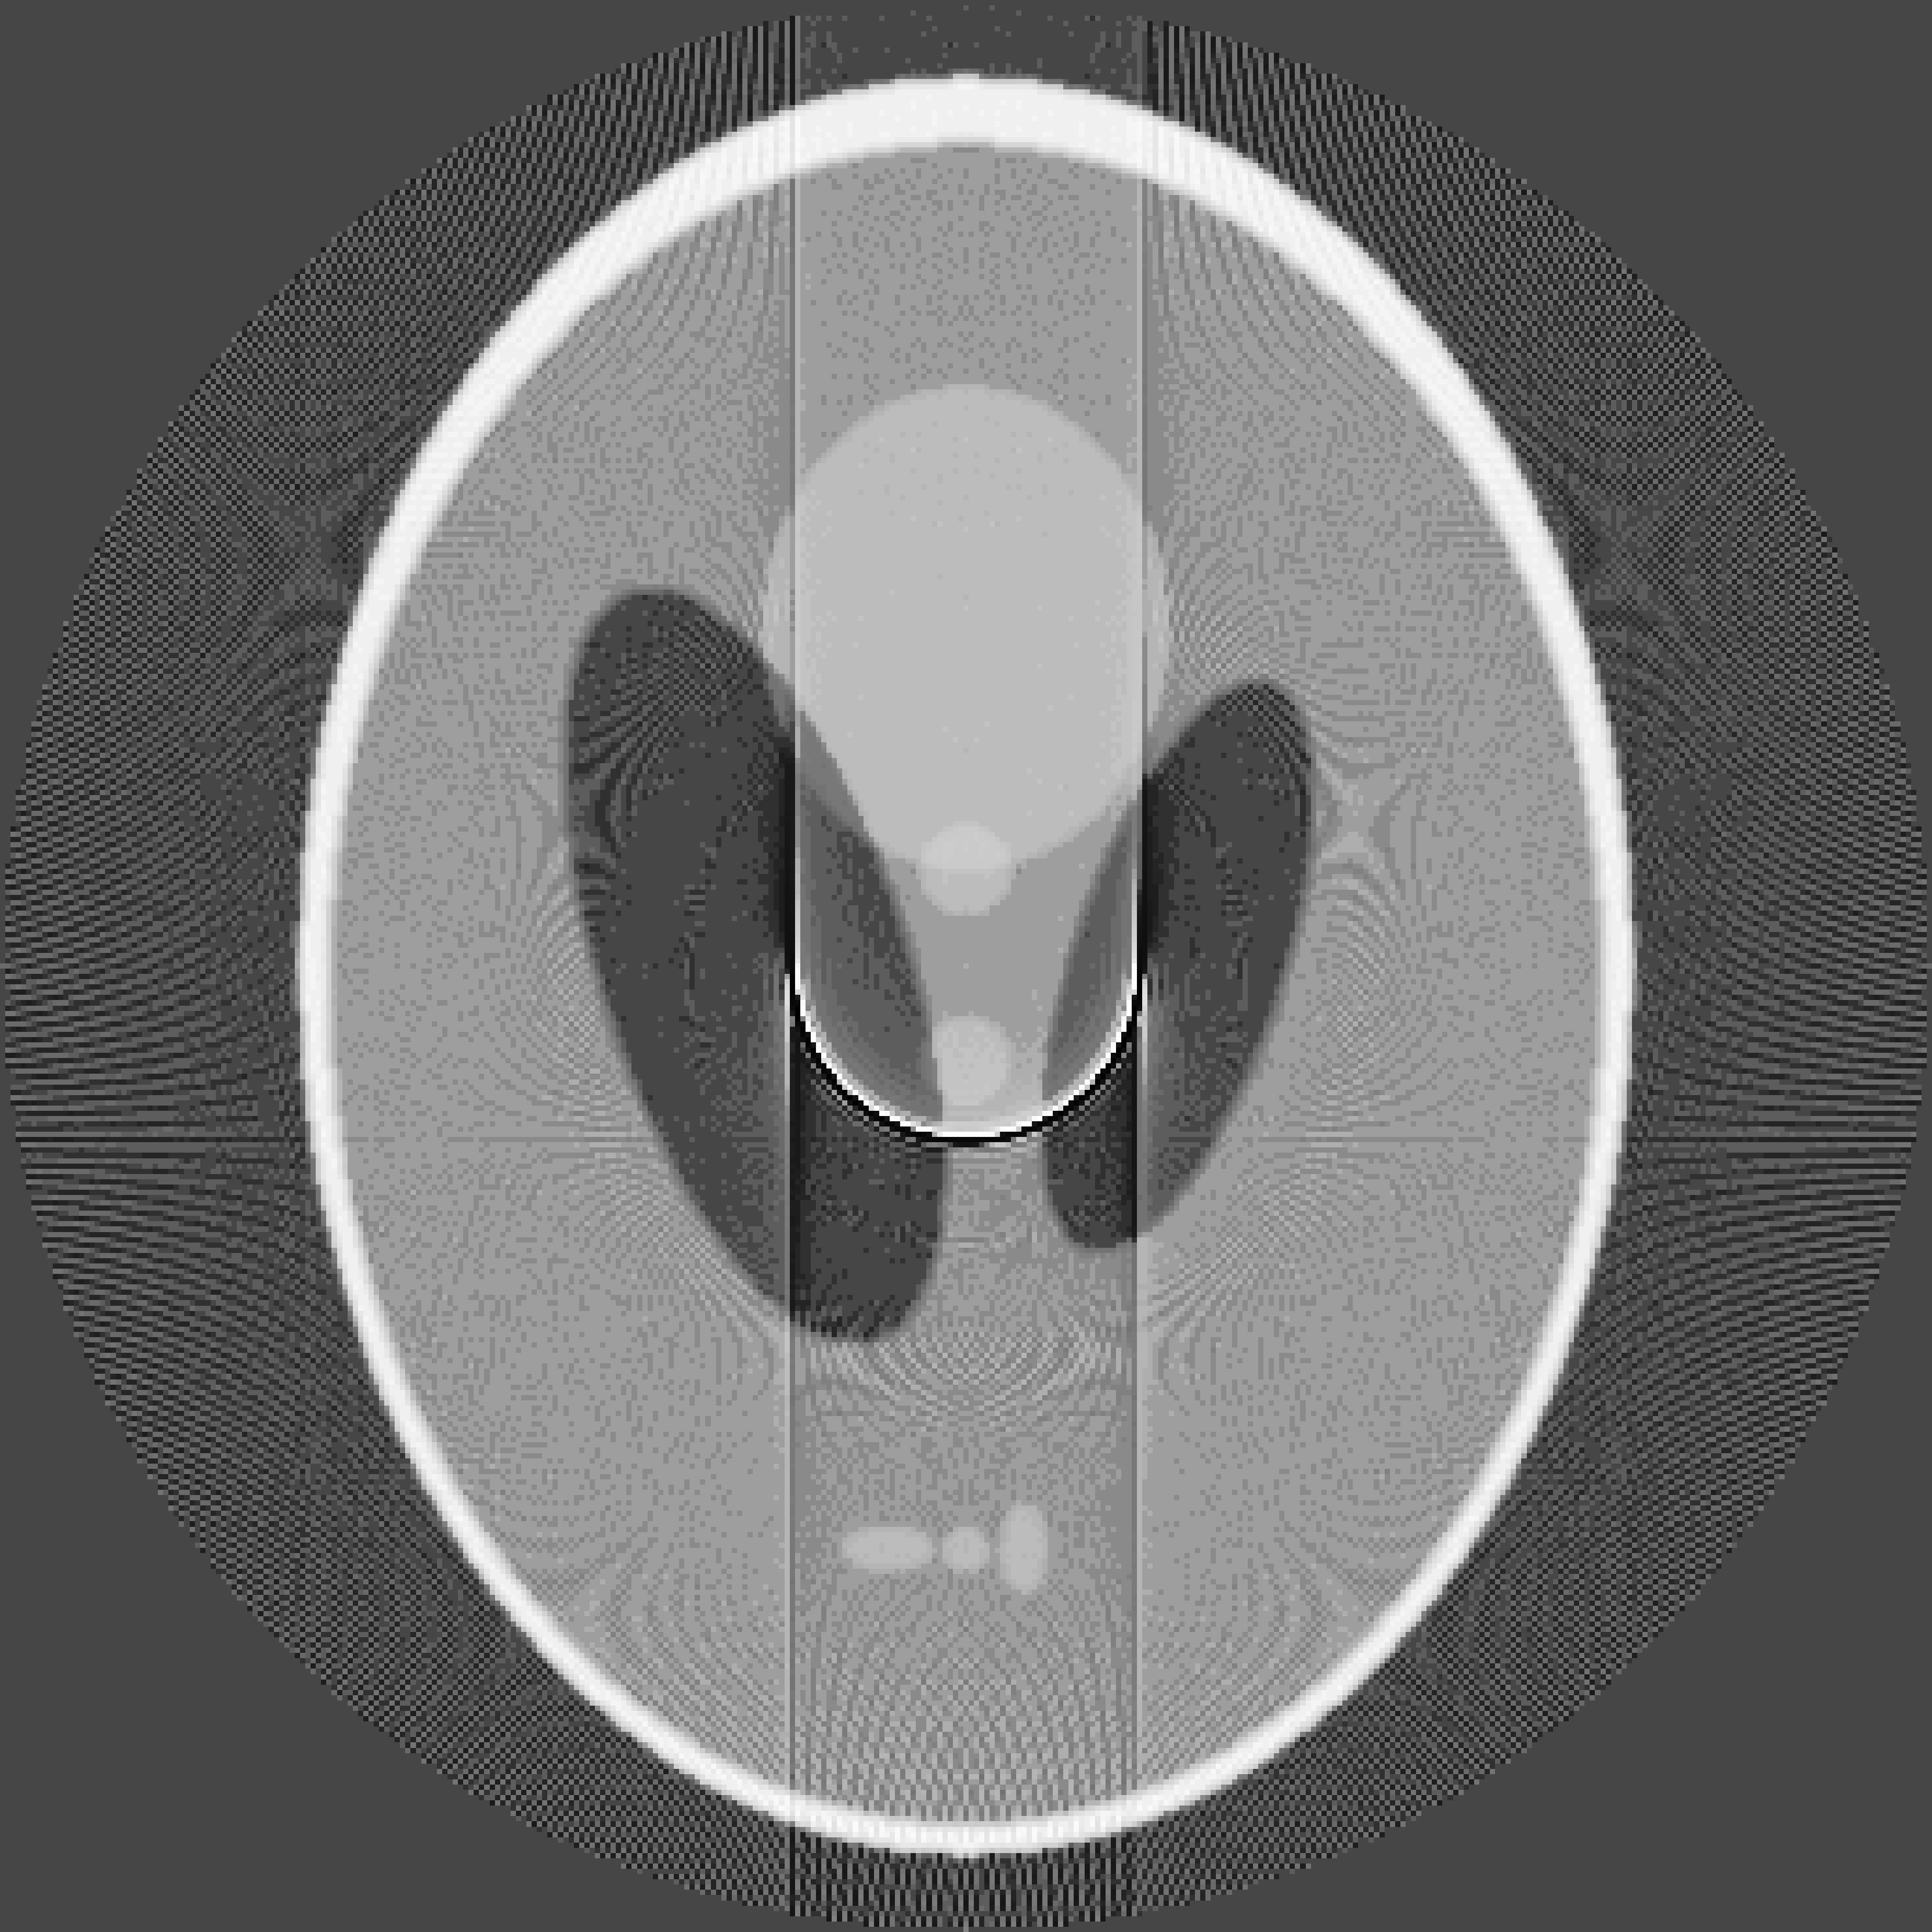
\includegraphics[width=0.8\textwidth]{Figuras/reconstruction_150_EQ.png}
           \caption{Sinograma de media circunferencia.}
           \label{fig:defecto_180}
        \end{subfigure}
   \caption{Comparación entre las retroproyecciones filtradas a partir de un sinograma obtenido recorriendo una circunferencia completa (a) y media circunferencia (b).}
   \label{fig:comp_defecto}
\end{figure}










\centerline{\rule{0.95\linewidth}{0.6pt}}


%\bibliographystyle{plain} % Estilo de bibliografía
%\bibliography{bibliography}    % Nombre de tu archivo .bib sin la extensión


\end{document}